% =============================================================================
%  SOUTENANCE INSTITUT DES ACTUAIRES, version complète du support (environ 70
%  diapositives, annexes comprises), qui suit le mémoire Institut chapitre par chapitre.
%  La version ENSAE de 15 minutes (soutenance_ensae.tex) en est le résumé méthodologique,
%  adossé au rapport ENSAE : les deux fichiers ne lisent pas le même rapport (la descente
%  à l'échelle d'une entité diffère : partage de l'exposition dans l'Institut).
%  Support Beamer. Forme reprise de la présentation de
%  Lucas Offroy (navigation par section, une idée par diapositive, figures
%  légendées) ; contenu et consignes d'Hugo Rapior du 22 octobre 2026.
%
%  Les nombres viennent du rapport Institut (memoire/main_institut_150.pdf) ou des
%  compléments après dépôt explicitement cités (script 129, script 130).
%  Contrôle numérique, depuis la racine du dépôt :
%     .venv\Scripts\python.exe recherche\slides\beamer\controle_nombres.py
%       --deck recherche\slides\beamer\soutenance_institut.pdf --rapport memoire\main_institut_150.pdf
%  Il repère les concordances sans valider leur interprétation. Les exemples dessinés
%  (diapositives de démarche) sont étiquetés « illustratif ».
%
%  Compilation, depuis ce dossier :
%     tectonic.exe -X compile soutenance_institut.tex
% =============================================================================
\documentclass[aspectratio=169,10pt,t]{beamer}
\usepackage{fontspec}
\usepackage[french]{babel}
\frenchsetup{StandardItemizeEnv=true,StandardEnumerateEnv=true}
\usepackage{amsmath,amssymb}
\usepackage{booktabs,array,tabularx,colortbl,multirow}
\usepackage{tikz}
\usepackage{adjustbox}
\usetikzlibrary{arrows.meta,positioning,calc,fit,backgrounds,shapes.geometric}
\usepackage{xspace}
\graphicspath{{../../vasicek_lab/figures/}{../figures_soutenance/}{../../../memoire/logos/}{../charte_nexialog/}{../../../memoire/figures_externes/}{../../vasicek_lab/figures_inst/}}

% ----------------------------------------------------------------- couleurs (gabarit Nexialog)
\definecolor{ardoise}{HTML}{223E55}
\definecolor{acier}{HTML}{435B6E}
\definecolor{encre}{HTML}{122738}
\definecolor{gris}{HTML}{595959}
\definecolor{accent}{HTML}{B10031}
\definecolor{clair}{HTML}{F2F2F2}
\definecolor{filet}{HTML}{D9D9D9}
\definecolor{bleuclair}{HTML}{E8EEF4}

% ----------------------------------------------------------------- thème
\usetheme{default}
\useoutertheme[subsection=false]{miniframes}
\setbeamersize{text margin left=7mm,text margin right=7mm}
\setbeamertemplate{navigation symbols}{}
\setbeamercolor{normal text}{fg=encre}
\setbeamercolor{structure}{fg=ardoise}
\setbeamercolor{alerted text}{fg=accent}
\setbeamercolor{section in head/foot}{fg=white,bg=ardoise}
\setbeamercolor{mini frame}{fg=white}
\setbeamercolor{frametitle}{fg=ardoise}
\setbeamercolor{framesubtitle}{fg=accent}
\setbeamerfont{frametitle}{size=\large,series=\bfseries}
\setbeamerfont{framesubtitle}{size=\small,series=\bfseries}
\setbeamerfont{block title}{size=\small,series=\bfseries}
\setbeamercolor{block title}{bg=ardoise,fg=white}
\setbeamercolor{block body}{bg=clair,fg=encre}
\setbeamercolor{block title alerted}{bg=accent,fg=white}
\setbeamercolor{block body alerted}{bg=clair,fg=encre}
\setbeamercolor{block title example}{bg=acier,fg=white}
\setbeamercolor{block body example}{bg=bleuclair,fg=encre}
\setbeamertemplate{blocks}[rounded][shadow=false]
\setbeamertemplate{itemize items}[square]
\setbeamertemplate{enumerate items}[default]
\setbeamercolor{itemize item}{fg=accent}
\setbeamercolor{enumerate item}{fg=accent}
\setbeamertemplate{caption}[numbered]
\setbeamerfont{caption}{size=\scriptsize}
\setbeamercolor{caption name}{fg=ardoise}
\setbeamercolor{pied1}{fg=white,bg=ardoise}
\setbeamercolor{pied2}{fg=white,bg=acier}

\makeatletter
\setbeamertemplate{frametitle}{%
  \vspace*{1mm}%
  \begin{beamercolorbox}[wd=\paperwidth,leftskip=7mm,rightskip=25mm]{frametitle}%
    \begin{tikzpicture}[remember picture,overlay]
      \node[anchor=north east, inner sep=0pt] at ([xshift=-7mm,yshift=-8.2mm]current page.north east)
        {
\includegraphics[height=4.2mm]{nexialog.png}};
    \end{tikzpicture}%
    \usebeamerfont{frametitle}\insertframetitle\par
    \ifx\insertframesubtitle\@empty\else
      \vspace{0.4mm}{\usebeamerfont{framesubtitle}\usebeamercolor[fg]{framesubtitle}\insertframesubtitle\par}\fi
  \end{beamercolorbox}%
  \vspace{-0.4mm}%
  \begin{beamercolorbox}[wd=\paperwidth]{}\hspace*{7mm}{\color{filet}\rule{\dimexpr\paperwidth-14mm}{0.5pt}}\end{beamercolorbox}%
}
\makeatother
\setbeamertemplate{footline}{%
  \leavevmode\hbox{%
  \begin{beamercolorbox}[wd=.28\paperwidth,ht=2.3ex,dp=0.9ex,center]{pied1}%
    \tiny K. KADDOURI · ENSAE · Nexialog\end{beamercolorbox}%
  \begin{beamercolorbox}[wd=.58\paperwidth,ht=2.3ex,dp=0.9ex,center]{pied2}%
    \tiny Besoin de capital lié à la non-conformité au règlement DORA\end{beamercolorbox}%
  \begin{beamercolorbox}[wd=.14\paperwidth,ht=2.3ex,dp=0.9ex,center]{pied1}%
    \tiny\insertframenumber{} / \inserttotalframenumber\end{beamercolorbox}}}

% ----------------------------------------------------------------- outils
\newcommand{\titrebloc}[1]{{\fontsize{7.2}{8.6}\selectfont\bfseries\color{nexialog}#1}}
\newcommand{\Meur}{\,M€\xspace}
\newcommand{\VaR}{\mathrm{VaR}}
\newcommand{\source}[1]{\par\vfill{\tiny\color{gris}\textit{Source : #1}}\par\vspace{-1mm}}
\newcommand{\ck}[1]{\begin{tabular}[c]{@{}c@{}}\checkmark\\[-0.6mm]{\tiny\itshape #1}\end{tabular}}
\newcommand{\ckr}[1]{\begin{tabular}[c]{@{}c@{}}\textcolor{accent}{\checkmark}\\[-0.6mm]{\tiny\itshape\textcolor{accent}{#1}}\end{tabular}}
\newcommand{\auteur}[1]{\textcolor{accent}{\begin{tabular}[c]{@{}l@{}}#1\end{tabular}}}
\newcommand{\cc}[1]{\multicolumn{1}{>{\centering\arraybackslash}p{0.108\textwidth}}{#1}}
\newcommand{\chiffre}[2]{{\usebeamercolor[fg]{alerted text}\large\bfseries #1}\par\vspace{0.3mm}{\scriptsize #2\par}}
\renewcommand{\arraystretch}{1.25}
\newcolumntype{Y}{>{\raggedright\arraybackslash}X}
\newcolumntype{Z}{>{\centering\arraybackslash}X}
\tikzset{
  >={Stealth[length=5pt,width=4pt]},
  pilier/.style={circle, draw=ardoise, line width=0.7pt, fill=white, minimum size=7mm, inner sep=0pt, font=\scriptsize\bfseries, text=ardoise},
  pilier touche/.style={pilier, fill=ardoise, text=white},
  etape/.style={draw=ardoise, line width=0.7pt, fill=bleuclair, rounded corners=2pt, align=center,
                text width=#1, minimum height=11mm, font=\scriptsize},
  etape/.default=27mm,
  fl/.style={->, line width=1pt, draw=acier},
  fla/.style={->, line width=1.3pt, draw=accent},
  flnon/.style={->, line width=0.7pt, draw=gris!50, dashed},
}

% Direction artistique : édition scientifique, octobre 2026.
% Georgia pour les titres et les chiffres ; Calibri pour la lecture et les annotations.
\setsansfont{Calibri}[Path=../../../docs/collaboration/local/da_fonts/,UprightFont=calibri.ttf,
  BoldFont=calibrib.ttf,ItalicFont=calibrii.ttf,BoldItalicFont=calibriz.ttf]
\newfontfamily\editorial{Georgia}[Path=../../../docs/collaboration/local/da_fonts/,UprightFont=georgia.ttf,
  BoldFont=georgiab.ttf,ItalicFont=georgiai.ttf,BoldItalicFont=georgiaz.ttf]
\definecolor{ardoise}{HTML}{252C32}
\definecolor{acier}{HTML}{68747C}
\definecolor{encre}{HTML}{252C32}
\definecolor{gris}{HTML}{626A70}
\definecolor{accent}{HTML}{A52D39}
\definecolor{clair}{HTML}{FAFAF9}
\definecolor{filet}{HTML}{DADBD9}
\definecolor{bleuclair}{HTML}{F1F2F1}
\definecolor{nexialog}{HTML}{223E55}
\setbeamercolor{normal text}{fg=encre,bg=white}
% Navigation Beamer : sections et une pastille par frame (pas par overlay).
\setbeamercolor{section in head/foot}{fg=white,bg=nexialog}
\setbeamercolor{mini frame}{fg=white,bg=nexialog}
\setbeamerfont{section in head/foot}{size=\fontsize{5.8}{7}\selectfont,series=\mdseries}
\setbeamertemplate{section in head/foot shaded}[default][45]
\setbeamertemplate{mini frames}[default]
\setbeamertemplate{headline}{%
  \begin{beamercolorbox}[wd=\paperwidth]{section in head/foot}%
    \vspace{.7mm}%
    \insertnavigation{\paperwidth}%
    \vspace{.7mm}%
  \end{beamercolorbox}%
  \vspace{.5mm}%
  \hspace*{7mm}{\color{filet}\rule{\dimexpr\paperwidth-14mm}{.35pt}}\par
}
\setbeamerfont{framesubtitle}{size=\small,series=\mdseries}
\setbeamercolor{framesubtitle}{fg=gris}
\setbeamertemplate{blocks}[default]
\setbeamerfont{block title}{family=\editorial,size=\normalsize,series=\mdseries}
\setbeamerfont{block title alerted}{family=\editorial,size=\normalsize,series=\mdseries}
\setbeamerfont{block title example}{family=\editorial,size=\normalsize,series=\mdseries}
\setbeamercolor{block title}{fg=encre,bg=white}
\setbeamercolor{block body}{fg=encre,bg=white}
\setbeamercolor{block title alerted}{fg=accent,bg=white}
\setbeamercolor{block body alerted}{fg=encre,bg=white}
\setbeamercolor{block title example}{fg=encre,bg=white}
\setbeamercolor{block body example}{fg=encre,bg=white}
\setbeamertemplate{itemize item}{\raisebox{.25ex}{\color{accent}\rule{3pt}{.5pt}}}
\setbeamertemplate{itemize subitem}{\raisebox{.25ex}{\color{gris}\rule{2pt}{.4pt}}}
% Miniature native du schéma directeur ; numéros identiques aux étapes du schéma complet.
\def\methodeactive{}
\def\methodetitre{}
\newcommand{\suivimethode}[2]{\gdef\methodeactive{#1}\gdef\methodetitre{#2}}
\newcommand{\minimethode}{%
  \begin{tikzpicture}[x=1mm,y=1mm,baseline=(current bounding box.north),
    rep/.style={draw=nexialog!35,fill=white,text=gris,inner sep=0pt,align=center,
      font=\fontsize{4.6}{5.2}\selectfont},
    actif/.style={draw=nexialog,fill=nexialog,text=white,font=\fontsize{4.6}{5.2}\selectfont\bfseries},
    lien/.style={-{Stealth[length=.7mm,width=.6mm]},draw=nexialog!45,line width=.3pt}]
    % disposition du schéma directeur : 1 | 2 | 3-4-5 | 6-7 | 8
    \foreach \n/\x/\y/\w/\h/\lab in {%
        1/3/-5/6/10/{\textbf{1}\\État},
        2/11/-5/8/10/{\textbf{2}\\Canaux},
        3/22.5/-1.6/11/2.8/{\textbf{3} Fréquence},
        4/22.5/-5/11/2.8/{\textbf{4} Sévérité},
        5/22.5/-8.4/11/2.8/{\textbf{5} Cascade},
        6/34/-2.1/9/4/{\textbf{6} Perte},
        7/34/-7.1/9/4/{\textbf{7} Capital},
        8/34/-11.8/9/3/{\textbf{8} Entité}}{%
      \def\estactif{0}%
      \foreach \a in \methodeactive {\ifnum\n=\a\relax\xdef\estactif{1}\fi}%
      \ifnum\estactif=1
        \node[rep,actif,minimum width=\w mm,minimum height=\h mm] (m\n) at (\x,\y) {\lab};
      \else
        \node[rep,minimum width=\w mm,minimum height=\h mm] (m\n) at (\x,\y) {\lab};
      \fi}
    \draw[lien] (m1)--(m2);
    \foreach \n in {3,4,5}{\draw[lien] (m2.east|-m\n)--(m\n.west);}
    \draw[lien] (m3.east)--([yshift=.6mm]m6.west);
    \draw[lien] (m4.east)--([yshift=.9mm]m7.west);
    \draw[lien] (m5.east)--([yshift=-.9mm]m7.west);
    \draw[lien] (m6)--(m7);
    \draw[lien] (m7)--(m8);
    \node[anchor=south east,text=nexialog,font=\fontsize{5.2}{6}\selectfont\itshape,inner sep=0pt]
      at (38.5,.9) {Démarche · \methodetitre};
  \end{tikzpicture}%
}
\makeatletter
\setbeamertemplate{frametitle}{%
  \vspace*{1mm}%
  \ifx\methodeactive\@empty\def\margeright{7mm}\else\def\margeright{49mm}\fi
  \begin{beamercolorbox}[wd=\paperwidth,leftskip=7mm,rightskip=\margeright]{frametitle}%
    \ifx\methodeactive\@empty\else
      \begin{tikzpicture}[remember picture,overlay]
        \node[anchor=north east,inner sep=0pt] at ([xshift=-7mm,yshift=-6.2mm]current page.north east) {\minimethode};
      \end{tikzpicture}%
    \fi
    \ifx\methodeactive\@empty\else\vbox to 15mm\bgroup
      \hsize=\dimexpr\paperwidth-56mm\relax\leftskip=0pt\rightskip=0pt\fi
    {\editorial\mdseries\fontsize{14}{16}\selectfont\color{encre}\insertframetitle\par}%
    \ifx\insertframesubtitle\@empty\else
    \vspace{1mm}{\small\mdseries\color{gris}\insertframesubtitle\par}\fi
    \ifx\methodeactive\@empty\else\vfil\egroup\fi
  \end{beamercolorbox}%
  \vspace{1mm}%
}
\makeatother
\setbeamertemplate{footline}{%
  \hspace*{7mm}{\color{filet}\rule{\dimexpr\paperwidth-14mm}{.35pt}}\par
  \vspace{.6mm}\hspace*{7mm}%
  \makebox[\dimexpr\paperwidth-14mm][l]{%
    {\fontsize{5.5}{7}\selectfont\color{gris}KÉLIAN KADDOURI\quad /\quad ENSAE · NEXIALOG}%
    \hfill{\editorial\fontsize{8}{9}\selectfont\color{accent}\insertframenumber}}%
  \par\vspace{1.4mm}}
% Statut d'une diapositive : ce que le travail ajoute (rouge) ou reprend (gris).
\newcommand{\badge}[2]{\tikz[baseline=(b.base)]\node[fill=#1,text=white,rounded corners=.6mm,inner sep=.9mm,
  font=\fontsize{5.6}{6.5}\selectfont\bfseries] (b) {#2};}
\newcommand{\ajout}{\badge{accent}{AJOUT}\enspace}
\newcommand{\etabli}{\badge{acier}{ÉTABLI}\enspace}
% Question de transition vers la diapositive suivante.
\newcommand{\question}[1]{\par\vspace{2mm}{\small\color{accent}\itshape$\rightarrow$\enspace #1\par}}
\renewcommand{\chiffre}[2]{{\editorial\fontsize{17}{19}\selectfont\color{accent}#1}\par\vspace{1mm}{\scriptsize #2\par}}
\newcommand{\repere}[2]{{\color{accent}\bfseries #1}\enspace\textbf{#2}}
\tikzset{etape/.append style={rounded corners=0pt,fill=white},pilier/.append style={fill=white}}


\title{Quantification du SCR lié à la non-conformité au règlement DORA}
\author{Kélian KADDOURI}
\date{Novembre 2026}

\begin{document}
{\setbeamertemplate{headline}{}\setbeamertemplate{footline}{}
\begin{frame}[plain]
  \begin{tikzpicture}[remember picture,overlay]
    \node[anchor=north west,inner sep=0pt,font=\scriptsize,text=gris]
      at ([xshift=10mm,yshift=-9mm]current page.north west) {MÉMOIRE\quad /\quad ACTUARIAT\quad /\quad INSTITUT DES ACTUAIRES};
    \draw[accent,line width=1.3pt] ([xshift=10mm,yshift=-18mm]current page.north west)
      -- ([xshift=22mm,yshift=-18mm]current page.north west);
    \node[anchor=north west,inner sep=0pt,align=left,text=encre]
      at ([xshift=10mm,yshift=-24mm]current page.north west)
      {\editorial\fontsize{30}{33}\selectfont Conformité DORA\\[1mm]
       \editorial\fontsize{30}{33}\selectfont et besoin\\[1mm]
       \editorial\fontsize{30}{33}\selectfont de capital};
    \node[anchor=north west,inner sep=0pt,text width=34mm,align=left,font=\small,text=gris]
      at ([xshift=-43mm,yshift=-27mm]current page.north east)
      {Une cascade dirigée\\ entre les cinq piliers.\\[7mm]
       \textcolor{accent}{Kélian Kaddouri}\\[1mm]Mémoire d'actuariat,\\ Institut des actuaires.};
    \draw[filet] ([xshift=10mm,yshift=16mm]current page.south west)
      -- ([xshift=-10mm,yshift=16mm]current page.south east);
    \node[anchor=south west,inner sep=0pt,align=left,font=\scriptsize,text=gris]
      at ([xshift=10mm,yshift=6mm]current page.south west)
      {Encadrement\quad Hugo Rapior · Nexialog Consulting\\[.6mm]
       Suivi académique\quad Caroline Hillairet · ENSAE Paris};
    \node[anchor=south east,inner sep=0pt] at ([xshift=-10mm,yshift=6mm]current page.south east)
      {
\includegraphics[height=5mm]{IA.jpg}\hspace{4mm}
\includegraphics[height=5mm]{ensae.png}\hspace{4mm}
\includegraphics[height=4mm]{nexialog.png}};
  \end{tikzpicture}
\end{frame}}

\begin{frame}{Le fil de l'exposé}
  \vspace{4mm}
  \begin{columns}[T]
    \column{.42\textwidth}
    \small\tableofcontents
    \column{.50\textwidth}
    {\editorial\fontsize{20}{23}\selectfont Quel besoin de capital\\quand la conformité\\se dégrade ?}\par\vspace{5mm}
    \footnotesize Modéliser les pertes, préciser ce que les données identifient,
    puis mesurer les conséquences pour la décision.\par\vspace{5mm}
    \ajout ce que ce travail apporte\par\vspace{1.5mm}
    \etabli ce qu'il reprend de l'existant
  \end{columns}
\end{frame}


% =============================================================================
\section{Contexte}
\begin{frame}{Dans quel cadre ce travail a-t-il été mené ?}
  \framesubtitle{Stage de fin d'études chez Nexialog Consulting, de juin à fin novembre 2026}
  \begin{columns}[T]
    \column{0.27\textwidth}
    \begin{block}{Le cabinet}
      \small Nexialog Consulting, conseil en risques pour le secteur financier.\\[1mm]
      Maître de stage : Hugo Rapior, responsable R\&D en actuariat.
    \end{block}
    \column{0.40\textwidth}
    \begin{alertblock}{La mission}
      \small Quantifier le besoin de capital associé à la non-conformité au règlement DORA.\\[1mm]
      Livrable : un modèle et ce rapport.
    \end{alertblock}
    \column{0.27\textwidth}
    \begin{block}{Un second livrable}
      \small L'analyse actuarielle de l'édition 2026 d'une étude du marché français de la cyberassurance,
      co-écrite et publiée par le cabinet.
    \end{block}
  \end{columns}
  \vspace{4mm}
  \small Une base sous licence, des entités anonymisées et une calibration gelée à mi-parcours ont encadré le travail.
  \source{rapport, introduction et chapitre « Enseignements du stage ».}
\end{frame}

\begin{frame}{Pourquoi DORA appelle-t-il un besoin de capital ?}
  \framesubtitle{Règlement (UE) 2022/2554, applicable depuis le 17 janvier 2025}
  \centering
  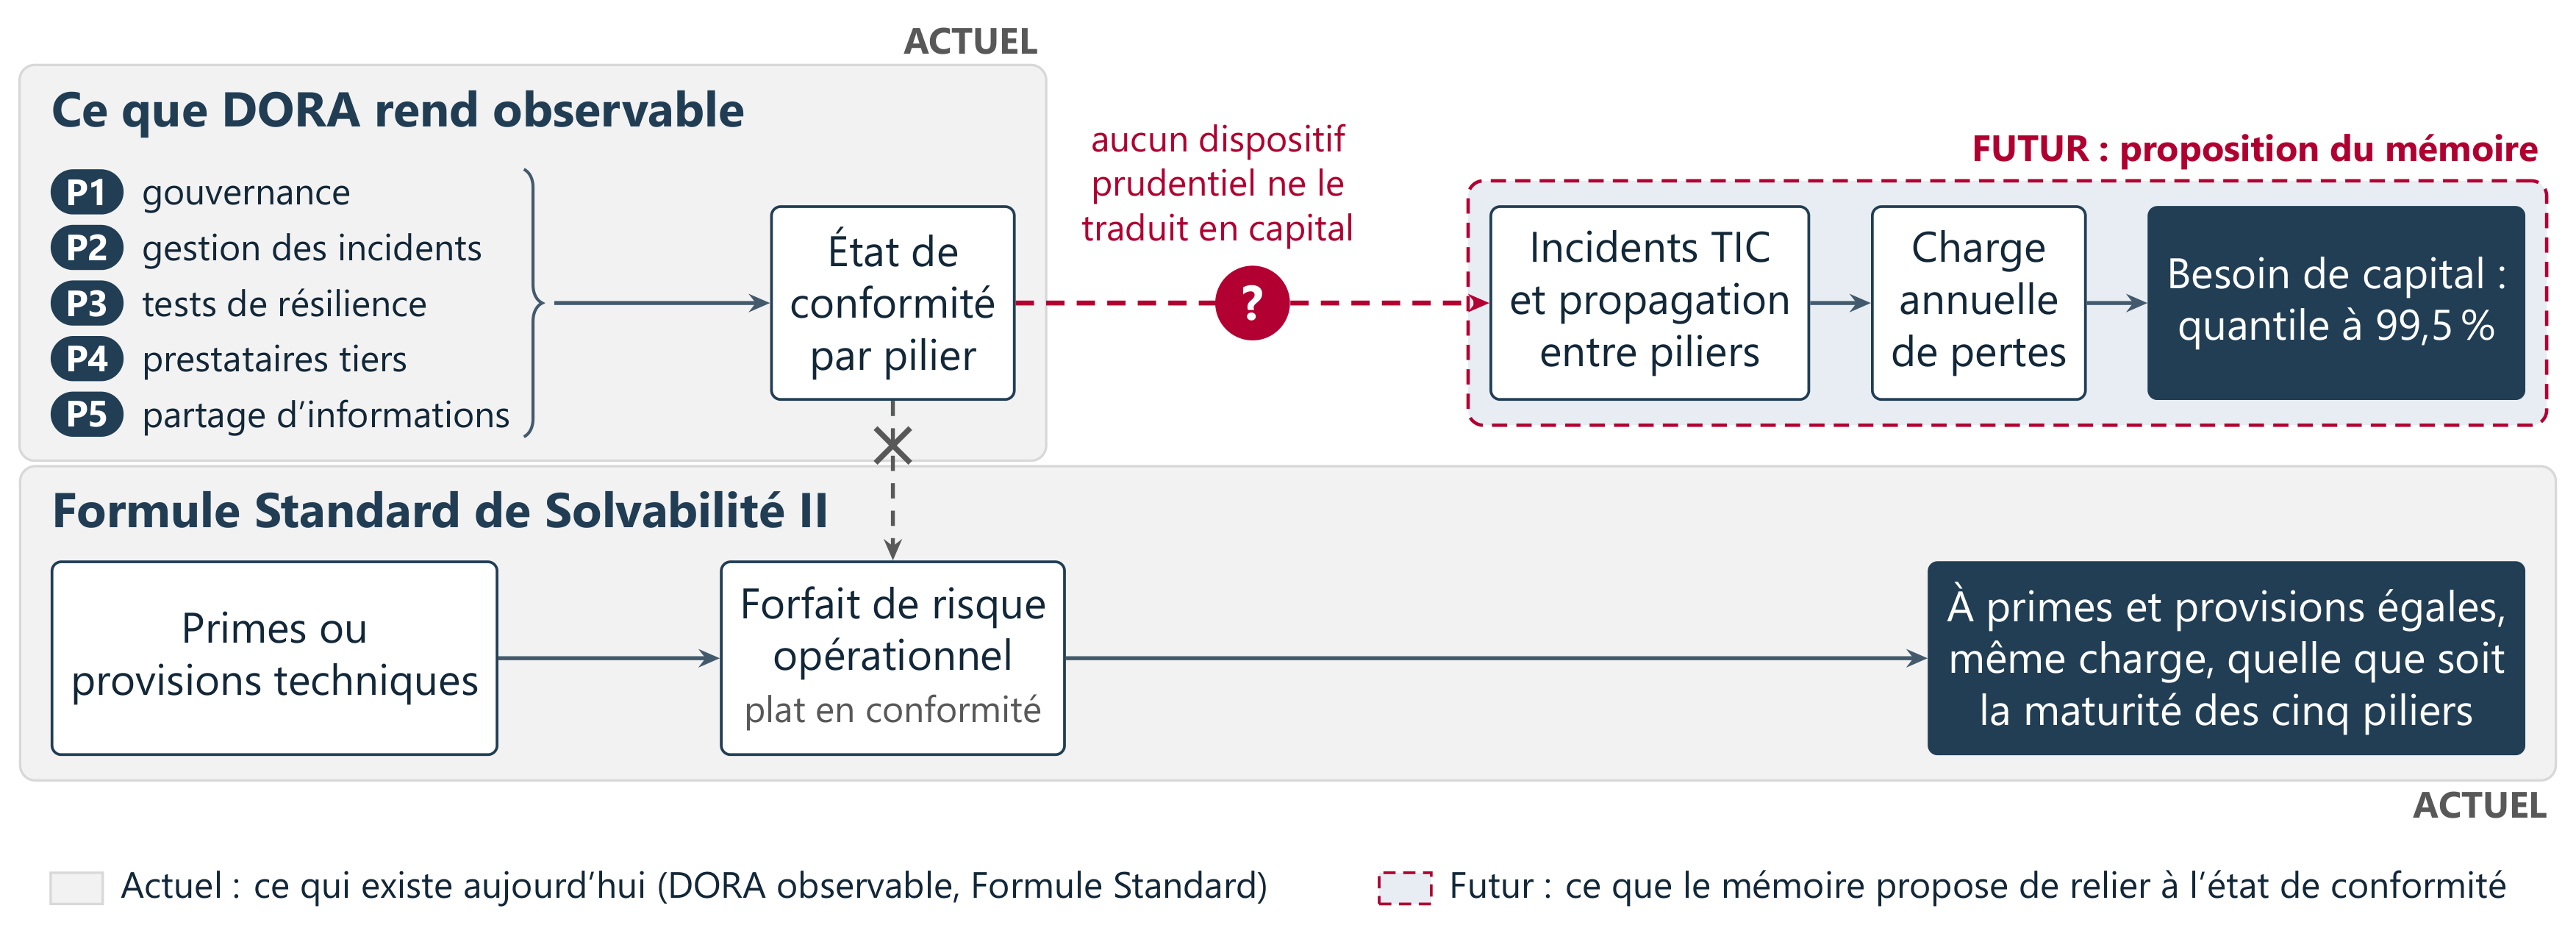
\includegraphics[width=0.90\textwidth]{schema_probleme.png}\\[2mm]
  {\small\color{ardoise}\bfseries Que coûte en capital un défaut de conformité,\\ indépendamment de l'état actuel d'une entité ?}
  \source{rapport, introduction et chapitre 1 (règlement DORA, cadre prudentiel).}
\end{frame}

\begin{frame}{Que prévoit DORA, pilier par pilier ?}
  \suivimethode{1}{État}
  \framesubtitle{\etabli Cinq domaines notés P1 à P5 · applicable depuis le 17 janvier 2025}
  \scriptsize
  \renewcommand{\arraystretch}{1.12}
  \begin{tabularx}{\linewidth}{@{}>{\bfseries}l l Y r@{}}
    \toprule
    Pilier & Articles & Exigence retenue & \shortstack[r]{Part d'amorce\\du modèle} \\
    \midrule
    P1 Gouvernance TIC & 5 à 16 & Responsabilité non délégable de l'organe de direction, cartographie des dépendances, contrôle interne & 30\,\% \\
    \rowcolor{clair}P2 Gestion des incidents & 17 à 23 & Notification sous 4 h après classification majeure (24 h au plus tard), rapport intermédiaire sous 72 h, final sous un mois & 18\,\% \\
    P3 Tests de résilience & 24 à 27 & Tests de pénétration guidés par la menace (TLPT) au moins tous les trois ans (art. 26) & 15\,\% \\
    \rowcolor{clair}P4 Prestataires tiers & 28 à 44 & Registre d'informations, clauses impératives (art. 30), stratégie de sortie, surveillance des prestataires critiques & 27\,\% \\
    P5 Partage d'informations & 45 & Partage volontaire et encadré : le pilier le moins utilisable dans un calibrage actuariel & 9\,\% \\
    \bottomrule
  \end{tabularx}
  \vspace{1.5mm}
  \begin{columns}[T,onlytextwidth]
    \column{.47\textwidth}\footnotesize
    Les piliers ne sont pas indépendants : un incident sur l'un dégrade la capacité de l'entité à tenir les autres. Le modèle formalise cette dépendance dirigée.
    \column{.49\textwidth}\footnotesize
    En 2025, 27 des 31 incidents majeurs notifiés à l'AMF (87\,\%) viennent d'un prestataire. Cette part dit d'où viennent les incidents, pas avec quelle probabilité ils passent d'un pilier à l'autre.
  \end{columns}
  \source{rapport, chapitre 1 (§ 1.4) et chapitre 5 (parts d'amorce proportionnelles au barème ROOT, posé à dire d'expert).}
\end{frame}

\begin{frame}{Quels incidents réels illustrent la propagation ?}
  \suivimethode{}{}
  \framesubtitle{\etabli Quatre cas publics, quatre hypothèses mises en défaut}
  \begin{columns}[T,onlytextwidth]
    \column{.235\textwidth}
    {\editorial\normalsize WannaCry, 2017}\par\vspace{.5mm}
    {\scriptsize\color{accent}\textbf{La propagation}}\par\vspace{1mm}
    \footnotesize Un rançongiciel auto-propagable exploite une faille de partage de fichiers et touche en quelques jours des organisations de dizaines de pays.\par\vspace{.8mm}
    {\scriptsize Onze mois plus tard, plus de 64 millions de tentatives sont encore bloquées en Russie : l'exposition est commune. Ce ne sont pas des sinistres.\par}
    \column{.235\textwidth}
    {\editorial\normalsize NotPetya, 2017}\par\vspace{.5mm}
    {\scriptsize\color{accent}\textbf{Le prestataire}}\par\vspace{1mm}
    \footnotesize La mise à jour d'un logiciel comptable ukrainien paralyse des groupes pendant des semaines.\par\vspace{.8mm}
    {\scriptsize L'incident naît chez un tiers (P4), se propage faute de cloisonnement (P1) et met la gestion de crise à l'épreuve (P2).\par}
    \column{.235\textwidth}
    {\editorial\normalsize MOVEit, 2023}\par\vspace{.5mm}
    {\scriptsize\color{accent}\textbf{L'accumulation}}\par\vspace{1mm}
    \footnotesize Une faille d'un logiciel de transfert de fichiers permet de dérober des données chez des milliers d'organisations.\par\vspace{.8mm}
    {\scriptsize Une défaillance tierce produit de nombreux sinistres simultanés ; nous l'utilisons comme expérience naturelle (chapitre 7).\par}
    \column{.235\textwidth}
    {\editorial\normalsize CrowdStrike, 2024}\par\vspace{.5mm}
    {\scriptsize\color{accent}\textbf{La dépendance sans adversaire}}\par\vspace{1mm}
    \footnotesize Une mise à jour défectueuse bloque des millions de postes dans le transport aérien, la banque et la santé.\par\vspace{.8mm}
    {\scriptsize Dépendance à un prestataire (P4) et absence de déploiement progressif (P3) : DORA couvre ce périmètre.\par}
  \end{columns}
  \vspace{1.5mm}
  {\color{filet}\rule{\linewidth}{.35pt}}\par\vspace{1.5mm}
  \begin{columns}[T,onlytextwidth]
    \column{.56\textwidth}\footnotesize
    \textbf{Structure commune.} Un incident naît sur un domaine de contrôle et en dégrade d'autres, dans un ordre. Aucune mesure de dépendance symétrique ne la restitue.
    \column{.40\textwidth}\footnotesize
    Vu de l'extérieur : l'attaque indirecte par un tiers pèse 35\,\% des vecteurs cités, 43\,\% dans les grandes entreprises (CESIN 2026).
  \end{columns}
  \source{rapport, chapitre 1 (§ 1.1.3 et § 1.5.1). Avast Threat Labs (2018) ; OpinionWay pour le CESIN (2026).}
\end{frame}

\begin{frame}{Que dit le marché français de la cyberassurance ?}
  \suivimethode{}{}
  \framesubtitle{\etabli Étude LUCY de l'AMRAE, édition 2026 (exercice 2025), analyse actuarielle co-écrite par le cabinet}
  \begin{columns}[T,onlytextwidth]
    \column{.50\textwidth}
    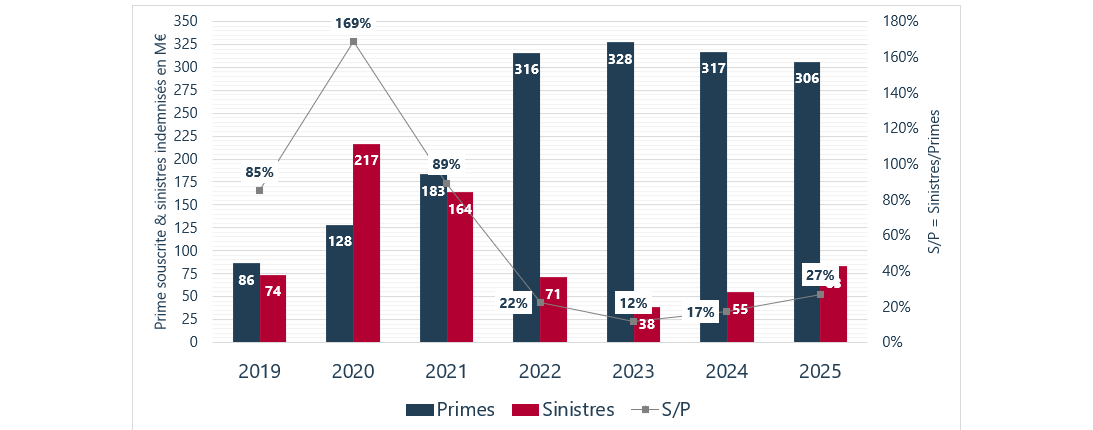
\includegraphics[width=\linewidth]{lucy_primes_sinistres_ratio.png}\par
    {\tiny\color{gris}Primes, sinistres indemnisés et ratio sinistres sur primes, 2019--2025 (citation externe, non recalculable).\par}
    \column{.47\textwidth}\footnotesize
    \textbf{83,2 M€} indemnisés en 2025 contre 54,5 en 2024 (+53\,\%), sur 20\,996 polices et 1\,251 sinistres. Le ratio sinistres sur primes remonte de 12\,\% (2023) à 27\,\%, loin des 169\,\% de 2020.\par\vspace{2mm}
    \renewcommand{\arraystretch}{1.25}
    \begin{tabular}{@{}lrrr@{}}
      \toprule
      Marché & Nombre & Coût moyen & Charge \\
      \midrule
      Exercice 2024 & $\times 0{,}73$ & $\times 1{,}96$ & $\times 1{,}43$ \\
      Exercice 2025 & $\times 2{,}79$ & $\times 0{,}55$ & $\times 1{,}53$ \\
      \bottomrule
    \end{tabular}\par\vspace{2mm}
    Une même hausse du ratio recouvre deux régimes opposés : en 2024 la sévérité, en 2025 le nombre de sinistres.\par\vspace{1.5mm}
    \textcolor{accent}{\textbf{Un seul sinistre dépasse 10 M€ en 2025.}} L'historique national s'arrête avant le haut de la distribution : la sévérité se calibre à l'international.
  \end{columns}
  \source{rapport, chapitre 1 (§ 1.3). La charge indemnisée est nette de franchise et plafonnée par la capacité : elle ne se compare pas à la perte brute d'une entité.}
\end{frame}

\begin{frame}{Que ne dit pas la Formule Standard du risque opérationnel ?}
  \suivimethode{}{}
  \framesubtitle{\etabli Un forfait sur les volumes, identique pour deux entités de même bilan}
  \begin{columns}[T,onlytextwidth]
    \column{.47\textwidth}
    {\small\textbf{Solvabilité II}\par}\vspace{.5mm}
    \footnotesize\setlength{\abovedisplayskip}{.5mm}\setlength{\belowdisplayskip}{.5mm}
    \[\mathrm{SCR}_{\mathrm{Op}}=\min(0{,}3\,\mathrm{BSCR},\ \mathrm{Op})+0{,}25\,\mathrm{Exp}_{\mathrm{ul}}\]
    $\mathrm{Op}=\max(\mathrm{Op}_{\text{primes}},\mathrm{Op}_{\text{provisions}})$ : coefficients forfaitaires sur les volumes ; le $\mathrm{SCR}_{\mathrm{Op}}$ s'ajoute au BSCR sans diversification.\par\vspace{1.5mm}
    {\small\textbf{Bâle}\par}\vspace{.5mm}
    Les modèles internes (AMA) sont retirés du calcul du capital depuis le 1\textsuperscript{er} janvier 2025 ; la méthode standardisée applique $\mathrm{ORC}=\mathrm{BIC}\times\mathrm{ILM}$. La distribution des pertes (LDA) reste un outil de modélisation : nous en gardons les marges de fréquence et de sévérité.
    \column{.49\textwidth}\scriptsize
    \renewcommand{\arraystretch}{1.1}
    \begin{tabularx}{\linewidth}{@{}>{\bfseries}l Y Y@{}}
      \toprule
      & ORSA & DORA \\
      \midrule
      Taxonomie & Agrégée dans le module $\mathrm{SCR}_{\mathrm{Op}}$ & Actifs TIC granulaires \\
      Incidents & Notification interne non standardisée & Notification à l'autorité : 4 h, 72 h, un mois \\
      Tests & Stress tests de capital & Continuité et TLPT tous les trois ans \\
      Dépendances & Accords d'externalisation généraux & Registre harmonisé, chaînes de sous-traitance \\
      Tiers & Lignes directrices non contraignantes & Clauses impératives, surveillance directe \\
      \bottomrule
    \end{tabularx}
  \end{columns}
  \vspace{1.5mm}
  {\color{accent}\small\textbf{Le vide que le travail comble.}} \footnotesize DORA rend observable un niveau de maîtrise qui ne l'était pas, mais aucun dispositif prudentiel ne le traduit en capital. Nous le traduisons dans l'ORSA, seul cadre qui admette des scénarios stochastiques.
  \source{rapport, chapitre 1 (§ 1.5.2 et § 1.6). Aucun module DORA n'existe en Formule Standard : la grandeur calculée est un besoin de capital ORSA, pas un SCR réglementaire.}
\end{frame}

\begin{frame}{Pourquoi retenir un quantile à 99,5\,\% ?}
  \framesubtitle{\etabli Un repère annuel cohérent avec Solvabilité II ; un niveau incertain}
  \[B=\VaR_{99{,}5\%}(L),\qquad L=\sum_{n=1}^{N}X_n.\]
  \begin{center}\footnotesize $N$ : nombre d'incidents sur un an ; $X_n$ : perte de l'incident $n$ ; $L$ : perte annuelle.\end{center}
  \vspace{3mm}
  \begin{columns}[T]
    \column{.30\textwidth}
    {\editorial\normalsize Le choix}\par\vspace{2mm}
    \footnotesize Un montant dépassé dans 0,5\,\% des années du modèle.\par\vspace{2mm}
    Besoin de capital au sens de l'ORSA, distinct du SCR réglementaire complet.
    \column{.30\textwidth}
    {\editorial\normalsize La vérification}\par\vspace{2mm}
    \footnotesize Détecter un taux de dépassement doublé demanderait 1\,811 années.\par\vspace{2mm}
    Le backtest disponible ne valide pas ce quantile extrême.
    \column{.30\textwidth}
    {\editorial\normalsize La limite}\par\vspace{2mm}
    \footnotesize L'incertitude sur les pertes extrêmes multiplie par 2,5 la plage du quantile d'un sinistre.\par\vspace{2mm}
    Le niveau doit être accompagné de sa sensibilité.
  \end{columns}
  \question{Que sait-on déjà modéliser, et que manque-t-il ?}
  \source{rapport, chapitres 4, 9 et 10. VaR : Value at Risk, quantile de perte. ORSA : évaluation interne des risques et de la solvabilité. SCR : capital de solvabilité requis.}
\end{frame}

\begin{frame}{Que propose déjà la littérature, et que lui manque-t-il ?}
  \framesubtitle{Travaux existants et propriétés d'une dépendance entre domaines de contrôle}
  \centering\scriptsize\vspace*{-3mm}
  \renewcommand{\arraystretch}{1.0}
  \setlength{\tabcolsep}{3pt}
  \begin{tabular}{@{}c >{\raggedright\arraybackslash}p{0.285\textwidth} *{5}{>{\centering\arraybackslash}p{0.108\textwidth}}@{}}
    \toprule
    & & \cc{\textbf{Statique}} & \multicolumn{4}{c}{\textbf{Contagion dirigée}} \\
    \cmidrule(lr){3-3}\cmidrule(lr){4-7}
    \textbf{Famille} & \textbf{Travaux} & \cc{\textbf{Dépendance des pertes}} & \cc{\textbf{Direction}} & \cc{\textbf{Ordre d'atteinte}} & \cc{\textbf{Cycles de $W$}} & \cc{\textbf{Propagation}} \\
    \midrule
    \multirow{2}{*}{\raisebox{0pt}[0pt][0pt]{\rotatebox[origin=c]{90}{\textbf{Copules}}}}
      & \auteur{Böhme et Kataria (2006)} & \ck{Copule} & & & & \\
      & \auteur{Herath et Herath (2011)} & \ck{Copule} & & & & \\
    \midrule
    \multirow{4}{*}{\raisebox{0pt}[0pt][0pt]{\rotatebox[origin=c]{90}{\textbf{Dynamique}}}}
      & \auteur{Hillairet et Lopez (2021)} & & \ck{Réseau d'entités} & & \ck{Boucles admises} & \ck{SIR, états} \\
      & \auteur{Hillairet, Lopez et al. (2022)} & & \ck{Réseau d'entités} & & \ck{Boucles admises} & \ck{SIR, portefeuille} \\
      & \auteur{Bessy-Roland et al. (2021)} & & \ck{Types d'attaque} & & \ck{Boucles admises} & \ck{Auto-excitation} \\
      & \auteur{Boumezoued et al. (2023)} & & \ck{Types d'attaque} & & \ck{Boucles admises} & \ck{Excitation ext.} \\
    \midrule
    \multirow{1}{*}{\raisebox{0pt}[0pt][0pt]{\rotatebox[origin=c]{90}{\textbf{Ici}}}}
      & \begin{tabular}[c]{@{}l@{}}\textbf{Ce travail (2026)}\end{tabular} & \ckr{Part $S$} & \ckr{Modélisée} & \ckr{Ordonnés} & \ckr{Admis dans $W$} & \ckr{Entre piliers} \\
    \bottomrule
  \end{tabular}
  \par\vspace{0.3mm}
  {\tiny\color{gris}\textit{Ordre d'atteinte} : suite des piliers touchés par un incident.
  \textit{Cycles de $W$} : boucles admises dans le graphe ; le moteur de capital suit une marche auto-évitante, arrêtée au retour sur un pilier touché.\par}
  \vspace{0.4mm}
  {\footnotesize\color{ardoise}\bfseries Parmi les travaux comparés, seule la cascade dirigée modélise les quatre colonnes entre piliers d'une entité ; sa direction est modélisée, non identifiée, puis bornée.}\\[0.4mm]
  {\tiny\color{gris}Ce que nous reprenons : marges empiriques et risque extrême (copules) ; états successifs (Hillairet et Lopez) ; test sur nos données, non distinguable de la cascade (Hawkes).}
  \source{rapport, chapitre 2 (tableau de comparaison, section « Comparaison aux approches existantes ») ; comparaison détaillée en annexe B.}
\end{frame}


% =============================================================================
\section{Données}
\begin{frame}{De quelles données disposons-nous, et que permettent-elles ?}
  \framesubtitle{La fréquence et la sévérité des pertes extrêmes, pas la direction de la contagion}
  \begin{columns}[T]
    \column{0.70\textwidth}
    \scriptsize
    \renewcommand{\arraystretch}{1.3}
    \begin{tabularx}{\linewidth}{>{\hsize=0.85\hsize}Y >{\hsize=1.0\hsize}Y >{\hsize=1.1\hsize}Y >{\hsize=1.05\hsize}Y}
      \toprule
      \textbf{Source} & \textbf{Effectif retenu} & \textbf{Rôle dans le modèle} & \textbf{Biais et limites} \\
      \midrule
      \textbf{SAS OpRisk Global} & 41\,975 pertes, dont 582 cyber × finance & Sévérité en euros ; fréquence d'entrée du moteur & Sélection : biais vers les grandes entités \\
      \rowcolor{clair}\textbf{Chronologie PRC} & 15\,053 incidents, 2019 à 2025 & Fréquence de référence, sans rôle de niveau & Mesure : sévérité dérivée d'un modèle log-log \\
      \textbf{Hackmageddon} & 1\,041 incidents, premier semestre 2026 & Parts par vecteur d'attaque & Déclaration : incidents publics, taxonomie instable \\
      \bottomrule
    \end{tabularx}\\[3mm]
    \small Le niveau de fréquence est lu sur OpRisk, la répartition par vecteur d'attaque sur Hackmageddon.
    Aucune de ces sources ne dit quel pilier a entraîné l'autre : la direction de la contagion n'y est pas observée.
    \question{Comment relier ces pertes à l'état de conformité de chaque pilier ?}
    \column{0.26\textwidth}
    \chiffre{91 excès}{au-delà du seuil $u$, sur les 582 pertes cyber × finance du rapport ; sur la seule période 2000--2026 : 86 excès sur 570, mêmes $\xi$ et $\sigma$}
    \vspace{4mm}
    \chiffre{1 sinistre}{au-delà de 10\Meur sur le marché français en 2025 : la sévérité se calibre sur une base internationale}
  \end{columns}
  \source{rapport, chapitre 3 ; chapitre 1, figure 1.1. Population de calibration : script 129.}
\end{frame}

\begin{frame}{Quels biais, et que corrige-t-on ?}
  \suivimethode{3,4}{Fréquence, sévérité}
  \framesubtitle{\etabli Sélection, déclaration, troncature, dérive nominale}
  \begin{columns}[T,onlytextwidth]
    \column{.60\textwidth}\scriptsize
    \renewcommand{\arraystretch}{1.12}
    \begin{tabularx}{\linewidth}{@{}>{\bfseries}l Y Y@{}}
      \toprule
      Biais & Mécanisme & Traitement \\
      \midrule
      Sélection (OpRisk) & Pertes rendues publiques : grandes entités, montants exceptionnels & Fréquence et sévérité ramenées à la taille par deux élasticités estimées \\
      \rowcolor{clair}Déclaration (PRC) & Fuites de données obligatoires, pas les rançongiciels sans exfiltration & Niveau lu sur OpRisk, répartition par vecteur sur Hackmageddon \\
      Troncature à droite & 97 événements observés en 2023--2025, 255 à l'ultime (chain-ladder) & Fréquence relevée d'un facteur 1,147 : 85,0 par an contre 74,1 \\
      \rowcolor{clair}Dérive nominale & Rapport nominal sur courant de 1,747 en 2004 : inflation implicite de 2,19\,\% par an & Calibration sur montants nominaux, effet mesuré au backtest \\
      Survie & Entités disparues sous-représentées & Ni existence ni signe établis : non chiffré \\
      \bottomrule
    \end{tabularx}
    \column{.36\textwidth}\footnotesize
    {\editorial\normalsize Deux corrections qui se compensent presque}\par\vspace{1.5mm}
    Sévérité transposée à l'entité : $\times\,0{,}861$ ; fréquence : $\times\,1{,}147$. Le produit vaut $0{,}987$, soit $1{,}3\,\%$ d'effet net sur la perte moyenne.\par\vspace{1.5mm}
    {\color{accent}Mais pas sur le capital :} à queue lourde, le quantile à 99,5\,\% répond à la sévérité bien plus qu'à la fréquence.\par\vspace{3mm}
    {\editorial\normalsize Chronologie PRC}\par\vspace{1.5mm}
    Volume touché renseigné dans $41{,}77\,\%$ des cas (champ \texttt{UNKN} compté comme manquant) ; la déduplication retire 1\,643 lignes, soit $10{,}9\,\%$, borne basse.
  \end{columns}
  \source{rapport, chapitre 3 (§ 3.2, 3.3, 3.5 et 3.8).}
\end{frame}

\begin{frame}{Pourquoi retenir une queue commune ?}
  \suivimethode{4}{Sévérité}
  \framesubtitle{\etabli Ni la catégorie ni la taille ne segmentent la queue}
  \begin{columns}[T,onlytextwidth]
    \column{.34\textwidth}\footnotesize
    {\editorial\normalsize Forme de la sévérité}\par\vspace{1.5mm}
    \renewcommand{\arraystretch}{1.12}
    \begin{tabular}{@{}lr@{}}
      \toprule
      Médiane & 1,20 M\$ \\
      Moyenne & 33,8 M\$ \\
      P90 & 25,3 M\$ \\
      P99 & 419,3 M\$ \\
      Maximum & 10\,970,8 M\$ \\
      Total cumulé & 49,8 Md\$ \\
      \bottomrule
    \end{tabular}\par\vspace{1.5mm}
    Le décile supérieur concentre $92{,}3\,\%$ de la perte totale, le centile supérieur $65{,}1\,\%$.
    \column{.62\textwidth}\footnotesize
    {\editorial\normalsize Trois instruments, une conclusion}\par\vspace{1.5mm}
    \renewcommand{\arraystretch}{1.12}
    \begin{tabularx}{\linewidth}{@{}>{\bfseries}l Y@{}}
      \toprule
      $V$ de Cramér & Sous $0{,}20$ pour les cinq associations ; la plus forte, la catégorie bâloise, vaut $0{,}176$ \\
      $\varepsilon^2$ de Kruskal-Wallis & De $0{,}0100$ à $0{,}0785$ : la classe explique entre un et huit pour cent de la dispersion \\
      Corrélation de rang & Perte contre chiffre d'affaires $0{,}159$, effectif $0{,}139$, actif total $0{,}068$ sur $33\,769$ pertes \\
      \bottomrule
    \end{tabularx}\par\vspace{2mm}
    Segmenter par la catégorie bâloise (sept modalités) ramènerait les 86 excès à une douzaine par modalité : aucune loi de queue ne s'y ajuste. Nous ajustons donc \textbf{une queue commune}, hypothèse qui repose sur des tailles d'effet mesurées.\par\vspace{2mm}
    {\scriptsize L'actif total, qui porte la mise à l'échelle prudentielle, est la mesure de taille la moins liée à la perte : ce constat motive la lecture de la taille au chapitre 9.\par}
  \end{columns}
  \source{rapport, chapitre 3 (§ 3.7 et 3.8). Population de fréquence : secteur financier, catégories TIC, 2005--2022, 1\,476 observations.}
\end{frame}

\begin{frame}{Que fixe Hackmageddon, et que ne fixe-t-il pas ?}
  \suivimethode{3}{Fréquence}
  \framesubtitle{\etabli La structure du risque par vecteur d'attaque, jamais son niveau}
  \begin{columns}[T,onlytextwidth]
    \column{.55\textwidth}\footnotesize
    \renewcommand{\arraystretch}{1.1}
    \begin{tabularx}{\linewidth}{@{}Y r Y@{}}
      \toprule
      \textbf{Vecteur d'attaque} & \textbf{Part} & \textbf{Exigence DORA} \\
      \midrule
      Hameçonnage & 38,8\,\% & Art. 13, formation \\
      \rowcolor{clair}Exploitation de vulnérabilité & 33,8\,\% & Art. 26 (TLPT), art. 8 à 10 \\
      Chaîne d'approvisionnement & 15,8\,\% & Art. 28 à 44, risque tiers \\
      \rowcolor{clair}Identifiants compromis & 6,3\,\% & Art. 9, authentification forte \\
      Autres & 5,3\,\% & --- \\
      \bottomrule
    \end{tabularx}\par\vspace{2mm}
    49,6\,\% des attaques, dont les 15,8\,\% du vecteur tiers, relèvent de vecteurs qu'un test TLPT est censé détecter en amont.
    \column{.41\textwidth}\footnotesize
    {\editorial\normalsize Un statut de citation datée}\par\vspace{1.5mm}
    Semestre de janvier à juin 2026 : 1\,041 incidents, dont 840 à vecteur d'accès initial identifié (81\,\%).\par\vspace{1.5mm}
    Le jeu consulté n'a pas été conservé ; relu en octobre 2026 avec une autre grille, il ne redonne pas ces décomptes à l'unité.\par\vspace{1.5mm}
    La taxonomie est instable : une lecture naïve prête au rançongiciel une hausse de 11 points là où, après reclassement, il recule de 23.\par\vspace{1.5mm}
    {\color{accent}Le multiplicateur de fréquence hérite de ce statut.}
  \end{columns}
  \source{rapport, chapitre 3 (§ 3.6). Les parts pondèrent le multiplicateur de fréquence entre états ; elles ne fixent aucun nombre d'incidents.}
\end{frame}

\begin{frame}{Quelle fréquence entre dans le moteur ?}
  \suivimethode{3}{Fréquence}
  \framesubtitle{\etabli Trois taux, trois niveaux d'observation : un seul porte le capital}
  \begin{columns}[T,onlytextwidth]
    \column{.64\textwidth}\footnotesize
    \renewcommand{\arraystretch}{1.1}
    \begin{tabularx}{\linewidth}{@{}>{\bfseries}l l r Y@{}}
      \toprule
      Taux & Source & Valeur & Ce qu'il compte \\
      \midrule
      $\lambda_{\mathrm{ref}}$ & PRC & 341/an & Notifications de violations des organisations financières ; n'entre pas dans le moteur \\
      \rowcolor{clair}$\lambda$ & OpRisk & 21,6/an & Incidents TIC matériels du périmètre financier : \textcolor{accent}{entrée du moteur}, seul taux dont dépend le capital \\
      $\lambda_{\mathrm{entité}}$ & OpRisk & 0,092/an & Événements du panel rapportés à une firme, lus à la taille de l'entité notionnelle \\
      \bottomrule
    \end{tabularx}\par\vspace{2mm}
    Le facteur 3\,719 entre $\lambda_{\mathrm{ref}}$ et $\lambda_{\mathrm{entité}}$ sépare trois comptages : notifications, pertes matérielles du secteur, pertes matérielles par entité.
    \column{.32\textwidth}\footnotesize
    {\editorial\normalsize Un écart déclaré}\par\vspace{1.5mm}
    La fréquence gelée vaut $582/27 = 21{,}56$ ; l'échantillon de sévérité donne $570/27 = 21{,}11$, soit $2{,}1\,\%$ de moins.\par\vspace{1.5mm}
    Le numérateur compte douze pertes d'avant 2000 et le dénominateur de 27 ans inclut 2026, année incomplète : le sens de l'écart de niveau n'est pas établi. Nous le déclarons sans corriger la valeur.
  \end{columns}
  \vspace{1mm}
  \footnotesize\textbf{Surdispersion.} Pour un mélange de Poisson, l'indice vaut $1+\lambda/r$ : il croît avec le niveau de lecture. Il est de $1{,}19$ sur les cellules firme-année, de $2{,}24$ sur la série annuelle détendancée ; le moteur retient $9{,}20$, choix de prudence.
  \source{rapport, chapitre 3 (§ 3.4) et chapitre 4 (§ 4.3).}
\end{frame}


% =============================================================================
\section{Fréquence-sévérité}
\begin{frame}{Comment modéliser des pertes rares et concentrées ?}
  \framesubtitle{\etabli Comptage annuel et montant d'un sinistre : deux objets distincts}
  \begin{columns}[T,onlytextwidth]
    \column{.32\textwidth}\small
    \textbf{Comptage}\par
    Binomiale négative : une dispersion supérieure à Poisson.\par\vspace{4mm}
    \textbf{Pertes extrêmes}\par
    GPD ajustée à 91 excès au-delà de 20,03 M€ ; sur 2000--2026 (86 excès), mêmes paramètres.\par\vspace{4mm}
    \textbf{Paramètres}\par
    $\xi=0{,}595$ : forme.\par
    $\sigma=57{,}97$ M€ : échelle.
    \column{.64\textwidth}
    \begin{minipage}[t]{.49\linewidth}\centering
      {\scriptsize\bfseries Vie résiduelle moyenne $e(v)$, M€\\[-.3mm]\mdseries linéaire au-delà de $u$\par}\vspace{.5mm}
      \adjustbox{trim={.1\width} 0pt 0pt {.22\height},clip,width=\linewidth}{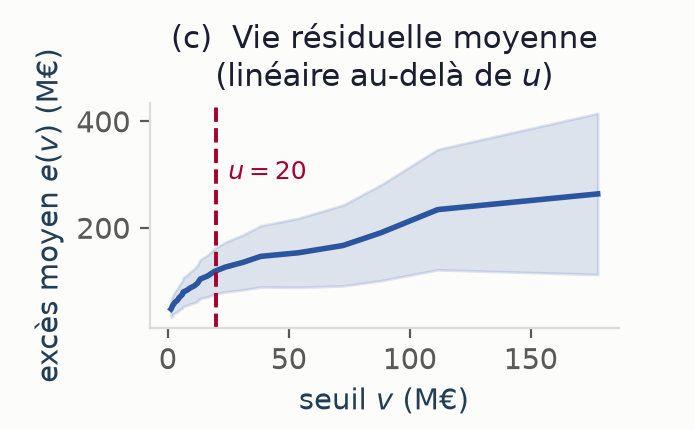
\includegraphics{j3_c.png}}
    \end{minipage}\hfill
    \begin{minipage}[t]{.49\linewidth}\centering
      {\scriptsize\bfseries Stabilité de $\hat\xi$ au seuil\\[-.3mm]\mdseries intervalle à 90\,\%\par}\vspace{.5mm}
      \adjustbox{trim=0pt 0pt 0pt {.165\height},clip,width=\linewidth}{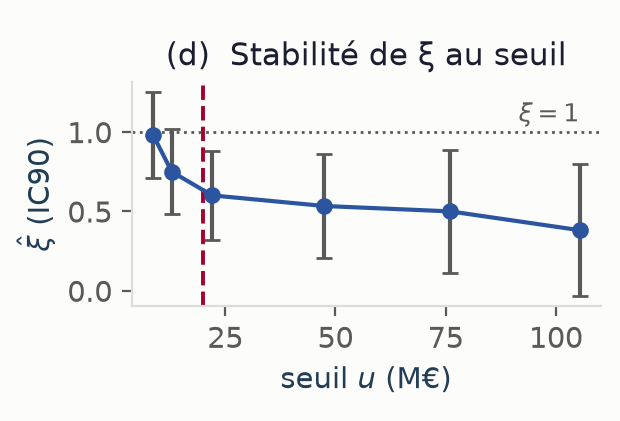
\includegraphics{j3_d.png}}
    \end{minipage}\par\vspace{3mm}
    \small\textcolor{accent}{\textbf{663 M€}} : quantile à 99,5\,\% d'un sinistre, \textbf{pas un capital annuel}.\par
    Sensibilité : [411 ; 1\,037] M€.
  \end{columns}
  \question{Où placer le seuil qui sépare le corps de la queue ?}
  \source{rapport, chapitre 4 ; population de calibration : script 129. Intervalle historique à 90\,\%. Le quantile d'un sinistre n'est pas le capital annuel.}
\end{frame}

\begin{frame}{Pourquoi une loi de Pareto généralisée ?}
  \suivimethode{4}{Sévérité}
  \framesubtitle{\etabli Deux théorèmes d'extrapolation de queue}
  \begin{columns}[T,onlytextwidth]
    \column{.52\textwidth}\scriptsize
    \setlength{\abovedisplayskip}{.5mm}\setlength{\belowdisplayskip}{.5mm}
    \textbf{Fisher--Tippett--Gnedenko.} Si le maximum normalisé converge, la limite est une loi des valeurs extrêmes $H_\xi$ : Fréchet ($\xi>0$, queue lourde), Gumbel ($\xi=0$) ou Weibull ($\xi<0$, support borné).\par\vspace{.8mm}
    \textbf{Pickands--Balkema--de Haan.} Les excès au-delà d'un seuil $u$ convergent vers une GPD $G_{\xi,\sigma}$ de même indice $\xi$ : toutes les pertes au-delà de $u$ servent, non un maximum par bloc.
    \[q_\alpha(X)=u+\frac{\sigma}{\xi}\Big[\Big(\frac{1-\alpha}{\zeta_u}\Big)^{-\xi}-1\Big],\qquad \zeta_u=\mathbb P(X>u)\]
    Calibration OpRisk : $u=20{,}03$, $\sigma=57{,}97$, $\xi=0{,}595$, $\zeta_u=0{,}151$.\par\vspace{.8mm}
    \textcolor{accent}{\textbf{663,0 M€}} : quantile à 99,5\,\% d'un sinistre ; \textcolor{accent}{\textbf{1\,752,4 M€}} : sa moyenne de queue. Ni l'un ni l'autre n'est un capital.\par\vspace{.8mm}
    Variance infinie dès $\xi\ge 1/2$, espérance infinie dès $\xi\ge 1$ : ici, variance infinie, espérance finie. Intervalle à 90\,\% de $\xi$ : $[0{,}320\,;0{,}871]$ par delta-méthode, $[0{,}304\,;0{,}831]$ par bootstrap.
    \column{.44\textwidth}
    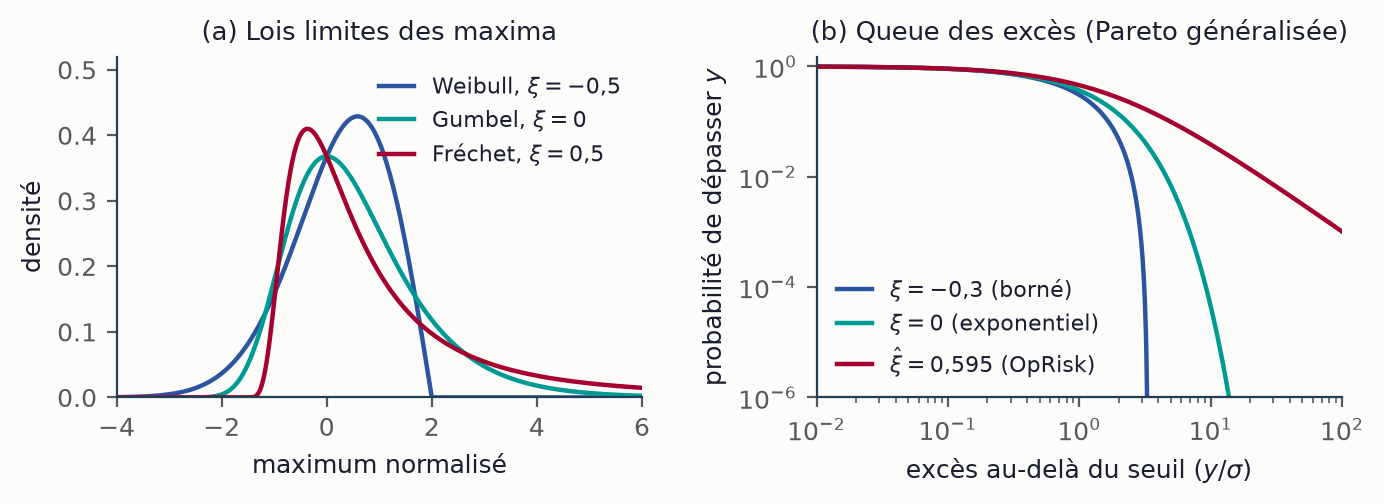
\includegraphics[width=\linewidth]{GEV_domaines_attraction.png}\par
    {\tiny\color{gris}(a) densités des lois de valeurs extrêmes, valeurs d'illustration. (b) probabilité qu'un excès dépasse $y$ : décroissance exponentielle à $\xi=0$, en puissance à l'indice calibré.\par}
  \end{columns}
  \source{rapport, chapitre 4 (§ 4.1, 4.2, figure 4.1) ; démonstrations en annexe B du rapport.}
\end{frame}

\begin{frame}{Du quantile d'un sinistre au capital annuel}
  \suivimethode{6,7}{Perte, capital}
  \framesubtitle{\etabli q pour un sinistre, VaR pour la charge annuelle}
  \begin{columns}[T,onlytextwidth]
    \column{.46\textwidth}\footnotesize
    \setlength{\abovedisplayskip}{.5mm}\setlength{\belowdisplayskip}{.5mm}
    \textbf{Un sinistre}
    \[\mathrm q_{99{,}5\,\%}(X)=663\ \text{M€}\]
    Dépassé une fois sur deux cents par un sinistre isolé.\par\vspace{1.5mm}
    \textbf{Une année}
    \[L=\sum_{n=1}^{N}X_n,\quad \mathrm{VaR}_{99{,}5\,\%}(L)=8\,123\ \text{M€}\]
    Dépassée une année sur deux cents, pour le périmètre financier étudié (sévérité OpRisk).\par\vspace{1.5mm}
    {\scriptsize Le pont : à $\lambda\simeq 21{,}6$ sinistres par an, atteindre le quantile annuel à 99,5\,\% suppose un quantile par sinistre de l'ordre de $99{,}98\,\%$. Le sens de l'inégalité s'inverse avec l'échelle : comparer 663 et 8\,123 ne conclut jamais.\par}
    \column{.50\textwidth}\footnotesize
    \textbf{Contrôle sans simulation}\par\vspace{1mm}
    La charge annuelle est une somme composée : son quantile se calcule par inversion de Fourier de sa fonction génératrice, méthode distincte de la récursion de Panjer.\par\vspace{1.5mm}
    \renewcommand{\arraystretch}{1.1}
    \begin{tabular}{@{}lrr@{}}
      \toprule
      Capital, M€ & Conforme & Non conforme \\
      \midrule
      Monte-Carlo & 6\,049 & 20\,188 \\
      Inversion de Fourier & 5\,945 & 19\,890 \\
      \bottomrule
    \end{tabular}\par\vspace{1.5mm}
    L'écart vaut 0,75 et 0,59 erreur type de la référence simulée : il n'est pas résolu. L'approximation par perte unique reste à moins de dix pour cent au second ordre.\par\vspace{1mm}
    {\color{accent}Le contrôle vérifie l'agrégation, pas la vérité du modèle.}
  \end{columns}
  \source{rapport, chapitre 4 (§ 4.2) et chapitre 10 (§ 10.4). VaR et TVaR sont réservées à la charge annuelle ; q et $\bar{\mathrm q}$ au sinistre.}
\end{frame}

\begin{frame}{La binomiale négative est-elle validée ?}
  \suivimethode{3}{Fréquence}
  \framesubtitle{\etabli Rejet du Poisson, meilleure couverture hors échantillon}
  \begin{columns}[T,onlytextwidth]
    \column{.50\textwidth}\scriptsize
    \renewcommand{\arraystretch}{1.1}
    \begin{tabularx}{\linewidth}{@{}>{\bfseries}l Y@{}}
      \toprule
      Rapport de vraisemblance & Rejette le Poisson : $130{,}5$, $p\approx 10^{-30}$ sur 14\,944 cellules firme-année (supposées indépendantes) \\
      \rowcolor{clair}Dispersion & $1{,}19$ (cellules), $2{,}24$ (série annuelle, IC à 95\,\% $[1{,}24\,;5{,}18]$), $9{,}20$ au moteur \\
      Backtest & Intervalle à 90\,\% : 11 années sur 12 ($91{,}7\,\%$) pour la binomiale négative, 9 sur 12 ($75{,}0\,\%$) pour le Poisson \\
      \rowcolor{clair}Log-score & $+3{,}054$ nats pour la binomiale négative, gain dû à trois années \\
      \bottomrule
    \end{tabularx}\par\vspace{1.5mm}
    Douze années donnent trop peu de puissance : le résultat va dans le sens du choix sans le démontrer, et ne teste pas la surdispersion posée au moteur.\par\vspace{1mm}
    Passer du Poisson à la binomiale négative relève le capital du secteur de $+9\,\%$ : le quantile reste porté par la perte unique dominante.
    \column{.46\textwidth}
    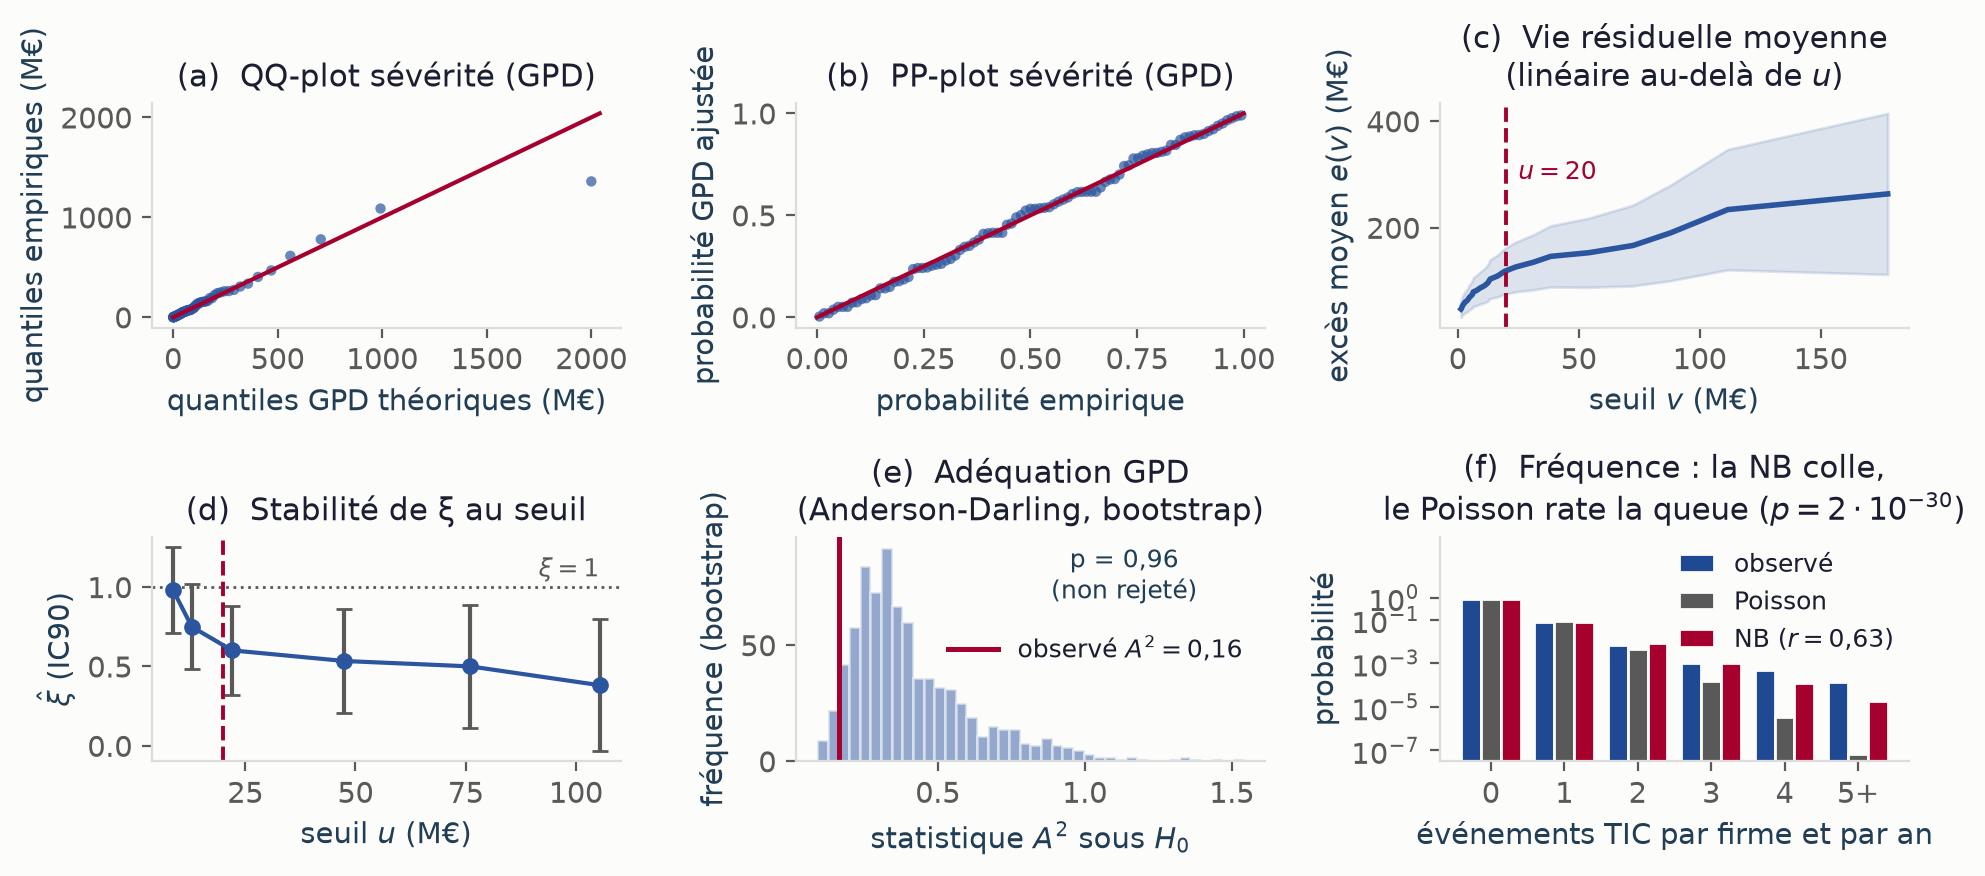
\includegraphics[width=\linewidth]{J3_validation_adequation.png}\par
    {\tiny\color{gris}(a-b) QQ et PP de la sévérité, (c) vie résiduelle moyenne, (d) stabilité de $\hat\xi$, (e) Anderson-Darling, (f) fréquence : la binomiale négative colle aux comptes, le Poisson rate la queue.\par}
  \end{columns}
  \source{rapport, chapitre 4 (§ 4.3, 4.6, 4.7, figure 4.2). Le facteur 9,20 est un choix de prudence sur la queue de fréquence.}
\end{frame}

\begin{frame}{Le modèle prédit-il l'année suivante ?}
  \suivimethode{4,7}{Sévérité, capital}
  \framesubtitle{\etabli Origine glissante 2004--2025, douze années notées}
  \begin{columns}[T,onlytextwidth]
    \column{.56\textwidth}\footnotesize
    \renewcommand{\arraystretch}{1.18}
    \begin{tabularx}{\linewidth}{@{}>{\bfseries}l Y@{}}
      \toprule
      Forme de la queue & Kolmogorov-Smirnov sur la probabilité intégrale des excès : $D=0{,}100$, $p=0{,}4087$ ; la GPD n'est pas rejetée \\
      \rowcolor{clair}Quantiles de sévérité & Kupiec rejette à 99\,\% ($p=0{,}0078$ ; 8 dépassements pour 2,8 attendus) et à 99,5\,\% ($p=0{,}0140$ ; 5 pour 1,4) \\
      Dérive d'échelle & $3{,}40\,\%$ par an dans la queue ($p=0{,}1786$), $3{,}30\,\%$ corrigée de l'inflation ; effet d'au moins $+16{,}9\,\%$ sur le quantile \\
      \rowcolor{clair}Facteur entre états & De $3{,}337$ à $3{,}164$ ($-5{,}2\,\%$) sous la sévérité dérivée ; écart en euros $-3{,}5\,\%$ \\
      Charge annuelle & Rejetée (Kolmogorov-Smirnov, $p=0{,}0042$), sur les dernières années seulement ; indépendance fréquence-sévérité conservée \\
      \bottomrule
    \end{tabularx}
    \column{.40\textwidth}\footnotesize
    {\editorial\normalsize La puissance, en années}\par\vspace{1.5mm}
    Détecter un taux de dépassement doublé, avec 80\,\% de puissance, demanderait
    \begin{center}
      {\editorial\fontsize{17}{19}\selectfont\color{accent}1\,811}\ \ années à 99,5\,\%\\[1mm]
      {\editorial\fontsize{13}{15}\selectfont 905}\ \ à 99\,\%\qquad{\editorial\fontsize{13}{15}\selectfont 78}\ \ à 90\,\%
    \end{center}
    Douze années ne valident donc pas la queue du capital.\par\vspace{2mm}
    {\color{accent}La dérive est déclarée et chiffrée, non corrigée :} la valeur publiée reste celle de la calibration gelée.
  \end{columns}
  \source{rapport, chapitre 4 (§ 4.7) et chapitre 10 (§ 10.6, 10.7). Le seuil est ré-estimé sur chaque échantillon d'apprentissage (percentile 85).}
\end{frame}

\begin{frame}{Le seuil et les plus grosses pertes pèsent-ils trop ?}
  \suivimethode{4}{Sévérité}
  \framesubtitle{\etabli Règle de stabilité, adéquation, retrait des plus grosses pertes}
  \begin{columns}[T,onlytextwidth]
    \column{.50\textwidth}\footnotesize
    {\editorial\normalsize Le choix du seuil}\par\vspace{1.5mm}
    \renewcommand{\arraystretch}{1.2}
    \begin{tabularx}{\linewidth}{@{}>{\bfseries}l r r@{}}
      \toprule
      Règle & Seuil, M€ & Quantile \\
      \midrule
      Publié (percentile 85) & 20,03 & référence \\
      \rowcolor{clair}Stabilité, dix percentiles & 19,32 & $+1{,}5\,\%$ \\
      Règle la plus permissive & 15,53 & $+10{,}3\,\%$ \\
      \bottomrule
    \end{tabularx}\par\vspace{2mm}
    Sur 86 excès, la GPD n'est pas rejetée : Kolmogorov-Smirnov $p=0{,}907$, Anderson-Darling $p=0{,}983$. Une $p$-value élevée n'établit pas l'optimalité du seuil. De $\xi=0{,}60$ au percentile 85 à $0{,}51$ au 93, l'estimation reste dans l'intervalle publié ; au percentile 95 (29 excès), elle vaut $0{,}34$.\par\vspace{1.5mm}
    La couverture réelle de l'intervalle à 90\,\% de $\xi$ est de $87\,\%$ : il est trop étroit et l'élargir d'environ 8\,\% rétablirait le nominal.
    \column{.46\textwidth}\footnotesize
    {\editorial\normalsize Le retrait des plus grosses pertes}\par\vspace{1.5mm}
    Retirer chacun des 86 excès à son tour déplace le quantile sur une étendue de $114{,}1$ M€, soit $18{,}2\,\%$ de l'intervalle publié, sans jamais en sortir. Le plus gros excès, 1\,380 M€, le déplace de $-16{,}0\,\%$.\par\vspace{2mm}
    \renewcommand{\arraystretch}{1.2}
    \begin{tabular}{@{}lrr@{}}
      \toprule
      Pertes retirées & Quantile, M€ & $\hat\xi$ \\
      \midrule
      Aucune & 662,8 & 0,60 \\
      Les trois plus grosses & sous la borne basse & --- \\
      Les cinq plus grosses & 326,8 & 0,21 \\
      \bottomrule
    \end{tabular}\par\vspace{2mm}
    {\color{accent}Le quantile publié dépend donc de quelques pertes :} ces tests portent sur la forme des lois, non sur le niveau du capital.
  \end{columns}
  \source{rapport, chapitre 4 (§ 4.5 et 4.6) ; complément après dépôt, script 129. Intervalle publié du quantile : [411 ; 1\,037] M€.}
\end{frame}

\begin{frame}{Quel seuil et quels estimateurs retenir ?}
  \framesubtitle{\etabli 2000--2026 : 570 pertes, 86 excès ; seuil commun}
  \begin{columns}[T,onlytextwidth]
    \column{.54\textwidth}
    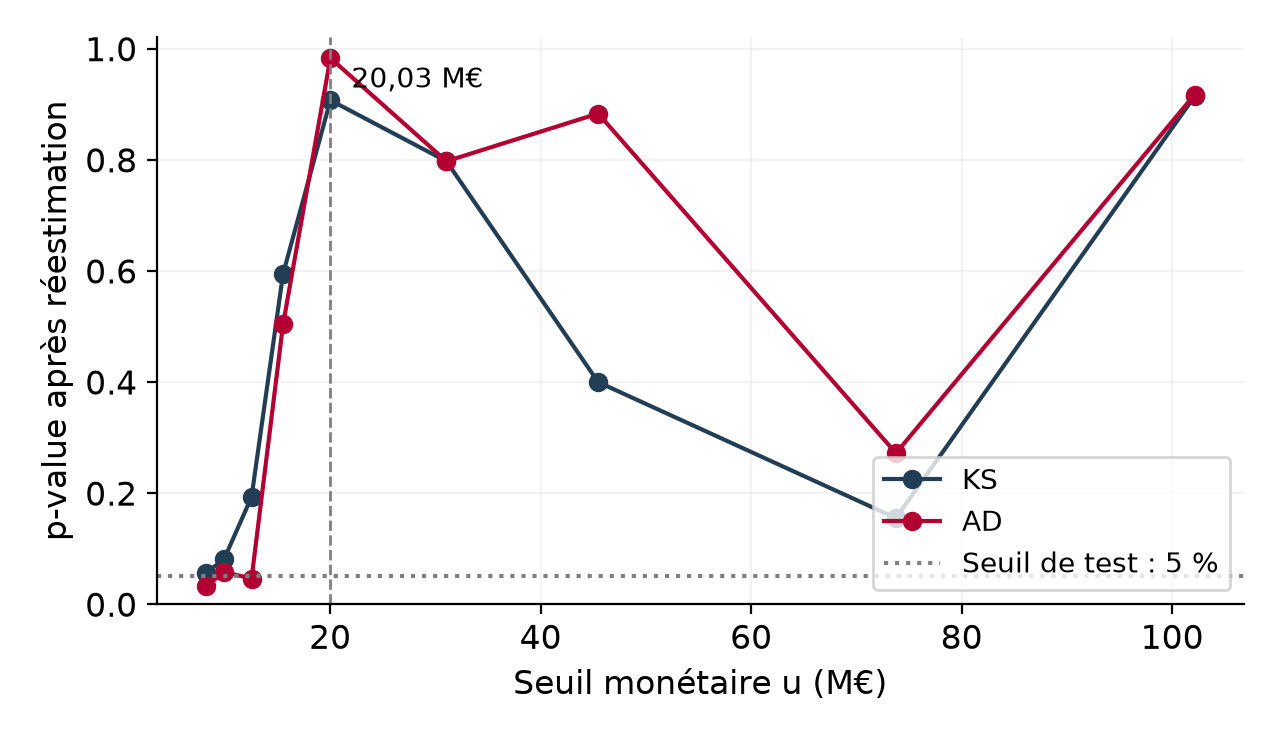
\includegraphics[width=\linewidth]{../../vasicek_lab/figures_inst/G129_tests_seuils.png}
    \column{.43\textwidth}
    \renewcommand{\arraystretch}{1.0}
    % Généré depuis 129.json par outils/ci/actualiser_complements_hugo.py.
\small\textbf{Indice et IC bootstrap à 95 \%}\\[2mm]
\begin{tabular}{@{}lcc@{}}\toprule Estimateur & $\hat\xi$ & IC 95 \% \\\midrule
EMV & 0{,}595 & [0{,}252 ; 0{,}897] \\
PWM & 0{,}505 & [0{,}254 ; 0{,}622] \\
Hill & 1{,}402 & [1{,}208 ; 1{,}605] \\
Moments & 0{,}863 & [0{,}498 ; 1{,}092] \\
\bottomrule\end{tabular}\\[2mm]
\footnotesize Seuil fixé : 20,03 M€.\\
Les intervalles portent sur les excès observés ; ils n’intègrent pas le choix du seuil.

  \end{columns}
  \vspace{0mm}\small Le seuil retenu reste \textbf{20,03 M€} ; les diagnostics évaluent sa compatibilité avec la GPD, sans établir un optimum.\par
  Hill dépasse l'EMV : un écart que la simulation reproduit sous $\xi=0{,}595$ (rapport, chapitre 4).
  \source{script 129, complément après dépôt. KS : Kolmogorov-Smirnov ; AD : Anderson-Darling. EMV : maximum de vraisemblance ; PWM : moments pondérés. IC bootstrap à 95\,\%.}
\end{frame}


% =============================================================================
\section{Cascade et états}
\begin{frame}[t]{Comment relier la conformité au capital ?}
  \framesubtitle{Quatre canaux ; paramètres de conformité posés (chapitres 4 à 6) ; cadres rouges : ajouts}
  \centering
  \resizebox{.99\linewidth}{!}{%
  \begin{tikzpicture}[x=1mm,y=1mm,
    bloc/.style={draw=nexialog!65,fill=white,align=center,inner sep=1mm,
      font=\fontsize{6.5}{7.6}\selectfont},
    canal/.style={fill=nexialog,text=white,rounded corners=.5mm,
      align=center,text width=23mm,inner sep=1mm,font=\fontsize{7}{8.2}\selectfont},
    flux/.style={-{Stealth[length=1.3mm]},draw=nexialog!75,line width=.6pt}]
    \path[use as bounding box] (0,-55) rectangle (146,0);
    % 1 : état latent et deux seuils, comme dans le croquis.
    \node[bloc,draw=accent,line width=.9pt,minimum width=28mm,minimum height=54mm] (etat) at (14,-27) {};
    \node[align=center,font=\fontsize{7}{8.2}\selectfont,text=nexialog] at (14,-5.5)
      {\textbf{1 · État de conformité}\\pour chaque pilier};
    \node[font=\fontsize{7}{8.2}\selectfont] at (14,-12.5)
      {$C^\star=\gamma\Theta+\sqrt{1-\gamma^2}\,\varepsilon$};
    \draw[nexialog!60,->] (2,-19)--(26,-19);
    \foreach \x/\lab in {10/{$K_{\rm bas}$},18/{$K_{\rm haut}$}}{
      \draw[nexialog] (\x,-18)--(\x,-20);
      \node[below,font=\fontsize{5.5}{6}\selectfont] at (\x,-20) {\lab};}
    \foreach \x/\lab in {5/NC,14/PC,23/C}
      \node[font=\fontsize{6}{7}\selectfont,text=nexialog] at (\x,-16.5) {\lab};
    \draw[filet] (3,-26)--(25,-26);
    \node[anchor=north west,align=left,text width=24.5mm,inner sep=0pt,font=\fontsize{5.6}{7}\selectfont,text=gris] at (2,-27.5)
      {NC : non conforme\\PC : partiellement conforme\\C : conforme\\[1mm]
       $C^\star$ : capacité latente\\$\Theta$ : facteur commun\\$\varepsilon$ : choc propre\\$\gamma$ : charge du facteur\\$K$ : seuils de classement};
    \begin{uncoverenv}<2->
    % 2 : quatre canaux, alignés avec leurs trois mécanismes.
    \node[bloc,draw=accent,line width=.9pt,fill=nexialog!5,minimum width=27mm,minimum height=54mm] at (46.5,-27) {};
    \node[font=\fontsize{7}{8.2}\selectfont,text=nexialog] at (46.5,-3) {\textbf{2 · Quatre canaux}};
    \node[canal] (lambda) at (46.5,-9) {Fréquence $\lambda$\\moyenne d'incidents/an};
    \node[canal] (pu) at (46.5,-26) {Détection $p_u$\\probabilité de dépasser $u$};
    \node[canal] (gain) at (46.5,-38.5) {Propagation $g$\\intensité des transmissions};
    \node[canal] (acc) at (46.5,-49.5) {Accumulation\\prestataire commun};
    \draw[flux] (etat.east)--(33,-27);
    % 3--5 : lois et matrice ; T remplace l'ancien nom de code TRANS.
    \node[bloc,text width=40mm,minimum height=17mm] (freq) at (86,-9) {
      \textcolor{nexialog}{\textbf{3 · Fréquence} (ch. 4)}\\[.6mm]
      $N$ : nombre annuel, loi binomiale négative\\[.8mm]
       $\lambda$ : moyenne ; $\varphi=9{,}20$\\[.5mm]
      $\varphi=\mathrm{Var}(N)/\mathbb E[N]$ : dispersion.};
    \node[bloc,text width=40mm,minimum height=17mm] (sev) at (86,-27.5) {
      \textcolor{nexialog}{\textbf{4 · Sévérité} (ch. 4)}\\[.6mm]
      Excès : Pareto généralisée (GPD)\\[.7mm]
      $\xi$ : forme ; $\sigma$ : échelle des pertes\\[.6mm]
      $Y_k=0$ avec prob. $1-p_u$,\\sinon $u+\mathrm{GPD}(\xi,\sigma)$ ; $u=20{,}03$ M€.};
    \node[bloc,draw=accent,line width=.9pt,text width=40mm,minimum height=17mm] (casc) at (86,-46) {
      \textcolor{nexialog}{\textbf{5 · Cascade dirigée} (ch. 5)}\\[.7mm]
      $W=g\,\dfrac{T}{\max_j\sum_k T_{jk}}$\\[.7mm]
      $T$ : forces des liens ; $W$ : probabilités.\\
      $S_a$ : piliers touchés depuis l'amorce $a$.\\
      Si amorce P4 : accumulation.};
    \draw[flux] (lambda.east)--(freq.west);
    \draw[flux] (pu.east)--(sev.west);
    \draw[flux] (gain.east)--([yshift=3mm]casc.west);
    \draw[flux] (acc.east)--([yshift=-3mm]casc.west);
    \end{uncoverenv}
    \begin{uncoverenv}<3->
    % 6--7 : un bloc final commun, rouge Nexialog comme dans la référence.
    \node[bloc,draw=accent,fill=accent,text=white,text width=27mm,minimum height=35mm] (cap) at (131,-27) {
      \textbf{6–7 · Pertes et capital}\\[2mm]
      $X_n=\displaystyle\sum_{k\in S_a}Y_{n,k}$\\[1mm]
      perte d'un sinistre\\[2mm]
      $\VaR_{99{,}5\%}\!\left(\displaystyle\sum_{n=1}^{N}X_n\right)$\\[1mm]
      quantile de la charge\\annuelle agrégée};
    \draw[flux] (freq.east)--node[above,font=\scriptsize] {$N$} ([yshift=11mm]cap.west);
    \draw[flux] (sev.east)--node[above,font=\scriptsize] {$Y_k$} (cap.west);
    \draw[flux] (casc.east)--node[below,font=\scriptsize] {$S_a$} ([yshift=-11mm]cap.west);
    \node[align=center,font=\fontsize{6}{7.2}\selectfont,text=nexialog] (ent) at (131,-51)
      {\textbf{8 · À l'échelle d'une entité}\\$A$ : actifs ; $m(A)$ : facteur de perte};
    \draw[flux] (cap.south)--(ent.north);
    \end{uncoverenv}
  \end{tikzpicture}}
  \source{rapport, chapitres 4 à 6 et 9. États et écarts entre états supposés ; capital de scénario, niveau illustratif.}
\end{frame}

\begin{frame}{Comment l'état évolue-t-il dans le temps ?}
  \suivimethode{1}{État}
  \framesubtitle{\ajout Deux horloges : cascade rapide, conformité lente}
  \begin{columns}[T,onlytextwidth]
    \column{.50\textwidth}\scriptsize
    \setlength{\abovedisplayskip}{.5mm}\setlength{\belowdisplayskip}{.5mm}
    \textbf{Couche rapide.} Les incidents et leur cascade, dans l'année, conditionnellement à une configuration de conformité : un Vasicek multi-états classe chaque pilier non conforme (NC), partiellement conforme (PC) ou conforme (C).
    \setlength{\jot}{0pt}
    \[\begin{aligned}
      \mathbb P(\mathrm{NC}\mid\Theta)&=\Phi\Big(\frac{K_{\mathrm{bas}}-\gamma\Theta}{\sqrt{1-\gamma^2}}\Big),\\
      \mathbb P(\mathrm C\mid\Theta)&=1-\Phi\Big(\frac{K_{\mathrm{haut}}-\gamma\Theta}{\sqrt{1-\gamma^2}}\Big).
    \end{aligned}\]
    Masses d'état posées (0,35, 0,35 et 0,30), ancrées sur les enquêtes de fin 2025 ; en crise,
    davantage de non-conformité. $\gamma=0{,}68$ donne une corrélation de $0{,}462$ entre piliers.\par\vspace{.5mm}
    \textbf{Couche lente.} Une chaîne de Markov NC $\to$ PC $\to$ C, séjours de type phase (Erlang), conforme absorbant dans le cas de base :
    \[\mathrm{SCR}(t)=\sum_{e\in\{\mathrm{NC},\mathrm{PC},\mathrm C\}}\mathbb P(e,t)\,\mathrm{SCR}_e\]
    Moyenne de quantiles, qui diffère du quantile du mélange d'environ $9{,}3\,\%$.
    \column{.46\textwidth}
    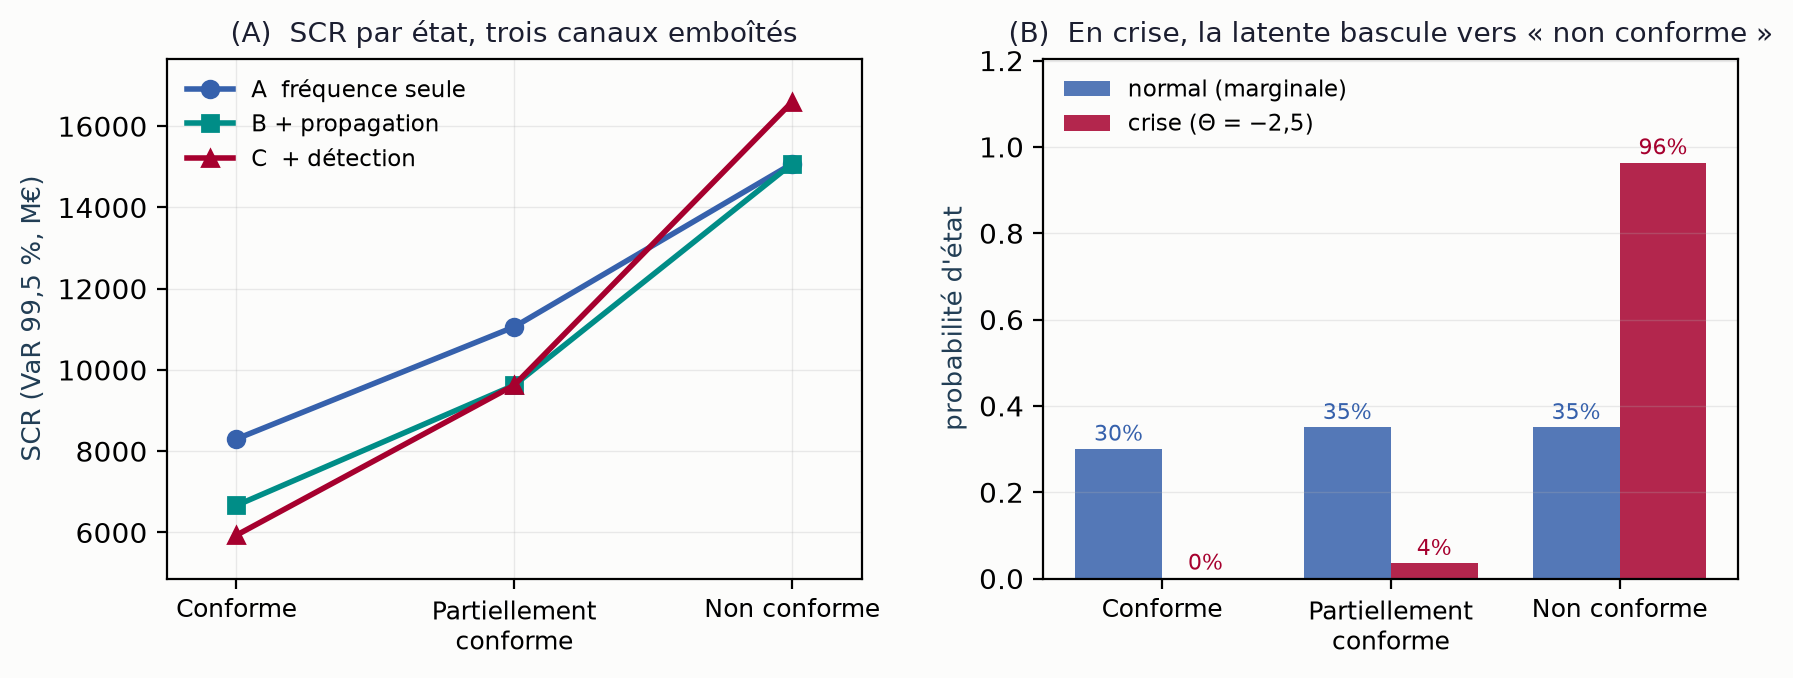
\includegraphics[width=\linewidth]{S10_scr_multi_etats.png}\par
    {\tiny\color{gris}(A) Besoin de capital par état, en cumulant fréquence, propagation puis détection. (B) Probabilités d'état en régime normal et en crise systémique.\par}
    \scriptsize\vspace{.5mm}
    Le même facteur $\Theta$ agit sur les deux couches : un environnement dégradé ralentit la remédiation ($\beta_{\mathrm{rem}}=0{,}35$) et durcit la cascade ($\beta_{\mathrm{casc}}=0{,}1$), deux formes exponentielles posées.
  \end{columns}
  \source{rapport, chapitre 6 (§ 6.1, 6.2, 6.6 et 6.7, figure 6.1). Séparer les horloges évite qu'une tendance longue explique un enchaînement de quelques heures.}
\end{frame}

\begin{frame}{Comment l'état règle-t-il la propagation ?}
  \suivimethode{1,2,5}{État et propagation}
  \framesubtitle{\ajout État de conformité $\longrightarrow$ gain $g$ $\longrightarrow$ matrice $W$}
  \begin{columns}[T,onlytextwidth]
  \column{.48\textwidth}\small
  \textbf{1 · Construire l'état}
  \[C^\star=\gamma\Theta+\sqrt{1-\gamma^2}\,\varepsilon\]
  $\Theta$ : facteur commun ; $\varepsilon$ : choc propre.\par
  Normales centrées réduites indépendantes.\par
  $\gamma=0{,}68$ : charge du facteur commun.\par\vspace{1mm}
  $U=\Phi(C^\star)$ : score uniforme entre 0 et 1.\par\vspace{2mm}
  \begin{tikzpicture}[x=1mm,y=1mm]
  \fill[accent] (0,0) rectangle (19.6,5);
  \fill[acier] (19.6,0) rectangle (39.2,5);
  \fill[nexialog] (39.2,0) rectangle (56,5);
  \foreach \x/\l in {9.8/NC,29.4/PC,47.6/C}
    \node[text=white,font=\small] at (\x,2.5) {\l};
  \foreach \x/\l in {0/0,19.6/{0,35},39.2/{0,70},56/1}
    \node[below,font=\footnotesize] at (\x,0) {\l};
  \end{tikzpicture}
  \column{.47\textwidth}\small
  \textbf{2 · Associer un gain posé}\par\vspace{2mm}
  \renewcommand{\arraystretch}{1.3}
  \begin{tabular}{@{}lccc@{}}\toprule
  État & NC & PC & C \\\midrule
  $g$ & 0,90 & 0,68 & 0,45 \\\bottomrule
  \end{tabular}\par\vspace{1mm}
  \textbf{3 · Normaliser la propagation}
  \[W=g\frac{T}{s_{\max}},\qquad s_{\max}=\max_j\sum_k t_{jk}\]
  $T=(t_{jk})$ : force posée du lien $j\to k$.\par
  $s_{\max}=2{,}6$ : émission maximale.\par
  $W_{jk}$ : probabilité de transmission.
  \end{columns}
  \vspace{1mm}\small Chaque ligne somme à au plus $g<1$ : le rayon spectral vérifie $\rho(W)\le g$.
  \source{rapport, chapitres 5 et 6. NC : non conforme ; PC : partiellement conforme ; C : conforme. $\Phi$ : fonction de répartition normale standard. Seuils sur $C^\star$ : $\Phi^{-1}(0{,}35)$ et $\Phi^{-1}(0{,}70)$.}
\end{frame}

\begin{frame}{D'où vient le multiplicateur de fréquence ?}
  \suivimethode{2,3}{Canaux, fréquence}
  \framesubtitle{\ajout Quatre canaux ; parts Hackmageddon $\times$ effets publiés}
  \begin{columns}[T,onlytextwidth]
    \column{.47\textwidth}\scriptsize
    \renewcommand{\arraystretch}{1.1}
    \begin{tabularx}{\linewidth}{@{}>{\bfseries}l Y r r@{}}
      \toprule
      Canal & Paramètre & C & NC \\
      \midrule
      Fréquence & $\lambda$, incidents par an & 21,56 & 53,62 \\
      \rowcolor{clair}Propagation & $g$, gain de la normalisation & 0,45 & 0,90 \\
      Détection & $p_u$, dépassement par pilier touché & 0,128 & 0,181 \\
      \rowcolor{clair}Accumulation & $\omega$, probabilité de choc commun & 0 & 0,68 \\
      \bottomrule
    \end{tabularx}\par\vspace{1.5mm}
    Statuts : multiplicateur de fréquence posé ; valeurs de $g$ posées ; détection par multiplicateurs $0{,}85$ et $1{,}20$ posés ; accumulation en borne haute posée, non identifiée.\par\vspace{1.2mm}
    $\omega$ est une probabilité de choc et $\gamma$ une charge de facteur : les deux paramètres sont distincts, bien que posés à la même valeur $0{,}68$.\par\vspace{1.2mm}
    Aux bornes des fourchettes, le multiplicateur va de $1{,}933$ à $3{,}042$ : $\lambda_{\mathrm{NC}}$ de $41{,}7$ à $65{,}6$ incidents par an.
    \column{.49\textwidth}\scriptsize
    $\lambda_{\mathrm{NC}}=\lambda_{\mathrm C}\sum_v\pi_v\,m_v$, où $\pi_v$ est la part du vecteur et $m_v$ le centre d'une fourchette de multiplicateur.\par\vspace{1mm}
    \renewcommand{\arraystretch}{1.1}
    \begin{tabularx}{\linewidth}{@{}Y r l r r@{}}
      \toprule
      Vecteur & $\pi_v$ & Fourchette & Centre & $\pi_v m_v$ \\
      \midrule
      Hameçonnage & 0,388 & [1,8 ; 3,0] & 2,40 & 0,9312 \\
      \rowcolor{clair}Exploitation & 0,338 & [2,0 ; 2,6] & 2,30 & 0,7774 \\
      Chaîne d'approv. & 0,158 & [1,9 ; 2,6] & 2,25 & 0,3555 \\
      \rowcolor{clair}Identifiants & 0,063 & [3,0 ; 8,0] & 5,50 & 0,3465 \\
      Autres & 0,053 & [1,3 ; 1,6] & 1,45 & 0,0769 \\
      \midrule
      \multicolumn{4}{@{}l}{\textbf{Multiplicateur agrégé, état non conforme}} & \textbf{2,4875} \\
      \bottomrule
    \end{tabularx}\par\vspace{1mm}
    $21{,}56\times 2{,}4875=53{,}62$ incidents par an. Fourchettes ancrées sur des effets publiés ; « autres » n'a aucune source dédiée. Les identifiants, $6{,}3\,\%$ des incidents, pèsent $13{,}9\,\%$ du multiplicateur. Quatre jeux de parts de 2025--2026 donnent $2{,}318$ à $2{,}471$ : au plus $6{,}8\,\%$ d'écart.
  \end{columns}
  \source{rapport, chapitre 4 (§ 4.3) et chapitre 6 (§ 6.3). Le multiplicateur est posé, non calibré ; l'écart entre états est posé pour les quatre canaux.}
\end{frame}

\begin{frame}{La contagion s'éteint-elle ?}
  \suivimethode{5}{Cascade}
  \framesubtitle{\etabli Normalisation de Leontief et sous-criticité}
  \begin{columns}[T,onlytextwidth]
    \column{.52\textwidth}\scriptsize
    \setlength{\abovedisplayskip}{.5mm}\setlength{\belowdisplayskip}{.5mm}
    \textbf{Le problème.} La matrice d'expert $T$ ne peut servir telle quelle : $\rho(T)=1{,}461>1$ et $(I-T)^{-1}$ compte 21 entrées négatives sur 25 : un choc positif produirait un stress négatif ailleurs.\par\vspace{.8mm}
    \textbf{Le correctif.} Lire la ligne $j$ comme les parts du stress que $j$ émet :
    \[W=g\,\frac{T}{s_{\max}},\quad s_{\max}=\max_j\sum_k t_{jk}=2{,}6,\quad \rho(W)\le g\le 1\]
    Chaque ligne somme à au plus $g$ ; numériquement $\rho(W)=0{,}562\,g$ : sous-critique sur tout le domaine admissible.\par\vspace{.8mm}
    \textbf{Le branchement.} À incidence de fond $4{,}5\,\%$ et $g=0{,}90$ : $\rho(W)=0{,}506$ et $R_0=\rho(M)=0{,}054$. Les seuils critiques, $g=1{,}78$ pour $\rho(W)=1$ et $g=8{,}1$ pour $R_0=1$, sont hors du domaine $g\le 1$.\par\vspace{.8mm}
    \textbf{Progéniture} (incidents causés par un incident) : $0{,}109$ (P1), $0{,}069$ (P4), $0{,}058$ (P2), $0{,}054$ (P3), $0{,}026$ (P5), soit le classement du barème ROOT. Les deux venant du même expert, c'est un test de cohérence interne, non une validation externe.
    \column{.44\textwidth}
    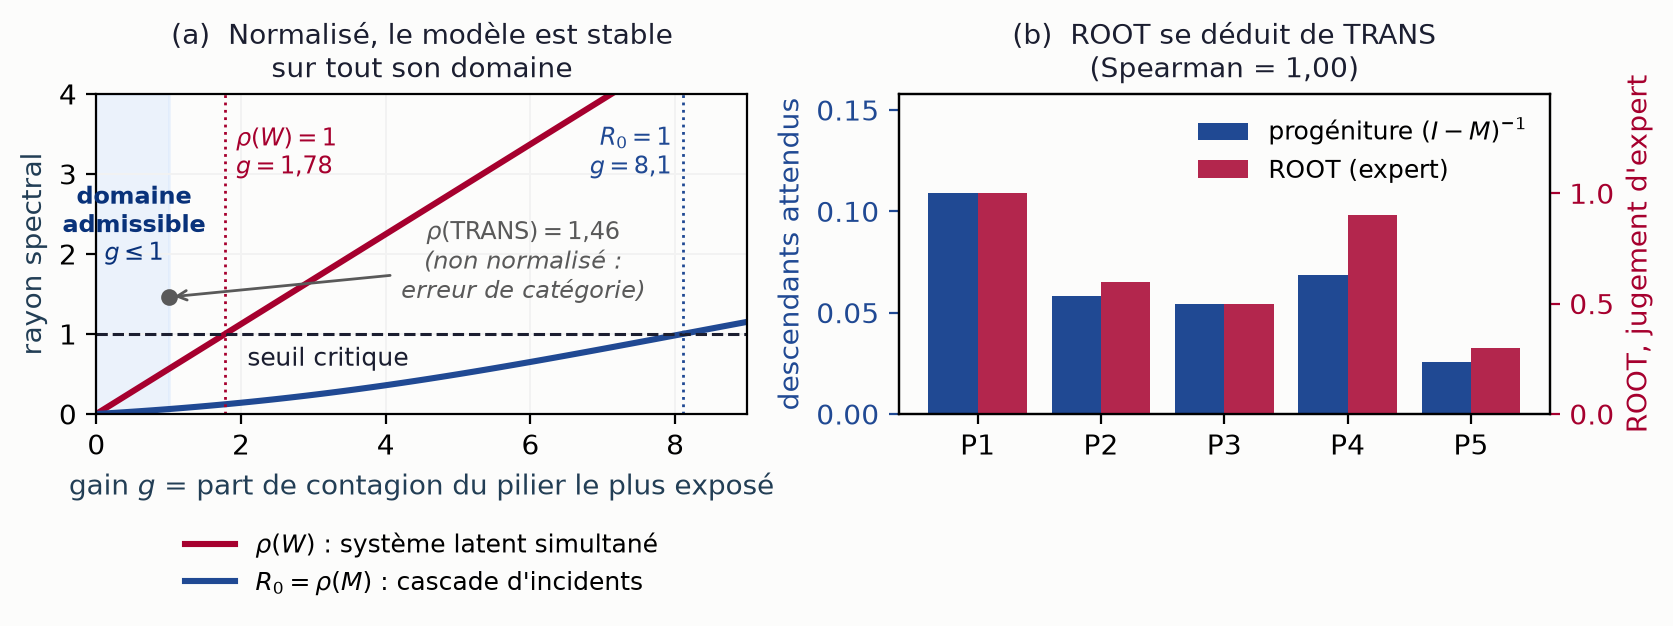
\includegraphics[width=\linewidth]{K3_branchement_R0.png}\par
    {\tiny\color{gris}(a) Rayons spectraux sur le domaine admissible $g\le1$ ; seuils critiques hors domaine. (b) La progéniture reproduit le classement ROOT.\par}
  \end{columns}
  \source{rapport, chapitre 5 (§ 5.4 et 5.5, figure 5.3, proposition 5.3). Nous ne revendiquons pas de non-transitivité : zéro violation sur 420 triplets.}
\end{frame}

\begin{frame}{Peut-on définir un seuil propre à chaque entité ?}
  \suivimethode{5}{Stress et déclenchement}
  \framesubtitle{Le cadre individuel est possible ; les données ne permettent pas sa calibration ici}
  \begin{columns}[T,onlytextwidth]
    \column{.48\textwidth}\footnotesize
    \textbf{Cadre général, pour un stress élevé}\par
    \[K_{ij}=F_{ij}^{-1}(1-p_{ij}),\qquad
      \mathbb P(X_{ij}>K_{ij})=p_{ij}.\]
    $i$ : entité ; $j$ : pilier ; $X_{ij}$ : stress latent ; $F_{ij}$ : sa fonction de répartition,
    supposée continue ; $p_{ij}$ : probabilité cible ; $K_{ij}$ : seuil sans unité monétaire.\par\vspace{2mm}
    Écrire $F_i$ suppose la même marge de stress entre piliers d'une entité.
    Cette propriété n'est pas automatique après propagation.\par\vspace{2mm}
    À probabilités et dépendance inchangées, transformer une marge et son seuil ensemble conserve les déclenchements.
    \column{.48\textwidth}\footnotesize
    \textbf{Méthode retenue}\par\vspace{2mm}
    Les sources étudiées ne permettent pas d'identifier les distributions de stress et les probabilités
    à la maille entité $\times$ pilier.\par\vspace{2mm}
    Le cadre simplifié conserve une loi latente de référence commune :
    \[K_j=F_{\mathrm{latent}}^{-1}(1-p_j).\]
    $p_j$ est alors la probabilité cible du pilier $j$, commune aux entités.\par\vspace{1mm}
    Le moteur de capital simule directement la fréquence, les ensembles de piliers touchés et leurs pertes,
    puis estime le quantile annuel. Il n'utilise pas de $F_{ij}$ estimées.\par\vspace{2mm}
    Le taux $p_u$ de dépassement d'une sévérité élémentaire n'est pas la probabilité annuelle d'incident d'une entité.
  \end{columns}
  \source{rapport, chapitre 5, section sur les seuils ; audits des seuils individuels du 22 octobre.}
\end{frame}

\begin{frame}{Que change l'ordre d'atteinte des piliers ?}
  \suivimethode{5}{Cascade}
  \framesubtitle{\ajout Une dépendance dirigée qu'une copule ne représente pas}
  \begin{columns}[T,onlytextwidth]
    \column{.49\textwidth}\scriptsize
    \setlength{\abovedisplayskip}{.5mm}\setlength{\belowdisplayskip}{.5mm}
    \textbf{Vraisemblance d'une chaîne ordonnée}
    \[\ell(i_1,\dots,i_n)=\mathrm{ROOT}_{i_1}\prod_{k=1}^{n-1}t_{i_ki_{k+1}}\]
    Sur deux piliers, $\ell$ est invariante par permutation si et seulement si $\mathrm{ROOT}_i\,t_{ij}=\mathrm{ROOT}_j\,t_{ji}$. Le barème d'expert viole cette condition pour la paire (P1, P2).\par\vspace{1mm}
    Sur les 26 sous-ensembles d'au moins deux piliers, \textbf{22 changent de criticité} selon l'ordre, de jusqu'à 6 points sur 10. Sur $\{P_1,P_2\}$ : $t_{12}=0{,}80$, $t_{21}=0{,}20$, criticités 8 et 2 pour le même ensemble.\par\vspace{1mm}
    Ni une copule ni un score additif des indicatrices ne représentent cet objet.\par\vspace{1.5mm}
    \textbf{Deux constructions de la cascade.} La cascade indépendante (Bernoulli par arête, percolation) est la seule définie quand une ligne de $W$ somme à plus de un : elle sert aux bornes. La marche auto-évitante, un successeur par pas, sert aux capitaux. Passer de l'une à l'autre déplace le secteur de $-4\,\%$.
    \column{.47\textwidth}\scriptsize
    {\editorial\normalsize Une matrice et sa transposée}\par\vspace{1mm}
    Au premier ordre, la co-occurrence ne dépend de $W$ que par $S=\tfrac12(W+W^\top)$ : $W$ et $W^\top$ y sont indiscernables. La loi complète des ensembles touchés, elle, les distingue.\par\vspace{1mm}
    \renewcommand{\arraystretch}{1.12}
    \begin{tabular}{@{}lrr@{}}
      \toprule
      À $g=0{,}90$ & Sous $W$ & Sous $W^\top$ \\
      \midrule
      Piliers touchés en moyenne & 1,931 & 1,746 \\
      Sinistres multi-piliers & 62,31\,\% & 50,77\,\% \\
      Co-défaillance P2--P5 & 0,127 & 0,066 \\
      \bottomrule
    \end{tabular}\par\vspace{1.2mm}
    Retourner la matrice déplace le capital de $3{,}6\,\%$ (295 M€), la perte moyenne de $7{,}9\,\%$, et le pilier à remédier en premier passe de P1 à P4. Sur l'ensemble admissible, l'écart entre une matrice et sa transposée atteint 1\,173 M€.\par\vspace{1mm}
    {\color{accent}Les statistiques disponibles ne permettent pas cette distinction} : sous amorce uniforme et $W$ divisée par cinquante, l'écart moyen est de $0{,}86\,\%$.
  \end{columns}
  \source{rapport, chapitre 5 (§ 5.8 et 5.9, propositions 5.4 à 5.7). Test de permutation de l'asymétrie sur OpRisk : 119 contre 128 $\pm$ 27, $z=-0{,}33$.}
\end{frame}

\begin{frame}{Combien de piliers un sinistre touche-t-il ?}
  \suivimethode{5,6}{Cascade, perte}
  \framesubtitle{\ajout La défaillance simultanée est la sortie du modèle}
  \begin{columns}[T,onlytextwidth]
    \column{.50\textwidth}\scriptsize
    \renewcommand{\arraystretch}{1.05}
    \begin{tabularx}{\linewidth}{@{}Y r r@{}}
      \toprule
      & Conforme & Non conforme \\
      \midrule
      Sinistres multi-piliers, cascade seule & 31,15\,\% & 62,31\,\% \\
      \rowcolor{clair}\quad avec le choc commun P4 & --- & 73,25\,\% \\
      Piliers touchés en moyenne, cascade seule & 1,38 & 1,93 \\
      \rowcolor{clair}\quad avec le choc commun P4 & --- & 2,44 \\
      Quantile 99,5\,\% / celui d'un incident & 1,27 & 1,58 \\
      \bottomrule
    \end{tabularx}\par\vspace{1.5mm}
    La loi du nombre de piliers touchés est exacte (énumération). À l'état non conforme, la défaillance simultanée est majoritaire. Avec le choc commun P4, le rapport au quantile d'un incident vaut $1{,}85$ : ce n'est pas un effet sur le capital annuel, le double comptage est chiffré, non corrigé.
    \column{.46\textwidth}\scriptsize
    {\editorial\normalsize « Additif » désigne trois choses}\par\vspace{1mm}
    \textbf{(i) Au sein d'un sinistre.} Les coûts des piliers touchés s'additionnent : \textcolor{accent}{hypothèse de construction, non testée}. Chaque pilier tire sa perte dans la loi calibrée sur des incidents complets.\par\vspace{1mm}
    \textbf{(ii) En fonction des piliers non conformes.} Le capital est presque additif : $R^2=0{,}9945$ sur les 32 configurations (6\,015 à 17\,009 M€), contributions de 3\,524 (P1), 2\,863 (P4), 2\,022 (P2), 1\,577 (P3) et 897 M€ (P5). \textcolor{accent}{Mesure.}\par\vspace{1mm}
    \textbf{(iii) En fonction des quatre canaux.} Le capital est super-additif : $+5\,001$ M€ d'interaction sur 14\,139, soit $+35\,\%$. \textcolor{accent}{Mesure.}\par\vspace{1.5mm}
    Répondre « le modèle est super-additif » est faux : il l'est sur les canaux, pas sur les piliers, et l'hypothèse sur les coûts est un troisième objet.
  \end{columns}
  \source{rapport, chapitre 6 (§ 6.5.1), chapitre 9 (§ 9.1) et chapitre 10 (§ 10.8).}
\end{frame}

\begin{frame}{Le résultat dépend-il des valeurs posées de g ?}
  \suivimethode{2,5}{Canaux, cascade}
  \framesubtitle{\ajout Cinq correspondances état $\to g$, entité notionnelle}
  \begin{columns}[T,onlytextwidth]
    \column{.56\textwidth}\scriptsize
    \renewcommand{\arraystretch}{1.12}
    \begin{tabularx}{\linewidth}{@{}Y r r r r c@{}}
      \toprule
      Application état $\to g$ & C & PC & NC & Écart & Ordre \\
      & M€ & M€ & M€ & & \\
      \midrule
      étroite (0,70 / 0,80 / 0,90) & 145,5 & 156,5 & 169,0 & +16,2\,\% & oui \\
      \rowcolor{clair}\textbf{retenue (0,45 / 0,68 / 0,90)} & 116,4 & 143,2 & 169,0 & +45,2\,\% & oui \\
      large (0,20 / 0,55 / 0,90) & 94,4 & 126,4 & 169,0 & +79,1\,\% & oui \\
      \rowcolor{clair}conformité faible (0,45 / 0,55 / 0,65) & 116,4 & 126,4 & 139,2 & +19,5\,\% & oui \\
      très étroite (0,85 / 0,875 / 0,90) & 162,6 & 166,7 & 169,0 & +3,9\,\% & oui \\
      \midrule
      repère forfaitaire de Formule Standard & 450 & 450 & 450 & 0\,\% & plat \\
      \bottomrule
    \end{tabularx}\par\vspace{1.5mm}
    Le signe et l'ordre de l'écart valent pour toute correspondance qui respecte $g_{\mathrm C}<g_{\mathrm{PC}}<g_{\mathrm{NC}}$ ; seule l'amplitude est un scénario. Même un déplacement de $0{,}05$ sur $g$ donne $+3{,}9\,\%$, quand le forfait reste plat.
    \column{.40\textwidth}\scriptsize
    {\editorial\normalsize Ce qui est vérifié}\par\vspace{1mm}
    Sur une grille de vingt points, à nombres aléatoires communs, aucun pas n'est décroissant, ni pour le capital ni pour la perte moyenne, à l'échelle d'entité comme du secteur. La grille ne démontre pas la propriété pour toute valeur de $g$.\par\vspace{1.2mm}
    L'élasticité d'arc du capital au gain est de $0{,}41$ sur $g\in[0{,}20\,;0{,}95]$ ; un écart de $10\,\%$ ne demande qu'une baisse de $g$ de $0{,}90$ à $0{,}75$.\par\vspace{1.2mm}
    {\color{accent}Hypothèse qui demeure :} qualitative, $g_{\mathrm C}<g_{\mathrm{NC}}$ : se conformer à DORA réduit la propagation entre piliers.
  \end{columns}
  \source{rapport, chapitre 6 (§ 6.4, figure 9.3). Entité notionnelle de 15\,000 M€ de provisions, lecture du registre ; le 169 M€ est une extrapolation d'ordre de grandeur.}
\end{frame}


% =============================================================================
\section{Identifiabilité}
\begin{frame}{Peut-on identifier le sens de la propagation ?}
  \suivimethode{}{}
  \framesubtitle{\ajout $S$ conserve la force commune ; $A$ porte l'asymétrie entre les deux sens}
  \noindent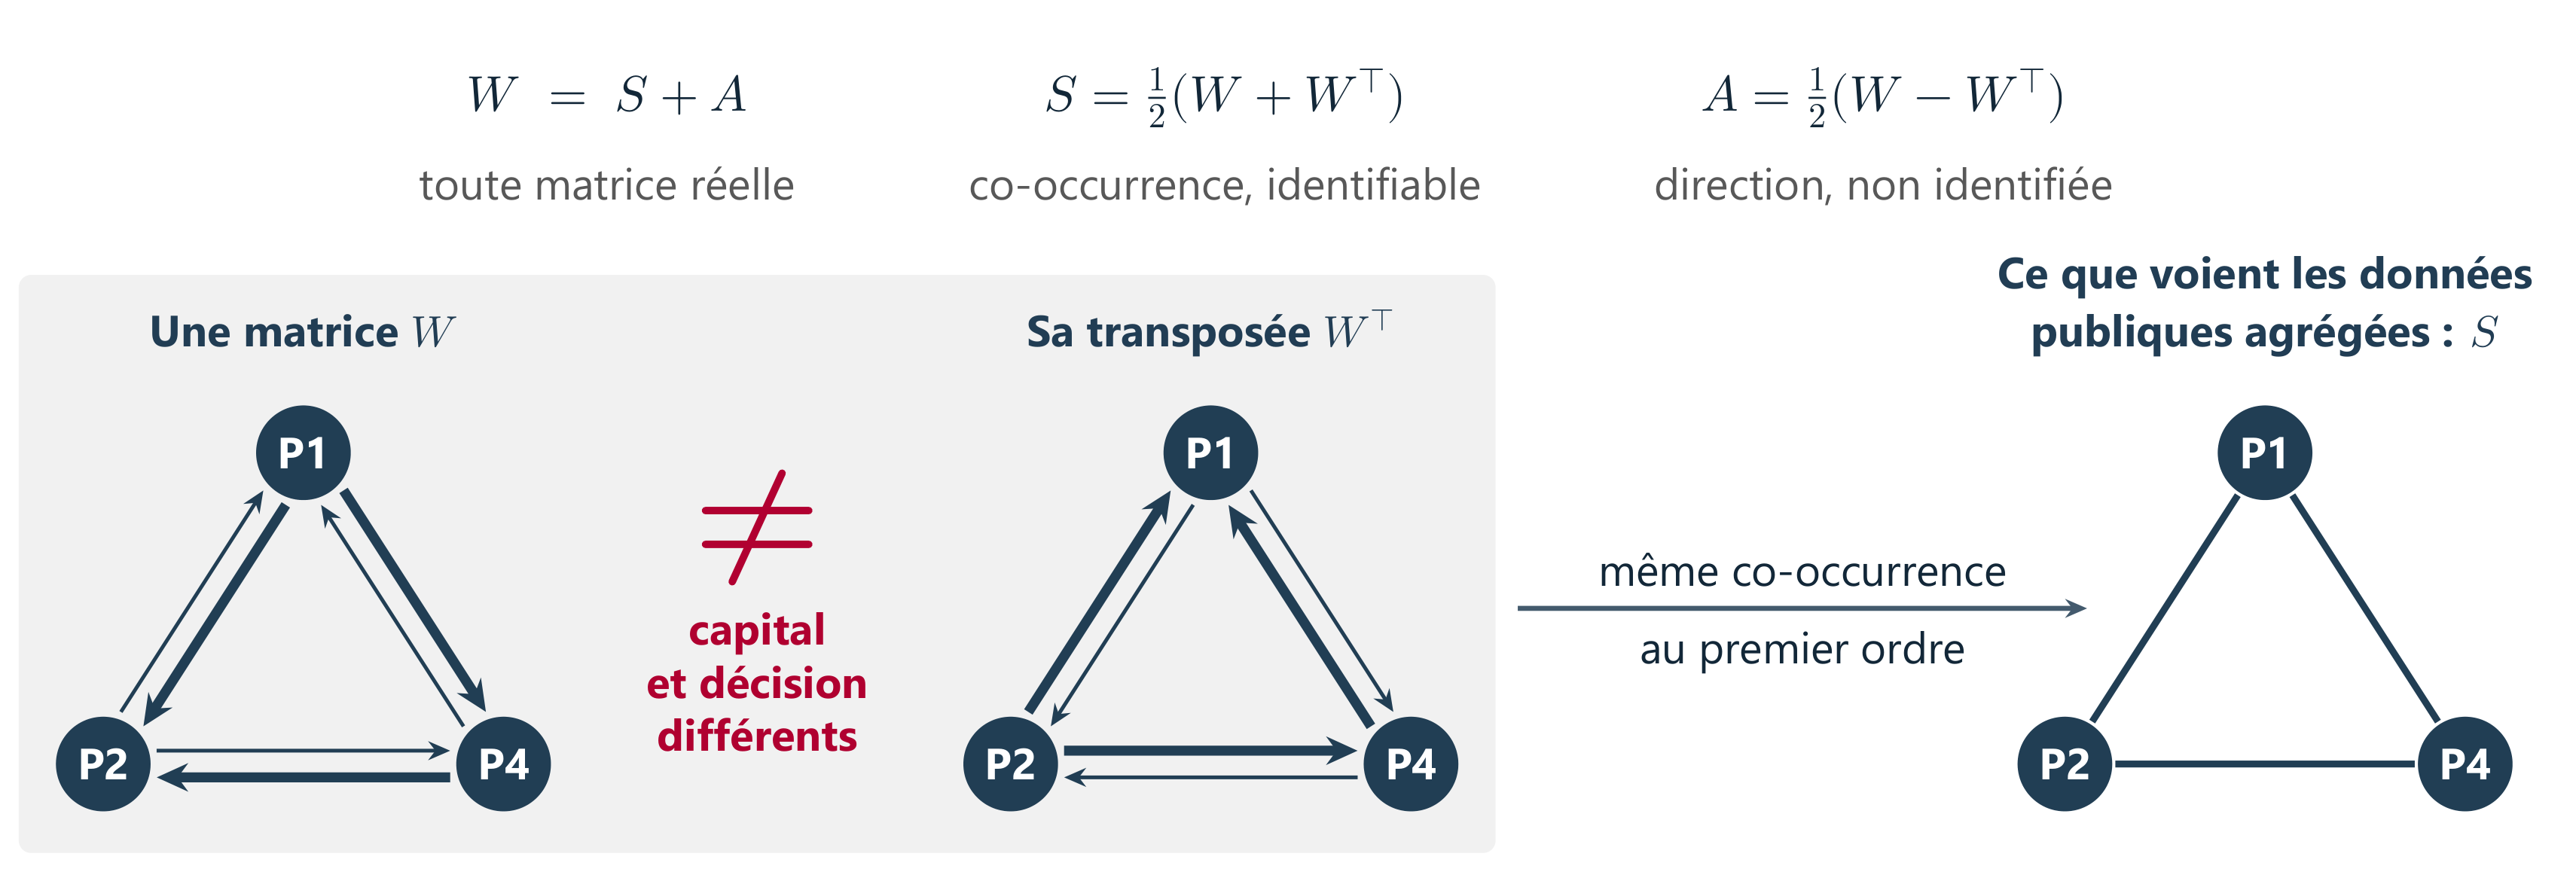
\includegraphics[width=.75\textwidth]{schema_identifiabilite.png}\par\vspace{1mm}
  \small On pose $S$ et l'on fait varier $A$ : les co-occurrences disponibles ne suffisent pas à fixer la direction.
  \only<1>{\question{Si la direction n'est pas identifiable, que peut-on encore dire du capital ?}}
  \uncover<2->{
  \[W^2=S^2+SA+AS+A^2\]
  \small $A$ intervient dès le second ordre : les transmissions en deux pas dépendent de la direction.
  }
  \source{rapport, chapitres 7 et 8. Lecture de la co-occurrence au premier ordre : amorce uniforme, faible intensité. $S$ est posé à dire d'expert dans l'application.}
\end{frame}

\begin{frame}{Que donnent les trois sources agrégées ?}
  \suivimethode{}{}
  \framesubtitle{\ajout Trois sources, trois échecs de nature différente}
  \begin{columns}[T,onlytextwidth]
    \column{.315\textwidth}\scriptsize
    {\editorial\normalsize Chronologie américaine}\par\vspace{.5mm}
    {\color{accent}\textbf{Pas de taxonomie}}\par\vspace{1mm}
    74\,783 incidents, 25\,009 organisations.\par\vspace{.8mm}
    La catégorie non déterminée (\texttt{UNKN}) pèse $52{,}7\,\%$ des incidents ; la date de survenance n'est exploitable que dans $49{,}6\,\%$ des cas, de façon non aléatoire.\par\vspace{.8mm}
    Ordonner par date de déclaration mesurerait le délai de détection, pas la contagion. Restreinte aux types informatifs et aux trimestres consécutifs, la base ne donne que \textbf{71 transitions} ($3{,}6$ par cellule hors diagonale ; 34 en finance).
    \column{.315\textwidth}\scriptsize
    {\editorial\normalsize SAS OpRisk}\par\vspace{.5mm}
    {\color{accent}\textbf{Pas de pas de temps}}\par\vspace{1mm}
    4\,329 transitions annuelles entre 7 catégories de risque, environ 103 par cellule : trop grossier pour saisir une antériorité.\par\vspace{.8mm}
    Placebo par permutation des années à l'intérieur de chaque firme : asymétrie observée $\tau(M)=119$ contre $128\pm 27$, soit $z=-0{,}33$ ; aucune des 18 paires suffisamment peuplées n'est significative à 5\,\%, avant ou après Bonferroni.\par\vspace{.8mm}
    Le test du temps inversé est dégénéré sur un comptage (la matrice renversée est $M^\top$).
    \column{.315\textwidth}\scriptsize
    {\editorial\normalsize VERIS Community}\par\vspace{.5mm}
    {\color{accent}\textbf{Les champs existent, vides}}\par\vspace{1mm}
    10\,591 incidents, dont 980 en secteur financier.\par\vspace{.8mm}
    Domaine de contrôle défaillant (\texttt{control\_failure}) renseigné dans \textbf{13} incidents ($0{,}12\,\%$), dont un seul en finance ; chronologie en quatre étapes datée sur au moins deux étapes dans \textbf{126} ($1{,}19\,\%$), sur au moins trois dans 10.\par\vspace{.8mm}
    L'intersection des deux conditions compte \textbf{1 incident}, hors secteur financier. La spécification existe mais n'est pas remplie.
  \end{columns}
  \vspace{2mm}
  {\color{filet}\rule{\linewidth}{.35pt}}\par\vspace{1.5mm}
  \footnotesize\textbf{Conditions d'identification.} Observer des co-occurrences de défaillances de piliers dans une même entité ; distinguer $W_{jk}$ de $W_{kj}$ (antériorité fiable ou loi complète des ensembles touchés) ; disposer d'une taxonomie par domaine de contrôle. Aucune source ne les réunit.
  \source{rapport, chapitre 7 (§ 7.1 et 7.2).}
\end{frame}

\begin{frame}{La co-occurrence voit-elle le sens ?}
  \suivimethode{5}{Cascade}
  \framesubtitle{\ajout Réversibilité : l'énergie de fluctuation est aveugle à $A$}
  \begin{columns}[T,onlytextwidth]
    \column{.55\textwidth}\scriptsize
    \setlength{\abovedisplayskip}{.5mm}\setlength{\belowdisplayskip}{.5mm}
    \textbf{Décomposition.} $W=S+A$, avec $S=\tfrac12(W+W^\top)$ et $A=\tfrac12(W-W^\top)$, orthogonales au sens de Frobenius. Une co-occurrence est symétrique : elle ne voit que $S$.
    \[\sum_{a}r\,\mathbb P\big(\{j,k\}\subseteq S_a\big)=2r\,S_{jk}+O(\|W\|^2)\]
    \textbf{Chaîne auxiliaire.} De noyau $P$ et de loi stationnaire $\pi>0$, le noyau adjoint est $\tilde P_{jk}=\pi_kP_{kj}/\pi_j$ ; avec $A_\pi=(P-\tilde P)/2$, le courant vaut $J_{jk}=2\pi_j(A_\pi)_{jk}$, nul à l'équilibre détaillé. La forme de Dirichlet
    \[\mathcal E(f,f)=\tfrac12\sum_{j,k}\pi_j(S_\pi)_{jk}\,(f_k-f_j)^2\]
    ne dépend que de la partie réversible : elle est \textbf{aveugle à la direction}. L'invariance par renversement du temps n'interdit pas de détecter l'\emph{intensité} d'une irréversibilité, mais elle ne donne pas le signe du courant.\par\vspace{1mm}
    {\color{accent}Deux limites :} $W$ n'est pas un générateur de Markov au sens strict, et l'énoncé ne s'étend pas à la loi complète des ensembles touchés, qui dépend de $A$.    \column{.41\textwidth}
    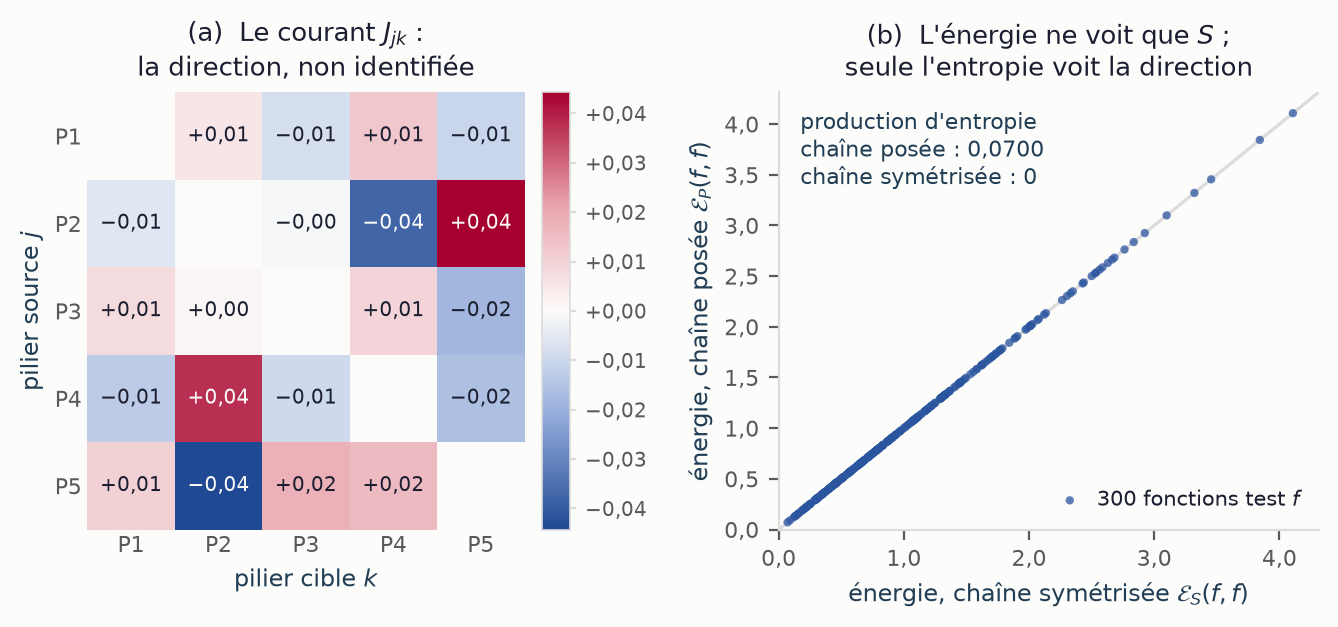
\includegraphics[width=\linewidth]{Z11_reversibilite_martingale.png}\par
    {\tiny\color{gris}(a) Le courant $J_{jk}$ est non nul : le modèle a une direction. (b) Pour trois cents fonctions test, l'énergie de fluctuation est la même pour la chaîne posée et pour sa symétrisée.\par}
  \end{columns}
  \source{rapport, chapitre 5 (proposition 5.7) et chapitre 7 (§ 7.3, figure 7.1). Mesure physique : aucun prix, aucun test de martingalité au sens des générateurs de scénarios.}
\end{frame}

\begin{frame}{Le choc MOVEit révèle-t-il une direction ?}
  \suivimethode{}{}
  \framesubtitle{\ajout Expérience naturelle : un choc exogène, daté, rattaché au pilier P4}
  \begin{columns}[T,onlytextwidth]
    \column{.46\textwidth}\footnotesize
    En mai 2023, l'exploitation de masse d'une faille du logiciel de transfert MOVEit frappe en même temps des centaines d'organisations. Si la contagion dirigée existe, ce choc doit élever, dans les mois suivants, le risque de défaillances relevant d'autres piliers chez les organisations touchées.\par\vspace{2mm}
    \textbf{Différence de différences.} 188 organisations financières touchées, contre un groupe de contrôle apparié, sur des fenêtres de 180 jours : \textbf{+1,17 jour} de déclaration d'incident par organisation (IC bootstrap $[+1{,}07\,;+1{,}27]$).\par\vspace{2mm}
    {\color{accent}Placebo.} Calé sur une fausse date un an plus tôt, le même dispositif donne $+1{,}11$ : l'effet est compatible avec une régression vers la moyenne du groupe de contrôle sélectionné.
    \column{.50\textwidth}
    \centering
    \resizebox{\linewidth}{!}{\begin{tikzpicture}[x=1mm,y=1mm]
      \draw[filet] (0,0)--(78,0);
      \fill[accent] (6,0) rectangle (22,30);
      \fill[acier] (30,0) rectangle (46,28.5);
      \fill[nexialog] (54,0) rectangle (70,1.5);
      \node[above,font=\small\bfseries,text=accent] at (14,30) {$+1{,}17$};
      \node[above,font=\small\bfseries,text=acier] at (38,28.5) {$+1{,}11$};
      \node[above,font=\small\bfseries,text=nexialog] at (62,1.5) {$+0{,}06$};
      \node[below,align=center,font=\scriptsize] at (14,0) {Date réelle\\(mai 2023)};
      \node[below,align=center,font=\scriptsize] at (38,0) {Fausse date\\(un an plus tôt)};
      \node[below,align=center,font=\scriptsize] at (62,0) {Effet net};
    \end{tikzpicture}}\par\vspace{1mm}
    {\scriptsize Jours de déclaration en plus, par organisation touchée.\par}\vspace{2mm}
    \footnotesize\raggedright L'effet net de $+0{,}06$ jour est indiscernable de zéro. La cible resterait de toute façon non attribuable : la source classe les incidents par vecteur d'attaque, avec 32\,\% de non déterminés.
  \end{columns}
  \source{rapport, chapitre 7 (§ 7.4). Résultat négatif publié comme tel ; le choc MOVEit n'identifie ni direction ni amplitude.}
\end{frame}

\begin{frame}{Les rapports suggèrent-ils un ordre ?}
  \suivimethode{5}{Cascade}
  \framesubtitle{\ajout Sept puis dix rapports officiels codés en transitions dirigées}
  \begin{columns}[T,onlytextwidth]
    \column{.56\textwidth}\scriptsize
    \renewcommand{\arraystretch}{1.12}
    \begin{tabularx}{\linewidth}{@{}Y r r r r@{}}
      \toprule
      Périmètre & Rapports & Transitions & Asym. / nul & $z$ \\
      \midrule
      \textbf{Corpus initial} & 7 & 17 & $17\ /\ 8{,}4\pm2{,}2$ & $+3{,}93$ \\
      \rowcolor{clair}Corpus étendu & 10 & 22 & $22\ /\ 9{,}5\pm2{,}4$ & $+5{,}12$ \\
      Sources primaires seules & 7 & 18 & $18\ /\ 8{,}2\pm2{,}4$ & $+4{,}08$ \\
      \rowcolor{clair}Perspective entité seule & 6 & 16 & $16\ /\ 8{,}0\pm2{,}2$ & $+3{,}62$ \\
      \bottomrule
    \end{tabularx}\par\vspace{1.5mm}
    Unité de codage : le couple (incident, paire de piliers). Toutes les transitions vont dans le sens dominant de leur paire ($p=0{,}0004$ sur le corpus initial), là où le pas annuel d'OpRisk donnait $z=-0{,}33$.\par\vspace{1mm}
    \textbf{P1} n'est jamais une cible (9 sorties, 0 entrée) ; \textbf{P2} n'a aucune sortie (0 sortie, 7 entrées) : la structure que le classeur d'expert posait par jugement.
    \column{.40\textwidth}\scriptsize
    {\editorial\normalsize Postérieur bêta par lien}\par\vspace{1mm}
    $p_{jk}\mid\text{données}\sim\mathrm{Beta}(1+m_{jk},\,1+N_j-m_{jk})$ : $N_j$ incidents où $j$ a cédé, $m_{jk}$ où le rapport documente $j\to k$.\par\vspace{1mm}
    Sur les vingt liens, douze ont un intervalle de crédibilité à 90\,\% sous $0{,}5$, aucun au-dessus. Les plus élevés, P3$\to$P2 ($0{,}77$, $[0{,}48\,;0{,}95]$) et P1$\to$P4 ($0{,}68$, $[0{,}40\,;0{,}89]$), recouvrent encore $0{,}5$.\par\vspace{1mm}
    Corrélation avec le classeur d'expert : $\rho=+0{,}08$ sur la matrice, $+0{,}31$ sur sa partie antisymétrique ($p=0{,}19$) : non significative.\par\vspace{1mm}
    {\color{accent}Le placebo teste la cohérence du codage, pas l'exogénéité de la direction} : codeur unique, sources en partie secondaires, échantillon d'incidents notoires.
  \end{columns}
  \source{rapport, chapitre 7 (§ 7.5 et 7.6). Le corpus corrobore la structure sans la calibrer ; fiabilité par second codeur en aveugle en attente.}
\end{frame}

\begin{frame}{Le biais de narration peut-il tout expliquer ?}
  \suivimethode{5}{Cascade}
  \framesubtitle{\ajout Onze des vingt-deux transitions partent de P1}
  \begin{columns}[T,onlytextwidth]
    \column{.50\textwidth}\scriptsize
    Une enquête mandatée pour établir une cause racine conclut souvent à une défaillance de gouvernance : P1 peut ressortir comme source par convention d'écriture. Nous chiffrons ce biais par une loi nulle exacte (convolution) et une borne adverse sur les $2^{11}$ sous-ensembles d'arêtes partant de P1.\par\vspace{1.5mm}
    \renewcommand{\arraystretch}{1.12}
    \begin{tabularx}{\linewidth}{@{}Y r r@{}}
      \toprule
      Hypothèse sur les 11 arêtes de P1 & Reste & $p$ exacte \\
      \midrule
      Aucune (corpus tel que codé) & 22 & $1{,}5\cdot10^{-5}$ \\
      \rowcolor{clair}4 arêtes retournées, pire configuration & 22 & $0{,}084$ \\
      Les 11 arêtes retirées & 11 & $0{,}0039$ \\
      \rowcolor{clair}Les 7 rapports concernés retirés & 3 & $0{,}50$ \\
      \bottomrule
    \end{tabularx}\par\vspace{1.5mm}
    Il faudrait que la convention ait inversé quatre des onze arêtes, dans l'agencement le plus défavorable, pour perdre la significativité. Retirer tout le rôle de la gouvernance ne suffit pas : la direction subsiste dans les chaînes P3$\to$P2 et P4$\to$P2.
    \column{.46\textwidth}\scriptsize
    {\editorial\normalsize Ce que cela coûte en capital}\par\vspace{1mm}
    On dégrade l'émission de P1 par $W_{1k}\to(1-a)\,W_{1k}$ et l'on recalcule la bande à chaque degré.\par\vspace{1.5mm}
    \renewcommand{\arraystretch}{1.12}
    \begin{tabular}{@{}lr@{}}
      \toprule
      Entité notionnelle, M€ & \\
      \midrule
      Besoin à $a=0$ & 169,0 \\
      Besoin à $a=1$ (P1 muette) & 127,1 \\
      Déplacement & 41,9 ($-24{,}8\,\%$) \\
      Largeur de la bande d'identification & 51,7 \\
      \bottomrule
    \end{tabular}\par\vspace{1.5mm}
    Admettre l'objection dans toute son ampleur déplace le niveau de $0{,}81$ fois la largeur de la bande : moins que l'ignorance directionnelle déjà publiée.\par\vspace{1mm}
    Le pilier à remédier en premier passe de P1 à P4 dès $a=0{,}50$ ; l'écart entre états descend de $+45{,}2\,\%$ à $+29{,}1\,\%$ à $a=1$ sans s'annuler, car la conformité agit par $g$ sur toutes les arêtes.
  \end{columns}
  \source{rapport, chapitre 7 (§ 7.7) et chapitre 9 (§ 9.6). Le 169,0 M€ est une extrapolation d'ordre de grandeur, en lecture du registre.}
\end{frame}

\begin{frame}{Que la donnée établit-elle, et que ne fixe-t-elle pas ?}
  \suivimethode{}{}
  \framesubtitle{\ajout La frontière d'identification, en trois niveaux}
  \scriptsize
  \renewcommand{\arraystretch}{1.18}
  \begin{tabularx}{\linewidth}{@{}>{\bfseries}l Y Y@{}}
    \toprule
    Objet & Ce que la donnée établit & Posture retenue \\
    \midrule
    Structure (P1 amont, P2 aval) & 17 transitions sur le corpus initial, 22 sur le corpus étendu, aucune à contre-sens ; $z=+3{,}9$ puis $+5{,}1$ ; accord de la structure avec le classeur d'expert, non des coefficients ($\rho=+0{,}08$) ; codeur unique & \textbf{Revendiquée}, avec son confondant déclaré \\
    \rowcolor{clair}Direction, paire par paire & 2 paires sur 6 seulement ont un intervalle de crédibilité concluant & \textbf{Non revendiquée} ; les bornes restent \\
    Amplitude des coefficients & Aucune information ; même avec les dix sens connus, une bande de 656 M€ subsisterait & \textbf{Non identifiable} par cette voie \\
    \bottomrule
  \end{tabularx}
  \vspace{2mm}
  \begin{columns}[T,onlytextwidth]
    \column{.48\textwidth}\footnotesize
    {\editorial\normalsize Formalisation bayésienne}\par\vspace{1mm}
    Pour chaque paire $\{lo,hi\}$ : $A_{lo,hi}=S_{lo,hi}(2\theta-1)$, avec $\theta\sim\mathrm{Beta}(\alpha_0,\beta_0)$ la probabilité qu'une chaîne documentée aille de $lo$ vers $hi$ ; après $n_{lo}$ et $n_{hi}$ chaînes, $\theta\mid\text{données}\sim\mathrm{Beta}(\alpha_0+n_{lo},\beta_0+n_{hi})$.
    \column{.48\textwidth}\footnotesize
    {\editorial\normalsize Ce que cela donne}\par\vspace{1mm}
    Les quatre paires non documentées gardent un $\theta$ uniforme : le postérieur reproduit l'identification partielle sans la poser. L'intervalle de crédibilité à 90\,\% du capital est $81\,\%$ plus resserré que les bornes de pire cas. Nous retenons les bornes et publions cet intervalle à titre informatif.
  \end{columns}
  \vspace{1.5mm}
  {\color{accent}\footnotesize Nous revendiquons donc un ordre partiel entre piliers ; ce que la donnée ne fixe pas se lit en bande.}
  \source{rapport, chapitre 7 (§ 7.8 et 7.9).}
\end{frame}


% =============================================================================
\section{Identification partielle}
\begin{frame}{1 · Quelles directions faut-il envisager ?}
  \suivimethode{5}{Matrices candidates}
  \framesubtitle{\ajout Un choix de direction pour chaque paire de piliers}
  \vspace{2mm}
  \begin{columns}[T,onlytextwidth]
  \column{.34\textwidth}\centering
  \begin{tikzpicture}[scale=0.95]
    \foreach \n/\a in {1/90,2/18,3/-54,4/-126,5/162}
      \node[pilier] (P\n) at (\a:1.5) {P\n};
    \foreach \i/\j in {1/2,1/3,1/4,1/5,2/3,2/4,2/5,3/4,3/5,4/5}
      \draw[acier] (P\i)--(P\j);
    \draw[fla] (P1)--(P2);
    \node[font=\scriptsize,text=accent,align=center] at (0,-2.35) {chaque arête : un sens à choisir};
  \end{tikzpicture}
  \column{.62\textwidth}\small
  \textbf{Compter.}
  \[\underbrace{\frac{5\times4}{2}=10}_{\text{paires}}\quad\longrightarrow\quad
  \textcolor{accent}{\underbrace{2^{10}=1\,024}_{\text{configurations de signes}}}\]
  \textbf{Construire.} $A_{jk}=\varepsilon_{jk}\,t\,S_{jk}$, avec $\varepsilon_{jk}\in\{-1,+1\}$ et $A_{kj}=-A_{jk}$.\par
  $t$ : amplitude d'asymétrie ; $S$ reste fixé.\par\vspace{2mm}
  \textbf{Filtrer.} Garder $W=S+A$ tel que
  \[0\le W_{jk}\le1,\qquad\rho(W)<1.\]
  {\footnotesize\color{gris}Ces configurations diffèrent des $5!=120$ ordres des cinq piliers.}
  \end{columns}
  \source{rapport, chapitre 8. Sommets d'un pavé, puis filtre d'admissibilité ; les extrema globaux ne sont pas démontrés.}
\end{frame}

\begin{frame}{2 · Que coûte un incident qui se propage ?}
  \suivimethode{4,5,6}{Perte par incident}
  \framesubtitle{Une amorce, des transmissions indépendantes, une sévérité par pilier touché}
  \begin{center}
  \begin{tikzpicture}[node distance=4mm]
    \node[etape] (e1) {\textbf{1. Amorce}\\ Pilier tiré selon les poids de fréquence};
    \node[etape, right=of e1] (e2) {\textbf{2. Transmissions}\\ Chaque arête $j\to k$ avec probabilité $W_{jk}$};
    \node[etape, right=of e2] (e3) {\textbf{3. Ensemble atteint}\\ $S_a$ : piliers touchés, comptés une fois};
    \node[etape, right=of e3] (e4) {\textbf{4. Perte}\\ $X=\sum_{k\in S_a} Y_k$};
    \draw[fl] (e1) -- (e2); \draw[fl] (e2) -- (e3); \draw[fl] (e3) -- (e4);
  \end{tikzpicture}
  \end{center}
  
  \begin{center}
    \centering
    \begin{tikzpicture}[xscale=1.55,yscale=0.85]
      \node[pilier touche] (P1) at (0,1.5) {P1};
      \node[pilier touche] (P2) at (2.0,1.5) {P2};
      \node[pilier] (P3) at (3.8,1.5) {P3};
      \node[pilier touche, fill=accent, draw=accent] (P4) at (1.0,0) {P4};
      \node[pilier] (P5) at (2.9,0) {P5};
      \draw[fla] (P4) -- (P1); \draw[fla] (P4) -- (P2);
      \draw[flnon] (P2) -- (P3); \draw[flnon] (P4) -- (P5);
      \node[font=\scriptsize, text=accent, below=0.5mm of P4] {Amorce};
    \end{tikzpicture}\\[0.5mm]
    {\scriptsize Rouge : transmission réalisée. Pointillés : transmission non réalisée.}
  \end{center}
  \vspace{-0.5mm}
  {\footnotesize Les bornes utilisent cette cascade indépendante, seule définie quand une ligne de $W$ somme à plus de un ; les capitaux par état utilisent la marche auto-évitante. Passer de l'une à l'autre déplace le besoin du secteur de $-4\,\%$ ; bornes et capitaux par état ne se comparent donc pas directement.\par}
  \source{rapport, chapitres 4, 5 et 8.}
\end{frame}

\begin{frame}{3 · Que vaut le capital aux 1\,024 sommets ?}
  \suivimethode{7}{Capital aux sommets}
  \framesubtitle{\ajout Un capital par matrice candidate ; la plage est lue sur les sommets}
  \begin{columns}[T,onlytextwidth]
  \column{.67\textwidth}
  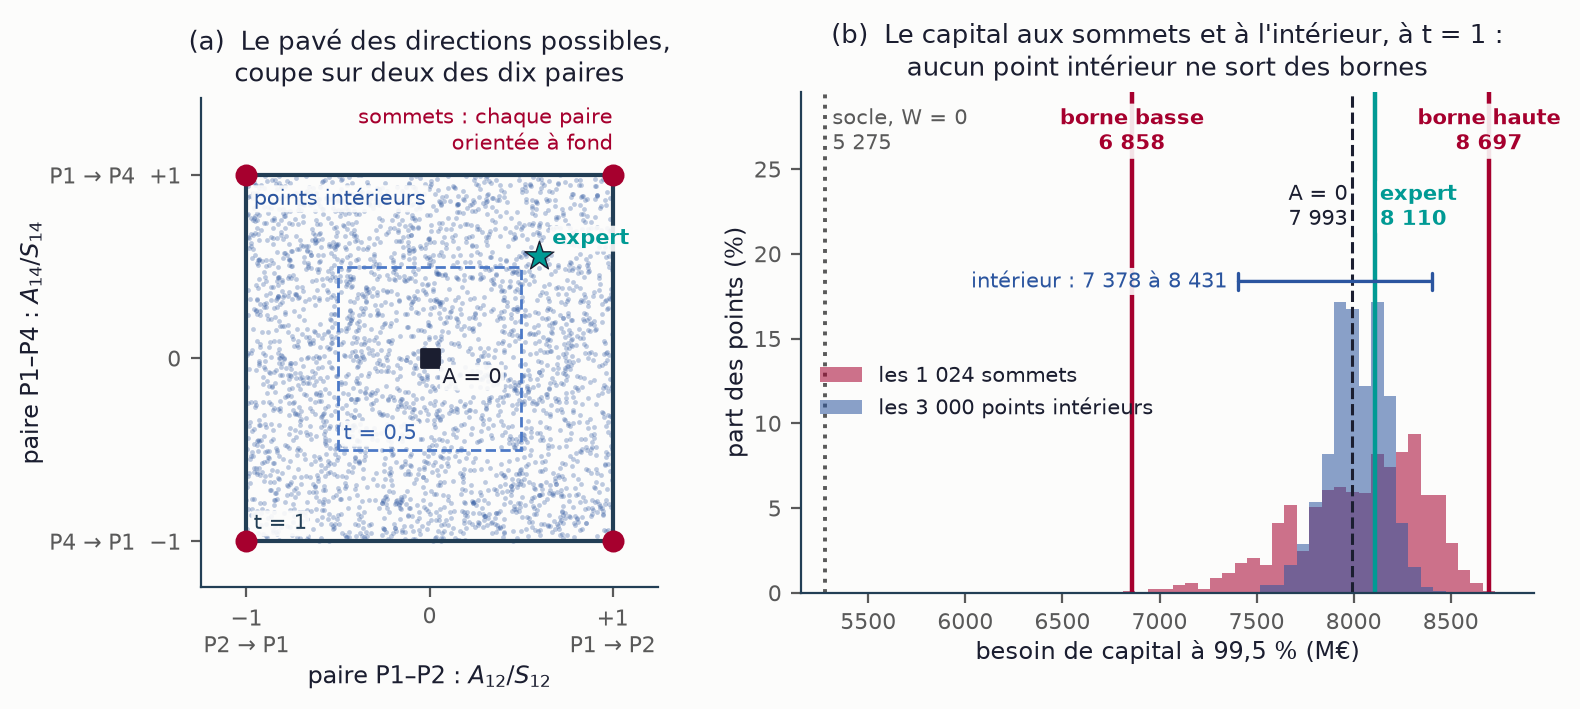
\includegraphics[width=\linewidth]{Z_pave_sommets.png}\par
  {\tiny\color{gris}(a) coupe du pavé sur deux des dix paires. (b) capital aux sommets (rouge) et aux points intérieurs (bleu).\par}
  \column{.30\textwidth}\footnotesize
  \textbf{1 · Simuler une fois}\par
  Mêmes 40\,000 années pour toutes les matrices : les écarts viennent de $W$.\par\vspace{1.5mm}
  \textbf{2 · Un capital par sommet}\par
  $\VaR_{99{,}5\,\%}(L\mid W)$ pour les 1\,024 matrices.\par\vspace{1.5mm}
  \textbf{3 · Lire la plage}\par
  Minimum et maximum sur les sommets ; aucun des 3\,000 points intérieurs n'en sort.\par\vspace{1.5mm}
  {\color{accent}\textbf{[6\,858 ; 8\,697] M€}}, largeur 1\,839 M€.\par\vspace{1mm}
  {\scriptsize\color{gris}Cascade indépendante, fréquence conforme, $g=0{,}90$ : la plage ne se compare pas directement aux capitaux par état (marche auto-évitante).\par}
  \end{columns}
  \source{rapport, § 8.1–8.2, figure 9.1. $S$ posée, fréquence conforme, $g=0{,}90$. Extrema globaux non démontrés.}
\end{frame}

\begin{frame}{Poser la matrice ou borner le capital ?}
  \suivimethode{7}{Capital}
  \framesubtitle{\ajout Deux régimes de publication, comparés sur le même socle}
  \begin{columns}[T,onlytextwidth]
    \column{.57\textwidth}\scriptsize
    \renewcommand{\arraystretch}{1.12}
    \begin{tabularx}{\linewidth}{@{}>{\bfseries}l Y Y@{}}
      \toprule
      & A : on pose $W$ & B : modèle en couches \\
      \midrule
      Sortie & Un point, 8\,110 M€ & Socle 5\,275 + bande [6\,858 ; 8\,697] \\
      \rowcolor{clair}Part insensible au sens & Aucune : tout repose sur le classeur & 79\,\% (socle 61\,\%, plancher commun aux sommets 18\,\%), à $S$ posé \\
      Panel biaisé & Déplace le besoin de 777 M€ ($10\,\%$) & La bande ne bouge pas si $S$ reste fixé \\
      \rowcolor{clair}Priorité & P1, sans marge d'erreur & Tête P1 / P4, ordre interne ouvert \\
      Sans expert & Plus de matrice complète & Exploration conditionnelle à $S$ \\
      \bottomrule
    \end{tabularx}\par\vspace{2mm}
    Sur l'ensemble admissible, P5 n'arrive jamais en tête, P3 dans moins de 10\,\% des cas ; P1 (45\,\%) et P4 (36\,\%) concentrent 81\,\% des matrices testées. Un panel d'experts servirait à les départager ; le questionnaire diffusé est resté sans réponse.
    \column{.39\textwidth}\scriptsize
    {\editorial\normalsize Niveaux selon la calibration}\par\vspace{1mm}
    \renewcommand{\arraystretch}{1.12}
    \setlength{\tabcolsep}{3pt}\begin{tabular}{@{}lrrr@{}}
      \toprule
      M€ & Socle & Bornes & $\tfrac{\text{haute}}{\text{socle}}$ \\
      \midrule
      Référence (OpRisk) & 5\,275 & [6\,858 ; 8\,697] & 1,65 \\
      Sévérité PRC & 239 & [336 ; 424] & 1,77 \\
      Fréquence $\times3$ & 11\,709 & [14\,353 ; 17\,405] & 1,49 \\
      \bottomrule
    \end{tabular}\par\vspace{1.5mm}
    La borne haute varie d'un facteur 41 entre PRC et fréquence triplée ; les rapports varient d'au plus $33\,\%$ de leur moyenne, et P1 et P4 restent en tête dans les trois calibrations.\par\vspace{1mm}
    {\color{accent}On lit donc les écarts, les rapports et les classements, pas les niveaux.}
  \end{columns}
  \source{rapport, chapitre 8 (§ 8.3 et 8.4). Capitaux du chapitre 8 : cascade indépendante ; ils ne se comparent pas directement aux capitaux par état (marche auto-évitante).}
\end{frame}

\begin{frame}{Que gagne-t-on à resserrer la direction ?}
  \suivimethode{7}{Capital}
  \framesubtitle{\ajout Degré d'ignorance $t$ et échelle de repli}
  \begin{columns}[T,onlytextwidth]
    \column{.47\textwidth}\scriptsize
    \textbf{Degré d'ignorance.} L'ensemble $\mathcal W(t)=\{S+A:\ A^\top=-A,\ |A_{jk}|\le tS_{jk},\ \rho(S+A)<1\}$ ; $t=1$ correspond aux sources publiques actuelles.\par\vspace{1mm}
    \renewcommand{\arraystretch}{1.12}
    \begin{tabular}{@{}lrrrr@{}}
      \toprule
      $t$ & 0,25 & 0,50 & 0,75 & 1 \\
      \midrule
      Largeur de la bande, M€ & 336 & 695 & 1\,083 & 1\,839 \\
      \bottomrule
    \end{tabular}\par\vspace{1mm}
    Borner l'asymétrie à la moitié de la co-occurrence réduirait la largeur de 1\,839 à 695 M€ ($-62\,\%$) : un ordre de grandeur de ce que le reporting recommandé permettrait de gagner, sans le garantir.\par\vspace{1mm}
    \textbf{Échelle de repli.} Direction écrite par l'excès de propagation propre à la source, $\mathrm{logit}\,p_{ij}=\mathrm{logit}\,p_j+u_{ij}$, que l'on limite par crans. Le rang 1 capte $74\,\%$ de la variance de la direction posée et resserre les bornes de $25\,\%$.\par\vspace{1mm}
    Au cran nul, P1 et P4 sont indiscernables (1\,051 contre 1\,052 M€), alors que 353 M€ les séparent avec la direction du classeur : \textbf{la direction départage les deux piliers prioritaires.}
    \column{.49\textwidth}
    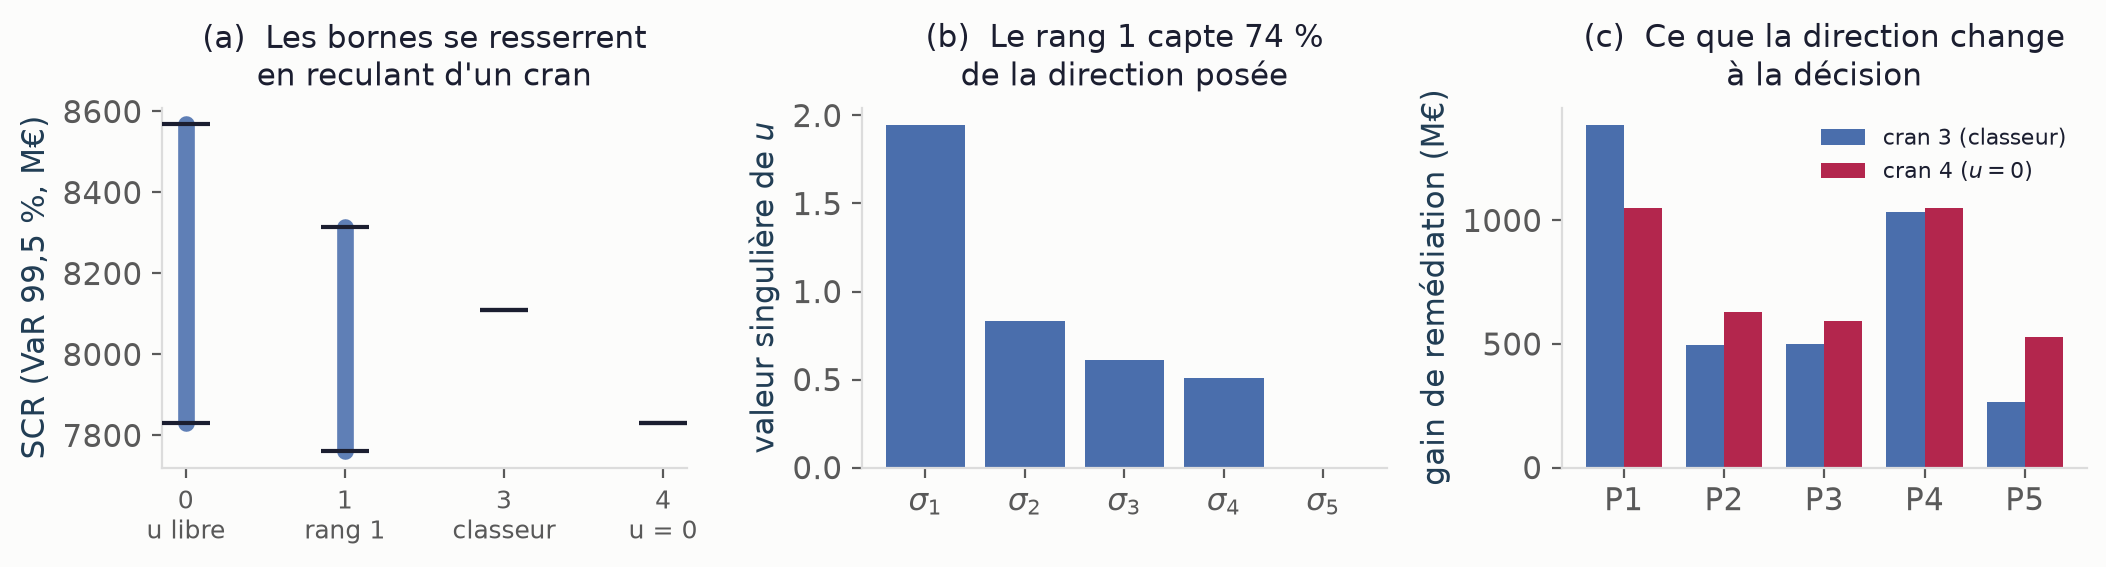
\includegraphics[width=\linewidth]{Z5_echelle_repli.png}\par
    {\tiny\color{gris}(a) Les bornes se resserrent quand la direction descend d'un cran : $u$ libre, rang 1, classeur, cran nul. (b) Valeurs singulières de la direction posée. (c) Gains de remédiation par pilier.\par}
    \scriptsize\vspace{1mm}
    Les extrema sont numériques : les 3\,000 points intérieurs tirés restent dans les bornes et 172 ascensions depuis des sommets ou des points intérieurs finissent toutes sur un sommet, mais cela n'est pas démontré.
  \end{columns}
  \source{rapport, chapitre 8 (§ 8.1, 8.2 et 8.5, figure 8.2) ; chapitre 9 (§ 9.7). Largeur : sur sommets admissibles, à $S$ posé.}
\end{frame}


% =============================================================================
\section{Résultats}
\begin{frame}{Comment mesurer l'effet de la conformité ?}
  \suivimethode{2,7}{Deux états}
  \framesubtitle{\ajout Basculer les quatre canaux ensemble, mêmes graines}
  \begin{columns}[T,onlytextwidth]
    \column{.58\textwidth}\footnotesize
    \renewcommand{\arraystretch}{1.3}
    \begin{tabularx}{\linewidth}{@{}l Y r r@{}}
      \toprule
      \textbf{Canal} & \textbf{Paramètre} & \textbf{C} & \textcolor{accent}{\textbf{NC}} \\
      \midrule
      Fréquence & $\lambda$ : incidents par an & 21,56 & \textcolor{accent}{53,62} \\
      Détection & $p_u$ : dépassement de $u$ & 0,128 & \textcolor{accent}{0,181} \\
      Propagation & $g$ : gain de $W$ & 0,45 & \textcolor{accent}{0,90} \\
      Accumulation & probabilité de choc commun & 0 & \textcolor{accent}{0,68} \\
      \bottomrule
    \end{tabularx}\par\vspace{2mm}
    \textbf{Protocole.} Même moteur, mêmes graines, même sévérité de base : seuls ces quatre paramètres changent.
    On compare $\VaR_{99{,}5\,\%}(L_{\mathrm{NC}})$ et $\VaR_{99{,}5\,\%}(L_{\mathrm{C}})$.\par\vspace{1mm}
    {\scriptsize\color{gris}Valeurs non conformes posées (multiplicateurs de scénario), non estimées.}
    \column{.38\textwidth}
    \centering
    \begin{tikzpicture}[x=1mm,y=1mm]
      \draw[filet] (0,0)--(46,0);
      \fill[gris!45] (5,0) rectangle (19,6.6);
      \fill[accent] (27,0) rectangle (41,22);
      \node[above,font=\scriptsize,text=ardoise] at (12,6.6) {6\,049 M€};
      \node[above,font=\scriptsize,text=accent] at (34,22) {20\,188 M€};
      \node[below,font=\scriptsize] at (12,0) {Conforme};
      \node[below,font=\scriptsize] at (34,0) {Non conforme};
    \end{tikzpicture}\par\vspace{1mm}
    {\editorial\fontsize{18}{19}\selectfont\color{accent}$\times\,3{,}34$}\par\vspace{.5mm}
    \raggedright\scriptsize Écart de \textbf{14\,139 M€} ; écart-type Monte-Carlo entre quatre graines : 734 M€.
    Interactions entre canaux : \textbf{35\,\%} de l'écart.\par\vspace{.5mm}
    {\color{accent}Suppose que les pertes des piliers touchés s'additionnent.}
  \end{columns}
  \source{rapport, chapitre 6 et § 9.1. Niveau illustratif ; l'amplitude dépend des paramètres posés. Tirages communs seulement entre configurations de même fréquence.}
\end{frame}

\begin{frame}{Quatre lectures de l'écart : laquelle publier ?}
  \suivimethode{2,7}{Canaux, capital}
  \framesubtitle{\ajout Lectures emboîtées de l'écart entre états}
  \begin{columns}[T,onlytextwidth]
    \column{.54\textwidth}\scriptsize
    \renewcommand{\arraystretch}{1.12}
    \begin{tabularx}{\linewidth}{@{}Y r r r r@{}}
      \toprule
      Lecture & Canaux & Conforme & Non conf. & Facteur \\
      \midrule
      Score de conformité seul, $g$ figé au niveau NC & 1 & 7\,987 & 16\,847 & 2,11 \\
      \rowcolor{clair}Fréquence + propagation (lecture B) & 2 & 6\,664 & 15\,074 & 2,26 \\
      + détection (lecture C) & 3 & 5\,932 & 16\,595 & 2,80 \\
      \rowcolor{clair}\textbf{+ accumulation P4 (quatre canaux)} & 4 & 6\,049 & 20\,188 & \textcolor{accent}{\textbf{3,34}} \\
      \bottomrule
    \end{tabularx}\par\vspace{1.5mm}
    Les quatre protocoles ne diffèrent que par le nombre de canaux relâchés. Nous publions les quatre canaux, \textbf{6\,049 $\to$ 20\,188 M€}, écart de 14\,139 M€ (écart-type de 734 M€ entre quatre graines, erreur type de la moyenne 367 M€) : c'est la seule lecture où l'état conforme l'est sur tous les canaux du modèle. Dans les autres, il propage encore comme une entité défaillante, ou sa détection ou son accumulation restent au niveau non conforme : ce sont des remédiations partielles.
    \column{.42\textwidth}\scriptsize
    {\editorial\normalsize Surcoût $\Delta_{\mathrm{DORA}}$, lecture B}\par\vspace{1mm}
    Bootstrap à deux niveaux (multiplicateurs et sévérité), graine commune ; 100\,\% des tirages positifs.\par\vspace{1mm}
    \renewcommand{\arraystretch}{1.12}
    \begin{tabular}{@{}lrr@{}}
      \toprule
      M€ & Médiane & IC à 90\,\% \\
      \midrule
      NC contre C, OpRisk & 6\,476 & [2\,940 ; 47\,368] \\
      PC contre C, OpRisk & 2\,346 & [1\,137 ; 13\,566] \\
      NC contre C, PRC & 3\,668 & [3\,201 ; 4\,094] \\
      PC contre C, PRC & 1\,257 & [1\,077 ; 1\,466] \\
      \bottomrule
    \end{tabular}\par\vspace{1mm}
    L'intervalle large côté OpRisk est la signature d'une queue d'indice $0{,}60$ ; il porte sur la lecture B. Pour l'écart à quatre canaux, seule la dispersion entre graines est publiée.\par\vspace{1mm}
    {\color{accent}Ce facteur compare deux états posés :} ce n'est pas un effet de DORA mesuré sur des entités.
  \end{columns}
  \source{rapport, chapitre 9 (§ 9.1, tableaux 9.1 et 9.2). Le facteur se compare d'une lecture à l'autre, non l'écart en euros.}
\end{frame}

\begin{frame}{Comment attribuer l'écart à chaque canal ?}
  \suivimethode{2,7}{Attribution par canal}
  \framesubtitle{\ajout Seize configurations, deux lectures d'un même canal}
  \begin{columns}[c,onlytextwidth]
    \column{.56\textwidth}
    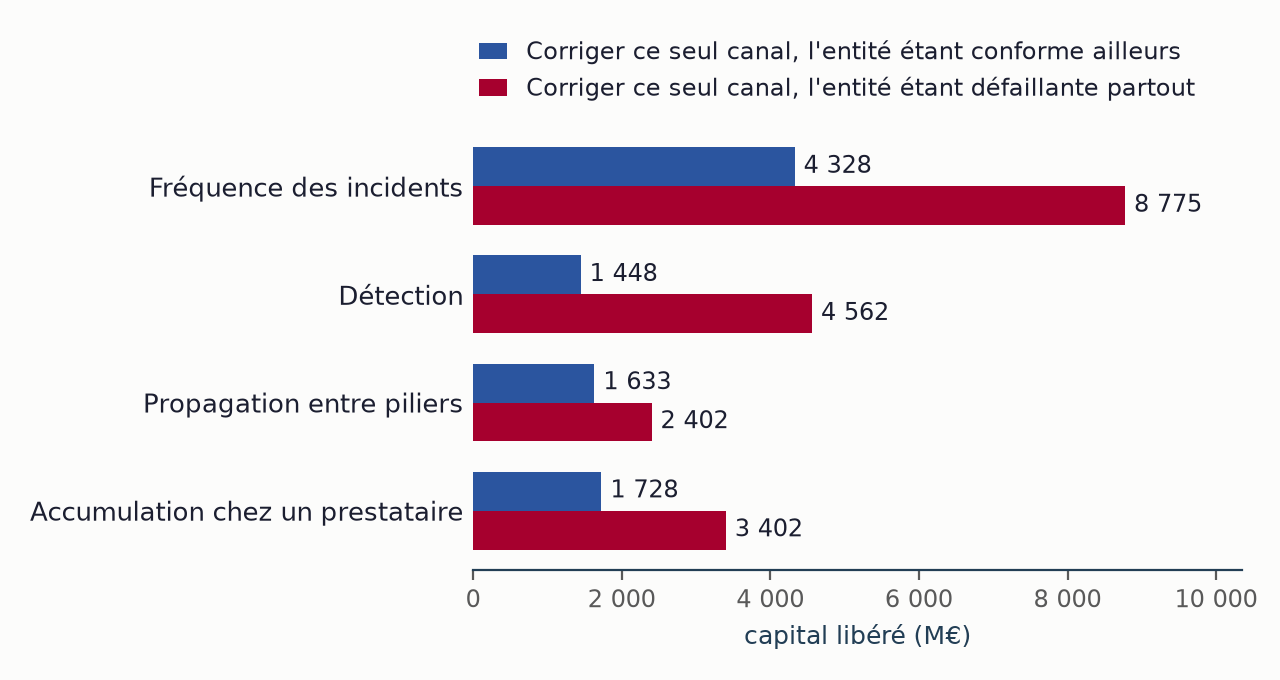
\includegraphics[width=\linewidth]{N1_canaux_note.png}
    \column{.41\textwidth}\footnotesize
    $2^4=16$ configurations, simulées avec les mêmes graines ; $V(\cdot)$ : capital de la configuration.\par\vspace{2mm}
    \textbf{Effet isolé} (depuis l'état conforme)\par
    $\Delta^{\mathrm{iso}}_c=V(\{c\})-V(\varnothing)$\par\vspace{1mm}
    \textbf{Effet de fermeture} (depuis l'état non conforme)\par
    $\Delta^{\mathrm{ferm}}_c=V(\text{tout})-V(\text{tout}\setminus\{c\})$\par\vspace{2mm}
    Fréquence : {\editorial 4\,328 M€} isolé, {\editorial\color{accent}8\,775 M€} en fermeture.
    L'écart entre les deux lectures mesure les interactions que le canal porte.\par\vspace{1mm}
    {\scriptsize\color{gris}Les effets de fermeture ne s'additionnent pas.}\par\vspace{1mm}
    {\small\color{accent}\itshape$\rightarrow$\enspace Et pour une entité donnée ?\par}
  \end{columns}
  \source{rapport, chapitre 9, figure 9.1. Gains conditionnels aux paramètres posés ; les gains de fermeture ne s'additionnent pas.}
\end{frame}

\begin{frame}{Les canaux s'additionnent-ils ?}
  \suivimethode{2,7}{Canaux, capital}
  \framesubtitle{\ajout Seize configurations : une interaction de +5\,001 M€}
  \begin{columns}[T,onlytextwidth]
    \column{.52\textwidth}
    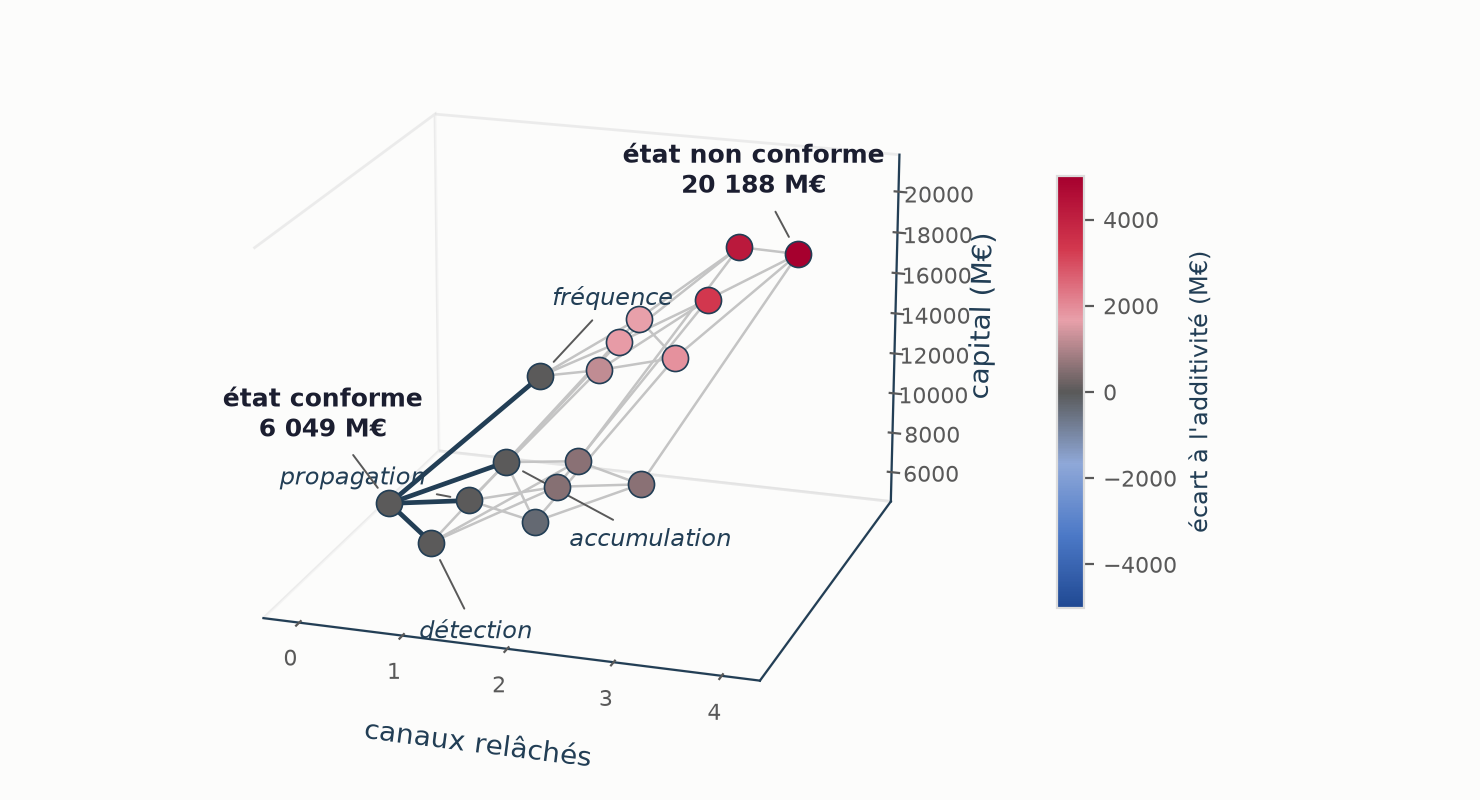
\includegraphics[width=\linewidth]{S33_treillis_canaux_3d.png}\par
    {\tiny\color{gris}Les seize configurations des quatre canaux, rangées par nombre de canaux relâchés. Hauteur : capital ; extrémités : 6\,049 et 20\,188 M€. Couleur : écart à l'additivité (+5\,001 M€ au sommet complet, $-330$ sur la seule paire négative, propagation et accumulation). Chaque arête monte.\par}
    \column{.44\textwidth}\scriptsize
    Les quatre effets isolés somment à \textbf{9\,138 M€} ; l'écart de 14\,139 les dépasse de \textcolor{accent}{\textbf{5\,001}} M€.\par\vspace{1.2mm}
    Les canaux se multiplient presque : le produit des quatre facteurs isolés vaut $3{,}47$ pour un facteur publié de $3{,}34$ ; un modèle purement multiplicatif donnerait 5\,813 M€ d'interaction. Elle correspond à ce produit plus qu'à un effet propre de la cascade.\par\vspace{1.2mm}
    \textbf{Une seule paire est négative :} propagation et accumulation, deux canaux de co-occurrence, sont substituts, non compléments.\par\vspace{1.2mm}
    \renewcommand{\arraystretch}{1.12}
    \begin{tabular}{@{}lr@{}}
      \toprule
      Fréquence seule & 10\,377 M€ ($\times1{,}72$) \\
      Les trois autres canaux réunis & 11\,413 M€ ($\times1{,}89$) \\
      \bottomrule
    \end{tabular}\par\vspace{1mm}
    Toute cible sous le premier seuil se produit par un canal unique ; toute cible au-delà du second \textbf{exige la fréquence}. Aucun autre canal seul n'atteint 8\,000 M€.
  \end{columns}
  \source{rapport, chapitre 9 (§ 9.1, § 9.5, figure 9.2). Test de résistance inverse : la monotonie rend croissant l'ensemble des configurations atteignant une cible.}
\end{frame}

\begin{frame}{Quel pilier supporte le surcoût ?}
  \suivimethode{5,7}{Cascade, capital}
  \framesubtitle{\ajout Valeur de Shapley et allocation d'Euler}
  \begin{columns}[T,onlytextwidth]
    \column{.54\textwidth}\scriptsize
    \renewcommand{\arraystretch}{1.12}
    \begin{tabular}{@{}l r r r r r@{}}
      \toprule
      & \multicolumn{3}{c}{OpRisk} & \multicolumn{2}{c}{PRC} \\
      \cmidrule(lr){2-4}\cmidrule(lr){5-6}
      Pilier & marginal & $\varphi_j$ & part & $\varphi_j$ & part \\
      \midrule
      P1 gouvernance & 3\,481 & 3\,717 & 34,0\,\% & 1\,608 & 32,4\,\% \\
      \rowcolor{clair}P4 tiers & 2\,658 & 2\,810 & 25,7\,\% & 1\,252 & 25,3\,\% \\
      P2 incidents & 1\,634 & 1\,867 & 17,1\,\% & 920 & 18,6\,\% \\
      \rowcolor{clair}P3 tests & 1\,094 & 1\,484 & 13,6\,\% & 738 & 14,9\,\% \\
      P5 partage & 665 & 1\,048 & 9,6\,\% & 438 & 8,8\,\% \\
      \midrule
      somme & 9\,531 & 10\,927 & 100\,\% & 4\,957 & 100\,\% \\
      \bottomrule
    \end{tabular}\par\vspace{1mm}
    {\tiny M€ ; périmètre financier étudié, trois canaux (fréquence, propagation, détection), base conforme 6\,085 du moteur par pilier.\par}\vspace{1mm}
    Le classement de Shapley reproduit le classement ROOT, en partie mécaniquement (amorces 30/27/18/15/9\,\%). La part de P1, $34\,\%$, excède toutefois sa part d'amorce de $30\,\%$ : c'est l'effet propre de la propagation, P1 étant l'émetteur le plus fort.
    \column{.42\textwidth}\scriptsize
    {\editorial\normalsize Pourquoi une règle additive ?}\par\vspace{1mm}
    Les surcoûts isolés ne somment pas au total. Sur la VaR OpRisk, l'interaction entre piliers n'est pas de signe résolu : de $-137$ à $+1\,395$ M€ sur six graines, positive quatre fois. Elle ne s'additionne pas aux $+5\,001$ M€ entre canaux : deux axes de décomposition.\par\vspace{1.5mm}
    {\editorial\normalsize Euler : où se loge la queue}\par\vspace{1mm}
    Les contributions $C_j=\mathbb E[L_j\mid L\ge\mathrm{VaR}]$ somment à la TVaR, non au quantile. PRC : allocation presque plate (23, 23, 20, 18, 17\,\%). OpRisk : parts moyennes stables mais allocation de queue instable, la variance étant infinie.\par\vspace{1mm}
    Rapport $\mathrm{TVaR}/\mathrm{VaR}\approx2{,}1$ contre l'asymptote $1/(1-\xi)=2{,}5$. Sous PRC non plafonnée, $\hat\xi=1{,}033>1$ : l'espérance est infinie, la mesure de queue n'existe pas.
  \end{columns}
  \source{rapport, chapitre 9 (§ 9.2 et 9.3, tableau 9.3). Le capital publié est le quantile non centré ; aucune grandeur de couverture n'est une TVaR.}
\end{frame}

\begin{frame}{Dans quel ordre remédier ?}
  \suivimethode{5,7}{Cascade, capital}
  \framesubtitle{\ajout Cent vingt ordres énumérés, un ordre optimal}
  \begin{columns}[T,onlytextwidth]
    \column{.50\textwidth}\footnotesize
    \textbf{Ordre optimal.} Sous budget contraint, un pilier remédié à la fois : P1 $\to$ P4 $\to$ P2 $\to$ P3 $\to$ P5, égal à l'ordre ROOT et distinct de l'ordre glouton par valeur d'accélération. L'écart de capital intégré entre le pire ordre et l'optimal atteint $21\,\%$ : les interactions de cascade imposent de raisonner sur l'horizon entier.\par\vspace{1.5mm}
    \textbf{Trajectoire.} Depuis une répartition supposée des états (NC 35\,\%, PC 35\,\%, C 30\,\%), en lecture B, le capital OpRisk passe de 10\,752 à 7\,041 M€ en cinq ans. Le surcoût résiduel tend vers zéro ; son intégrale, à un coût de capital près, est le coût de portage de la non-conformité.\par\vspace{1.5mm}
    \textbf{Invariance.} L'ordre optimal ne dépend que des SCR par configuration, donc pas des taux de transition de la chaîne de Markov.
    \column{.46\textwidth}\footnotesize
    {\editorial\normalsize Robustesse de la priorité}\par\vspace{1.5mm}
    Sur l'ensemble admissible, P1 arrive premier dans $43{,}6\,\%$ des configurations et P4 dans $37{,}7\,\%$, avec un regret maximal de $1{,}5\,\%$ : \textbf{presque à égalité}. P5 n'arrive jamais en tête.\par\vspace{1.5mm}
    Les rapports post-incident pouvant sur-attribuer à la gouvernance, on dégrade l'émission de P1 par $W_{1k}\to(1-a)W_{1k}$ : le classement tient jusqu'à $a=0{,}25$, puis bascule vers P4 à $a=0{,}50$. Même à $a=1$, le niveau ne perd que $24{,}8\,\%$.\par\vspace{1.5mm}
    Sans la direction (partie antisymétrique supprimée), P1 et P4 ne se distinguent plus.\par\vspace{1mm}
    {\color{accent}Donc :} la tête, P1 et P4, est robuste ; l'ordre entre les deux dépend de la direction posée.
  \end{columns}
  \source{rapport, chapitre 9 (§ 9.4, 9.5 et 9.6) et chapitre 10 (§ 10.1).}
\end{frame}

\begin{frame}{Quel cadre exprime l'effet de la conformité ?}
  \suivimethode{5,7}{Cascade, capital}
  \framesubtitle{\ajout Formule Standard, copule, cascade dirigée}
  \begin{columns}[T,onlytextwidth]
    \column{.46\textwidth}\scriptsize
    \renewcommand{\arraystretch}{1.2}
    \begin{tabularx}{\linewidth}{@{}Y r r@{}}
      \toprule
      Cadre & $\Delta$ capital C$\to$NC & Part de l'effet \\
      \midrule
      Formule Standard (Solvabilité II) & 0 M€ & 0\,\% \\
      \rowcolor{clair}LDA-copule (dépendance symétrique) & 6\,760 M€ & 62\,\% \\
      Cascade dirigée & 10\,927 M€ & 100\,\% (référence) \\
      \bottomrule
    \end{tabularx}\par\vspace{1.5mm}
    {\tiny Périmètre financier étudié, trois canaux, accumulation exclue, protocole du tableau 9.3.\par}\vspace{1.5mm}
    La charge de risque opérationnel de la Formule Standard ne dépend que du volume : identique pour une entité exemplaire et pour une entité défaillante sur DORA. La copule capte $62\,\%$ de l'effet, par la fréquence et la détection, mais manque la propagation.
    \column{.50\textwidth}\scriptsize
    {\editorial\normalsize Le niveau n'identifie pas la dépendance}\par\vspace{1mm}
    À corrélation calée, la copule gaussienne retombe sur le capital de la cascade : $+0{,}1\,\%$ sur une graine, $+4{,}8\,\%$ en moyenne sur quatre, sous son propre bruit. En queue lourde, le quantile annuel tient à la perte unique dominante.\par\vspace{1mm}
    La Student ($\nu=4$) le surestime de $17\,\%$ en forçant des co-extrêmes que la cascade ne produit pas : 2,28 piliers extrêmes par année de queue contre 1,12.\par\vspace{1.5mm}
    {\editorial\normalsize Mais une intervention, pas une corrélation}\par\vspace{1mm}
    Basculer un pilier en non-conformité est une intervention : la copule y donne un surcoût inférieur de $38\,\%$ (6\,760 contre 10\,927 M€), son interaction moyenne est nulle par construction quand la cascade en produit $+560$ M€, et la priorité qu'elle implique s'inverse sur P2 et P3. Sa dépendance ne durcit pas quand la conformité se dégrade, alors que c'est le canal de propagation que la non-conformité déplace.
  \end{columns}
  \source{rapport, chapitre 9 (§ 9.8 et 9.9, tableau 9.4). Le préprint de cascade climatique (Karimi et al., 2026) emploie le même protocole de comparaison.}
\end{frame}


% =============================================================================
\section{Échelle d'entité}
\begin{frame}{Comment passer du marché à une entité ?}
  \suivimethode{8}{Entité}
  \framesubtitle{\ajout Partager la fréquence du secteur selon la taille ; lire la sévérité à la taille}
  \begin{columns}[T,onlytextwidth]
    \column{.54\textwidth}\scriptsize
    \setlength{\abovedisplayskip}{.5mm}\setlength{\belowdisplayskip}{.5mm}
    \textbf{1 · Une part de la fréquence du secteur}
    \[\lambda(A)=\Lambda\,\frac{A^{\,b_\lambda}}{\overline{\sum_{j\in\mathcal J_y}A_j^{\,b_\lambda}}}\]
    $\Lambda=79{,}0$ : nombre moyen d'incidents annuels du panel OpRisk.
    $\mathcal J_y$ : firmes actives l'année $y$, 808 en moyenne ; la barre est la moyenne annuelle de la somme.
    Les $\lambda(A_j)$ somment à $\Lambda$ \textbf{en moyenne annuelle}. $A$ : actifs de l'entité.\par\vspace{1mm}
    \textbf{2 · Une sévérité lue à la taille}
    \[m(A)=\Big(\frac{A}{A_m}\Big)^{b},\qquad b=0{,}087\]
    $A_m$ : taille médiane des pertes retenues ; $m=0{,}854$ à la taille de l'entité notionnelle.\par\vspace{1mm}
    \textbf{3 · Perte et capital de l'entité}
    \[X=m(A)\sum_{k\in S_a}Y_k,\qquad \mathcal B(A)=\mathrm{VaR}_{99{,}5\,\%}\Big(\sum_{n=1}^{N}X_n\Big)\]
    $N$ : binomiale négative de moyenne $\lambda(A)$ ; $S_a$ : piliers touchés depuis l'amorce $a$ ; $Y_k$ : sévérités GPD. $W$ et moteur inchangés.
    \column{.42\textwidth}\scriptsize
    {\editorial\normalsize Un seul exposant règle la taille}\par\vspace{1mm}
    $b_\lambda$ fixe la part de fréquence que prend une entité selon ses actifs. Trois lectures sont publiées :\par\vspace{1mm}
    \renewcommand{\arraystretch}{1.15}
    \begin{tabularx}{\linewidth}{@{}>{\bfseries}l r Y@{}}
      \toprule
      Lecture & $b_\lambda$ & Statut \\
      \midrule
      Registre & 0,074 & estimé sur OpRisk \\
      \rowcolor{clair}Centrale & 0,27 & posé : $\sqrt{0{,}074}$ \\
      Proportionnelle & 1 & convention de la tarification à l'exposition \\
      \bottomrule
    \end{tabularx}\par\vspace{1.5mm}
    La lecture centrale est le milieu géométrique des deux lectures extrêmes. \textcolor{accent}{Elle est posée, non estimée} : aucune donnée du dépôt ne sépare les deux extrêmes.\par\vspace{1.5mm}
    L'ancienne méthode du mémoire est le cas $b_\lambda=0{,}074$ : le partage la reproduit à $0{,}11\,\%$ près.
  \end{columns}
  \source{rapport, chapitre 9 (§ 9.10, équation 9.1). Script 130 : partage de l'exposition, identité de somme et reproduction contrôlées.}
\end{frame}

\begin{frame}{Que dit la donnée de la taille ?}
  \suivimethode{8}{Entité}
  \framesubtitle{\ajout Le registre enregistre ce qui est déclaré, pas l'exposition}
  \begin{columns}[T,onlytextwidth]
    \column{.50\textwidth}\footnotesize
    {\editorial\normalsize Aucun effet de taille dans le registre}\par\vspace{1.5mm}
    Sur les \textbf{521 pertes} dont les actifs sont connus, la pente de la perte sur la taille est nulle ou négative : $-0{,}07$ (erreur-type $0{,}03$), et $-0{,}13$ aux quantiles 75 et 90\,\%. Elle le reste parmi les firmes de plus de 50 Md\$ d'actifs.\par\vspace{1.5mm}
    La part des pertes au-delà du seuil vaut $13\,\%$ dans le premier cinquième des actifs et $4\,\%$ dans le dernier. \textbf{12 des 66} pertes au-delà du seuil viennent de firmes de moins de 1 Md\$ d'actifs.\par\vspace{1.5mm}
    Spearman entre perte et taille : $0{,}159$ (chiffre d'affaires), $0{,}139$ (effectif), $0{,}068$ (actif total), sur 33\,769 pertes.
    \column{.46\textwidth}\footnotesize
    {\editorial\normalsize Ce qu'on en conclut}\par\vspace{1.5mm}
    Un exposant estimé sur ce registre ne dit rien de ce qu'une entité plus grande risque : grandes firmes et petites déclarent des pertes comparables parce que la base recense des pertes rendues publiques.\par\vspace{1.5mm}
    Un même niveau pour un grand groupe et pour une petite entité n'est donc pas défendable. Nous publions \textbf{trois lectures}, de $b_\lambda=0{,}074$ à $b_\lambda=1$, avec la lecture centrale $b_\lambda=0{,}27$ comme repère.\par\vspace{1.5mm}
    {\color{accent}Le choix du milieu géométrique est une décision de modélisation, déclarée comme telle ;} il se juge à l'ordre qu'il produit, pas à son niveau.\par\vspace{1.5mm}
    {\scriptsize Valeurs en dollars des bases OpRisk ; le moteur convertit au taux fixe de 0,92.\par}
  \end{columns}
  \source{rapport, chapitre 9 (§ 9.10) et chapitre 3 (§ 3.8.4). La faible élasticité de sévérité (0,087, [0,026 ; 0,148]) va dans le même sens sans le confirmer au sens statistique.}
\end{frame}

\begin{frame}{Le besoin suit-il la taille de l'entité ?}
  \suivimethode{8}{Entité}
  \framesubtitle{\ajout Trois lectures, sept entités, en M€}
  \scriptsize
  \renewcommand{\arraystretch}{1.08}
  \setlength{\tabcolsep}{4pt}
  \begin{tabularx}{\linewidth}{@{}l r r r r r@{}}
    \toprule
    \textbf{Entité} & \textbf{Actifs} & \textbf{SCR publié} & \textbf{Registre} & \textbf{Centrale} & \textbf{Proportionnelle} \\
    \midrule
    Petite entité (posée) & 500 & --- & 86 [63 ; 93] & nul & nul \\
    \rowcolor{clair}Assureur non-vie A & 2\,319 & 425 & 112 [88 ; 122] & nul [0 ; 15] & nul \\
    Assureur non-vie B & 5\,305 & 812 & 136 [104 ; 146] & 35 [23 ; 40] & nul \\
    \rowcolor{clair}\textit{Entité notionnelle} & 19\,231 & --- & 169 [132 ; 183] & 99 [76 ; 109] & nul \\
    Assureur vie C & 37\,845 & 1\,587 & 196 [149 ; 213] & 141 [110 ; 156] & nul \\
    \rowcolor{clair}Assureur vie D & 309\,800 & 14\,800 & 294 [233 ; 316] & 347 [277 ; 371] & 189 [142 ; 204] \\
    Grand groupe (posé) & 2\,400\,000 & --- & 398 [318 ; 428] & \textcolor{accent}{\textbf{690 [561 ; 738]}} & 1\,371 [1\,137 ; 1\,465] \\
    \bottomrule
  \end{tabularx}
  {\tiny\color{gris}Point à la matrice d'expert, bande sur les 1\,024 sommets admissibles. « Nul » : le quantile à 99,5\,\% est nul (taille de bascule). Les tailles de la petite entité et du grand groupe sont posées ; aucune n'est une entité observée.\par}
  \vspace{1.5mm}
  \begin{columns}[T,onlytextwidth]
    \column{.47\textwidth}\scriptsize
    {\color{accent}\textbf{Pourquoi l'assureur D ne vaut-il que 2,6 fois A en lecture du registre ?}}\par\vspace{.5mm}
    Les actifs de D sont 134 fois ceux de A, mais les exposants du registre sont faibles : $134^{0{,}074}\approx1{,}44$ sur la fréquence et $134^{0{,}087}\approx1{,}53$ sur la sévérité. Le registre mesure ce qui est déclaré, pas l'exposition.
    \column{.49\textwidth}\scriptsize
    {\color{accent}\textbf{Ce que change la lecture centrale.}}\par\vspace{.5mm}
    A passe sous la taille de bascule (besoin nul) et D vaut 347 ; le grand groupe vaut \textbf{19,5 fois} l'assureur B pour un facteur 452 sur les actifs, contre 2,9 en lecture du registre. Besoin central rapporté au SCR publié : $4{,}3\,\%$, $8{,}9\,\%$ et $2{,}3\,\%$ pour B, C et D.
  \end{columns}
  \source{rapport, chapitre 9 (§ 9.11, script 130). Assureurs anonymisés, bilans SFCR 2024 ; état de conformité supposé, écart entre états de $+41\,\%$ à $+49\,\%$ à toutes les tailles en lecture du registre.}
\end{frame}

\begin{frame}{Sous quelle taille le besoin est-il nul ?}
  \suivimethode{7,8}{Capital, entité}
  \framesubtitle{\ajout La taille de bascule du quantile à 99,5\,\%}
  \begin{columns}[T,onlytextwidth]
    \column{.50\textwidth}\footnotesize
    Si la probabilité annuelle de charge de queue positive est sous $0{,}5\,\%$, le quantile à 99,5\,\% est nul.
    Plus de $99{,}5\,\%$ des années ont une perte nulle. Un incident compté peut avoir une perte nulle :
    la sévérité est nulle sous le seuil.\par\vspace{1mm}
    \renewcommand{\arraystretch}{1.25}
    \begin{tabular}{@{}lr@{}}
      \toprule
      Lecture & Taille de bascule \\
      \midrule
      Centrale ($b_\lambda=0{,}27$) & \textcolor{accent}{\textbf{2\,517 M€}} d'actifs \\
      Proportionnelle ($b_\lambda=1$) & \textcolor{accent}{\textbf{141\,079 M€}} d'actifs \\
      \bottomrule
    \end{tabular}\par\vspace{2mm}
    Pour A et la petite entité, le quantile est nul à 99,5\,\% et à tout niveau inférieur.
    Lire le risque à un niveau plus élevé ou par une autre mesure de queue explicitée.
    En lecture proportionnelle, seuls les deux plus grands acteurs gardent un besoin positif.
    \column{.46\textwidth}\footnotesize
    {\editorial\normalsize Une limite de lecture du quantile}\par\vspace{1.5mm}
    La bascule indique où le quantile devient positif dans ce scénario ; elle ne détermine pas
    le domaine de validité statistique du modèle. Les tailles sont obtenues sur une seule graine : ordres de grandeur.\par\vspace{1.5mm}
    Un critère conventionnel de poids (10\,\% du SCR total) situe un autre seuil entre 37\,845 et 309\,800 M€ d'actifs ;
    l'entité notionnelle, à 19\,231 M€, est en dessous. Le levier propre, de $4{,}2$ à $18{,}3\,\%$, module ce repère.\par\vspace{1mm}
    L'élasticité corrige l'échelle de la sévérité, mais sa forme reste celle de grandes institutions financières.\par\vspace{1.5mm}
    {\color{accent}Les 169 M€ restent une extrapolation d'ordre de grandeur,} dont rien ne garantit qu'elle majore le besoin réel.
  \end{columns}
  \source{rapport, chapitre 9 (§ 9.11) ; script 130, section 4. La thèse concerne un rapport entre états, qui survit à une erreur de niveau commune aux trois états.}
\end{frame}

\begin{frame}{Le même modèle lu à plusieurs échelles}
  \suivimethode{7,8}{Capital, entité}
  \framesubtitle{\etabli Seules la fréquence d'amorce et l'échelle de sévérité changent}
  \begin{columns}[T,onlytextwidth]
    \column{.55\textwidth}\scriptsize
    \renewcommand{\arraystretch}{1.15}
    \setlength{\tabcolsep}{3pt}
    \begin{tabular}{@{}l r r r r@{}}
      \toprule
      Lecture & $\lambda$ (an$^{-1}$) & Sévérité & SCR 99,5\,\% & Perte moy. \\
      \midrule
      Périmètre financier étudié & 21,56 & $\times1$ & 8\,123 & 983 \\
      Seuil « $\ge10$ événements » & 0,210 & $\times1$ & 488 & 9,7 \\
      Seuil « toutes firmes » & 0,100 & $\times1$ & 229 & 4,6 \\
      $\lambda$ lu à la taille de la cible & 0,092 & $\times1$ & 198 & 4,3 \\
      \textbf{Les deux canaux composés} & \textbf{0,092} & $\boldsymbol{\times0{,}854}$ & \textcolor{accent}{\textbf{169}} & 3,6 \\
      \bottomrule
    \end{tabular}\par\vspace{1mm}
    {\tiny Montants en M€. La dernière ligne prend fréquence et sévérité à la taille de l'entité notionnelle, en lecture du registre ; elle porte les 169 M€ cités dans les chapitres précédents.\par}\vspace{1.5mm}
    Diviser $\lambda$ par 235 divise la perte moyenne par 270, mais le capital par 48 seulement : le quantile extrême dépend du plus grand sinistre.
    \column{.41\textwidth}\scriptsize
    {\editorial\normalsize Ce qui fait varier l'entité}\par\vspace{1.5mm}
    \textbf{Matrice} : bande de $[131{,}5\,;183{,}3]$ M€ sur les 1\,024 sommets ; elle ne traduit que l'ignorance de la direction (largeur 51,7 M€).\par\vspace{1.2mm}
    \textbf{Queue} : $\xi\in[0{,}304\,;0{,}831]$ fait varier le besoin de 140,9 à 191,6 M€, soit 51,5 M€.\par\vspace{1.2mm}
    \textbf{Propagation} : $g=0{,}45\,/\,0{,}68\,/\,0{,}90$ donne 116, 143 puis 169 M€, soit $+45\,\%$ ; le repère forfaitaire reste à 450 M€.\par\vspace{1.5mm}
    {\color{accent}Le chiffre d'entité est une bande, non un point :} le niveau est illustratif, l'ordre et l'écart se lisent.
  \end{columns}
  \source{rapport, chapitre 9 (§ 9.10, tableau 9.5 et figure 9.3). Repère forfaitaire de la Formule Standard : environ 450 M€.}
\end{frame}

\begin{frame}{Comment détenir ou transférer ce capital ?}
  \suivimethode{7,8}{Capital, entité}
  \framesubtitle{\ajout Capital total, coût de détention, traité en excès de perte}
  \begin{columns}[T,onlytextwidth]
    \column{.50\textwidth}\scriptsize
    \setlength{\abovedisplayskip}{.5mm}\setlength{\belowdisplayskip}{.5mm}
    \textbf{Agrégation.} Le risque opérationnel n'entre pas dans la matrice de corrélation du BSCR. Pour un écart $D$ :
    \[\Delta_{\text{additif}}=D,\qquad \Delta_\rho=\sqrt{\mathrm{BSCR}^2+2\rho\,\mathrm{BSCR}\,D+D^2}-\mathrm{BSCR}\]
    \renewcommand{\arraystretch}{1.1}
    \setlength{\tabcolsep}{3pt}
    \begin{tabular}{@{}lrrr@{}}
      \toprule
      & $D$ (M€) & $\Delta_\rho/D$ ($\rho=0{,}25$) & additif / corrélé \\
      \midrule
      Non-vie A & 34,9 & 29,4\,\% & 3,41 \\
      Non-vie B & 44,4 & 27,7\,\% & 3,62 \\
      Vie C & 62,7 & 27,4\,\% & 3,65 \\
      Vie D & 86,0 & 25,4\,\% & 3,94 \\
      \bottomrule
    \end{tabular}\par\vspace{1mm}
    $D$ est celui du seul canal de contagion, un plancher. À $\rho=0{,}25$ (posé), un euro d'écart pèse trois à quatre fois plus en convention additive qu'en corrélée : ce n'est pas une économie reconnue par le régulateur.
    \column{.46\textwidth}\scriptsize
    \textbf{Détention.} Un SCR coûte chaque année $\mathrm{CoC}\times\mathrm{SCR}$ : 6\,\%, puis 4,75\,\% au 30 janvier 2027 (directive (UE) 2025/2). Les 169 M€ pour 3,6 M€ de perte moyenne donnent un multiple de 47, contre 8,3 au secteur.\par\vspace{1mm}
    \textbf{Transfert.} Un traité en excès de perte de portée $\ell$ cède $\min(L,\ell)$ ; le coût de financement est minimal en $\ell^\star=\mathrm{SCR}=169$ M€ : de 8,0 à 2,9 M€ par an ($-64\,\%$) ; pertes conservées comprises, de 11,67 à 5,12 ($-56\,\%$).\par\vspace{1mm}
    {\color{accent}Contrat idéal :} capacité, exclusions et contrepartie le réduisent. Le transfert reste préférable tant que moins de $64\,\%$ de la portée achetée reste sans allègement de capital ($81{,}5\,\%$ pertes conservées comprises). Si la conformité ramène $\lambda$ de 0,092 à 0,046 (valeur posée), ce coût optimal baisse de $60\,\%$.
  \end{columns}
  \source{rapport, chapitre 9 (§ 9.12 et 9.13). Ratio de sinistralité de 48,5\,\% ; prime d'environ 2,1 fois la perte attendue. Le BSCR n'étant pas publié, il est minoré.}
\end{frame}

\begin{frame}{Un directeur des risques face à ces résultats}
  \suivimethode{7,8}{Capital, entité}
  \framesubtitle{\ajout Six questions, six réponses de solidité inégale}
  \scriptsize
  \renewcommand{\arraystretch}{1.12}
  \begin{tabularx}{\linewidth}{@{}>{\bfseries}p{.20\linewidth} Y p{.07\linewidth}@{}}
    \toprule
    Question & Réponse chiffrée & Section \\
    \midrule
    Quel besoin de capital au titre de DORA ? & 169 M€ à l'état non conforme, extrapolation d'ordre de grandeur, dans une bande de $[131{,}5\,;183{,}3]$ M€. Le repère forfaitaire, 450 M€, ne dépend pas de l'état. & § 9.10 \\
    \rowcolor{clair}Que change la conformité ? & Aux trois valeurs de $g$ (0,45, 0,68, 0,90), le besoin passe de 116 à 143 puis 169 M€, soit $+45\,\%$ par le seul canal de propagation. Le forfait reste à 450 M€. & § 9.10 \\
    Ce niveau est-il fiable ? & Non, c'est une extrapolation. Au levier médian ($10{,}0\,\%$), le SCR de l'entité serait de 1\,932 M€ et le besoin n'en représenterait que $9\,\%$. & § 9.11 \\
    \rowcolor{clair}Combien coûte de le détenir ? & De 8,0 à 10,1 M€ par an selon le taux, soit 2,2 à 2,8 fois la sinistralité attendue. Si la conformité divise $\lambda$ par deux (posé), le besoin tombe de 169 à 43 M€. & § 9.13 \\
    Peut-on le transférer ? & Un traité en excès de perte de portée 169 M€ ramène le coût de 8,0 à 2,9 M€ par an ($-64\,\%$ ; $-56\,\%$ pertes conservées comprises) : gain d'un contrat idéal. & § 9.13 \\
    \rowcolor{clair}Par quel pilier commencer ? & P1, puis P4, P2, P3 et P5 ; P1 et P4 presque à égalité (43,6\,\% et 37,7\,\%). Écart de capital intégré entre le pire ordre et l'optimal : $21\,\%$. & § 9.5 \\
    \bottomrule
  \end{tabularx}
  \vspace{1.5mm}
  \footnotesize\textcolor{accent}{La première réponse est un niveau, extrapolé ; la dernière est un ordre, établi à l'échelle du secteur.} Le même directeur côté capital total : pour l'assureur non-vie A, le besoin de 112 M€ ($[88\,;122]$, 26,4\,\% de son SCR publié de 425 M€) est reconnu à $29{,}4\,\%$ pour l'écart de contagion (34,9 M€).
  \source{rapport, chapitre 9 (§ 9.14). Ces réponses supposent connu l'état de conformité, qu'aucune entité ne publie : une exposition sous un état supposé, pas une non-conformité constatée.}
\end{frame}


% =============================================================================
\section{Limites}
\begin{frame}{Que tient, que ne tient pas ?}
  \suivimethode{}{}
  \framesubtitle{\ajout Synthèse de robustesse : ce qu'on fait varier, l'effet mesuré, le verdict}
  \scriptsize
  \renewcommand{\arraystretch}{1.0}
  \begin{tabularx}{\linewidth}{@{}>{\raggedright\arraybackslash}p{.27\linewidth} Y Y c@{}}
    \toprule
    Conclusion & Ce qu'on fait varier & Effet mesuré & Verdict \\
    \midrule
    $\Delta_{\mathrm{DORA}}$ positif, de plusieurs milliers de M€ & Source de sévérité (OpRisk / PRC) ; copule ($\theta\in[1,4]$) & Facteur $\sim1{,}9$ entre sources ; $<1{,}4\,\%$ sur $\theta$ & \textsc{robuste} \\
    \rowcolor{clair}Priorité P1 puis P4 & Cadre de dépendance ; branchement contre marche & P1 et P4 en tête partout ; capital $\pm4\,\%$ & \textsc{robuste} \\
    L'asymétrie de $W$ décide de l'ordre P1 / P4 & Partie antisymétrique supprimée ; placebo & Sans la direction, P1 et P4 ne se distinguent plus & \textsc{assumé} \\
    \rowcolor{clair}Les lois du socle prédisent une période non vue & Origine glissante, douze années & Couverture $91{,}7\,\%$ contre $75{,}0\,\%$ ; queue non rejetée ; peu de puissance & \textsc{assumé} \\
    \rowcolor{clair}Fréquence indépendante de la période Hackmageddon & Quatre jeux de parts, 2025--2026 & $2{,}318$ à $2{,}471$ contre $2{,}487$ ($6{,}8\,\%$ au plus) & \textsc{robuste} \\
    Le capital réagit à la conformité & Score $q$, gain $g\in[0{,}05\,;0{,}90]$ & Facteur $3{,}34$ ; $\times1{,}6$ sur la plage de $g$ & \textsc{voulu} \\
    \rowcolor{clair}Le besoin est une distribution large & Incertitude de paramètre & Facteur $\sim2{,}5$ sur le quantile d'un sinistre & \textsc{assumé} \\
    \rowcolor{clair}Le niveau de sévérité ne tient pas hors échantillon & Une année à la fois & Quantiles dépassés trois fois trop souvent ; dérive $\ge+16{,}9\,\%$ & \textsc{assumé} \\
    Le signe de $\Delta$ ne dépend pas de l'additivité & Exposant $\theta\in[0{,}70\,;1{,}30]$ & Écart de 9\,706 à 20\,487 M€ : signe et ordre conservés, amplitude non & \textsc{assumé} \\
    \bottomrule
  \end{tabularx}
  \vspace{1mm}
  {\tiny\color{gris}\textsc{robuste} : la conclusion tient aux variantes testées. \textsc{assumé} : choix déclaré dont l'effet est mesuré. \textsc{voulu} : propriété recherchée par la construction.\par}
  \source{rapport, chapitre 10 (§ 10.1).}
\end{frame}

\begin{frame}{L'incertitude se répartit sur trois étages}
  \suivimethode{}{}
  \framesubtitle{\ajout Paramètre, identification, modèle : lus sur la même charge annuelle}
  \begin{columns}[T,onlytextwidth]
    \column{.50\textwidth}\footnotesize
    \renewcommand{\arraystretch}{1.2}
    \begin{tabularx}{\linewidth}{@{}Y r r@{}}
      \toprule
      Étage, charge annuelle (M€) & Bande & Facteur \\
      \midrule
      Paramètre ($\xi$ sur son IC90) & [3\,042 ; 27\,152] & 8,93 \\
      \rowcolor{clair}Identification (direction de $W$) & [6\,858 ; 8\,697] & 1,27 \\
      Modèle, axe dépendance & [5\,322 ; 9\,806] & 1,84 \\
      \rowcolor{clair}Modèle, axe famille de queue & [4\,146 ; 39\,901] & 9,62 \\
      \bottomrule
    \end{tabularx}\par\vspace{2mm}
    Le quantile annuel amplifie l'incertitude de paramètre : le facteur 2,5 du quantile d'un sinistre ne mesure pas l'effet du paramètre sur le capital. L'étage de modèle est du même ordre que l'étage de paramètre ; les deux dominent l'identification.
    \column{.46\textwidth}\footnotesize
    {\editorial\normalsize Ne pas cumuler}\par\vspace{1.5mm}
    Ces plages font varier $\xi$ seul, $\sigma$ restant fixé : sans leur covariance, elles ne sont ni des majorants ni un intervalle de confiance conjoint. La plage des familles est un scénario de modèle, qu'on ne moyennerait qu'avec des poids que rien ne justifie.\par\vspace{1.5mm}
    Sur l'axe de dépendance, la cascade (8\,318 M€ dans cette simulation, 8\,123 au chapitre 9 : même calage, deux tirages) se place entre une copule gaussienne et une copule de Gumbel.\par\vspace{1.5mm}
    L'ordre d'amorce P1 > P4 > P2 > P3 > P5, posé par ROOT, ne dépend pas de la famille.\par\vspace{1.5mm}
    Hawkes : une cascade sans auto-excitation, ajustée comme une chronologie réelle, donne un ratio de branchement de $0{,}480$ au jour contre $0{,}551$ mesuré ; nous retenons la cascade par parcimonie.
  \end{columns}
  \source{rapport, chapitre 10 (§ 10.3). Le diagnostic ne permet pas d'attribuer fiablement le regroupement temporel à une auto-excitation.}
\end{frame}

\begin{frame}{Quel est le sens de chaque écart connu ?}
  \suivimethode{}{}
  \framesubtitle{\ajout Le registre des limites, classé par sens et par taille}
  \scriptsize
  \renewcommand{\arraystretch}{1.0}
  \begin{tabularx}{\linewidth}{@{}>{\raggedright\arraybackslash}p{.30\linewidth} >{\raggedright\arraybackslash}p{.14\linewidth} Y@{}}
    \toprule
    Écart & Sens & Taille \\
    \midrule
    \multicolumn{3}{@{}l}{\textit{Écarts de calibration et d'incertitude}} \\
    Fréquence gelée (582/27 contre 570/27) & non établi & $+2{,}1\,\%$ sur $\lambda$ ; le dénominateur compte 2026, année incomplète \\
    \rowcolor{clair}Couverture réelle de l'IC90 de $\xi$ & incertitude sous-estimée & $86\,\%$ au lieu de $90\,\%$ ; demi-largeur à élargir d'environ $10\,\%$ \\
    Taux $p_u$ appliqué à chaque pilier touché & majore & 3,66 incidents matériels par an à l'état conforme, 5,67 aux paramètres de base, contre 3,19 dans la donnée \\
    \rowcolor{clair}Échelle de sévérité non stationnaire & sous-estime, si réelle & Dérive de $3{,}40\,\%$ par an ($p=0{,}1786$) ; au moins $+16{,}9\,\%$ sur le quantile, borne basse \\
    \multicolumn{3}{@{}l}{\textit{Choix posés, tous deux prudents}} \\
    Charge systémique $a$ & majore & $0{,}60$ posé, au-delà de la borne haute empirique $0{,}22$ \\
    \rowcolor{clair}Surdispersion du moteur $\varphi$ & majore & $9{,}20$ posé contre $2{,}24$ mesuré \\
    \multicolumn{3}{@{}l}{\textit{Limites de périmètre et de transposition, de sens opposés}} \\
    Attritionnel absent de la donnée & sous-estime & Non chiffrable : base tronquée à son seuil de collecte \\
    \rowcolor{clair}Sévérité non plafonnée à l'échelle d'entité & majore & Élasticité sévérité/taille $0{,}087$ $[0{,}026\,;0{,}148]$, presque nulle : affecte le niveau d'entité \\
    \multicolumn{3}{@{}l}{\textit{Hypothèse dont le sens n'est pas déterminable}} \\
    Additivité des coûts au sein d'un sinistre multi-piliers & indéterminé & Élasticité de l'écart $1{,}20$ ; $[9\,706\,;20\,487]$ M€ pour $\theta\in[0{,}70\,;1{,}30]$, soit 76\,\% de l'écart publié \\
    \bottomrule
  \end{tabularx}
  \source{rapport, chapitre 10 (§ 10.6 et 10.7).}
\end{frame}

\begin{frame}{Que vaut l'hypothèse d'additivité des coûts ?}
  \suivimethode{6}{Perte}
  \framesubtitle{\ajout La plus lourde des hypothèses structurelles non testées}
  \begin{columns}[T,onlytextwidth]
    \column{.48\textwidth}\scriptsize
    \setlength{\abovedisplayskip}{.5mm}\setlength{\belowdisplayskip}{.5mm}
    \textbf{Un exposant sur le nombre de piliers.} La perte d'un sinistre touchant $k$ piliers devient $\big(\sum_jX_j\big)\,k^{\theta-1}$ ; $\theta=1$ redonne le modèle publié.\par\vspace{1mm}
    Pour $\theta\in[0{,}70\,;1{,}30]$, l'écart entre états parcourt $[9\,706\,;20\,487]$ M€ : \textbf{76\,\% de l'écart publié}, 15 fois l'écart-type de 734 M€ entre quatre graines. La plage est posée, non estimée.\par\vspace{1mm}
    Élasticités de $0{,}95$ à l'état non conforme contre $0{,}39$ à l'état conforme (facteur $2{,}42$) : l'exposant ne mord que sur les sinistres multi-piliers, majoritaires au seul état non conforme. L'hypothèse \textbf{interagit avec le canal de propagation}.\par\vspace{1mm}
    Sur toute la plage, l'écart garde son signe et son ordre de grandeur. Son sens n'est pas déterminable : mutualisation de la remédiation et saturation de la capacité de réponse tirent en sens contraire.
    \column{.48\textwidth}\scriptsize
    {\editorial\normalsize Quatre constructions de la perte}\par\vspace{1mm}
    \renewcommand{\arraystretch}{1.12}
    \begin{tabular}{@{}l r r r r@{}}
      \toprule
      M€ & Conforme & Non conf. & Rapport & Interaction \\
      \midrule
      Additive & 5\,944 & 19\,890 & 3,35 & 4\,410 \\
      \rowcolor{clair}Moyenne & 4\,468 & 8\,718 & 1,95 & 292 \\
      Unique & 4\,774 & 10\,720 & 2,25 & 976 \\
      \rowcolor{clair}Amplifiée & 6\,908 & 27\,746 & 4,02 & 7\,148 \\
      \bottomrule
    \end{tabular}\par\vspace{1mm}
    Sans coûts observés par pilier pour les départager. Avec une perte unique, propagation et accumulation sont nulles par construction : elles modifient le nombre de piliers $K$, non la perte. Cela ne réfute pas ces canaux.\par\vspace{1mm}
    Un mélange relie additive et amplifiée : avec probabilité $\rho$, un choc commun rend les composantes comonotones. De $\rho=0$ à $1$, le capital croît de $16\,\%$ (conforme) et $39\,\%$ (non conforme), le rapport de $3{,}35$ à $4{,}02$.
  \end{columns}
  \source{rapport, chapitre 10 (§ 10.8 et 10.9.1). Inversion de Fourier pour les seize configurations ; les déplacements sous raffinement de grille sont de l'ordre du M€.}
\end{frame}

\begin{frame}{Le rapport entre états tient-il à l'échantillon ?}
  \suivimethode{}{}
  \framesubtitle{\ajout Bootstrap conjoint, mélange prédictif, validation chronologique, années rééchantillonnées}
  \begin{columns}[T,onlytextwidth]
    \column{.52\textwidth}\scriptsize
    \textbf{Bootstrap conjoint de calibration.} 2\,000 réplications des pertes entières (570 pertes, 86 excès) : $\hat\xi=0{,}59523$, $\hat\sigma=57{,}98$ M€, $\hat p_u=0{,}150877$ ; corrélation bootstrap entre $\xi$ et $\sigma$ : $-0{,}603$.\par\vspace{1mm}
    \renewcommand{\arraystretch}{1.1}
    \begin{tabular}{@{}l r r r@{}}
      \toprule
      Règle & Ajustement & Bande à 95\,\% & Mélange \\
      \midrule
      Additive & 3,35 & [3,04 ; 5,22] & 4,12 \\
      \rowcolor{clair}Moyenne & 1,95 & [1,77 ; 2,97] & 2,36 \\
      Unique & 2,25 & [1,97 ; 3,11] & 2,56 \\
      \rowcolor{clair}Amplifiée & 4,02 & [3,48 ; 5,51] & 4,54 \\
      \bottomrule
    \end{tabular}\par\vspace{1mm}
    Rapports non conforme sur conforme. Sous la règle additive, le quantile du mélange dépasse le calage central de $18\,\%$ (conforme) et $46\,\%$ (non conforme). Le rapport 3,35 est celui de deux points de calage ; celui des quantiles du mélange vaut 4,12 : aucun ne mesure un facteur vrai.
    \column{.44\textwidth}\scriptsize
    \textbf{Validation chronologique} (origine glissante 2014--2025, 565 pertes, 84 excès). Aucune loi variable ne fait mieux que la stationnaire : écart de score logarithmique $-0{,}008$ (échelle variable) et $-0{,}025$ (deux régimes).\par\vspace{1mm}
    \renewcommand{\arraystretch}{1.1}
    \begin{tabular}{@{}l r@{}}
      \toprule
      Loi retenue & Rapport \\
      \midrule
      Stationnaire & 3,40 \\
      Échelle variable & 3,28 \\
      Deux régimes & 3,27 \\
      Taux en tendance & 3,49 \\
      \bottomrule
    \end{tabular}\par\vspace{1mm}
    Le niveau varie de $-10\,\%$ à $+92\,\%$ selon la loi, le rapport de $-4{,}0\,\%$ à $+2{,}6\,\%$.\par\vspace{1mm}
    \textbf{Années rééchantillonnées} (600 tirages) : rapport médian $3{,}36$ [$3{,}01\,;4{,}23$] ; blocs de trois années : $3{,}19$ [$2{,}95\,;4{,}06$]. Propager la fréquence change peu.
  \end{columns}
  \source{rapport, chapitre 10 (§ 10.9.2 à 10.9.5). Ce ne sont pas des backtests du quantile à 99,5\,\% ; pertes échangeables, seuil fixé, cascade d'expert conservée.}
\end{frame}

\begin{frame}{Plug-in, prédictif ou robuste ?}
  \suivimethode{4}{Sévérité}
  \framesubtitle{\ajout Le plug-in avec sa bande ; la robuste reste un axe prudentiel}
  \begin{columns}[T,onlytextwidth]
    \column{.50\textwidth}\footnotesize
    \renewcommand{\arraystretch}{1.2}
    \begin{tabular}{@{}lr@{}}
      \toprule
      Quantile de sévérité à 99,5\,\% & M€ \\
      \midrule
      Plug-in (point) & 663 \\
      Prédictif (mélange sur le bootstrap de $(\xi,\sigma)$) & 658 \\
      Robuste, ambiguïté à 95\,\% & 1\,024 \\
      Robuste, pire cas de famille lourde & 1\,338 \\
      \bottomrule
    \end{tabular}\par\vspace{2mm}
    Le prédictif intègre l'incertitude de paramètre avant le quantile ; il donne 658 contre 663, avec un bruit de simulation de 7 M€. Le risque d'estimation n'est pas un biais de point à ce niveau, mais il le devient en profondeur ($+4\,\%$ à 99,9\,\%).\par\vspace{1.5mm}
    La robuste à 95\,\% est aussi la borne haute de l'intervalle publié : même loi bootstrap, quantile 95\,\%.
    \column{.46\textwidth}\footnotesize
    {\editorial\normalsize Trois raisons de publier le plug-in}\par\vspace{1.5mm}
    \textbf{1.} Le capital de solvabilité est un quantile de la loi de perte ; une borne haute sur une famille de lois répond à une autre question.\par\vspace{1mm}
    \textbf{2.} Le prédictif se distingue peu du plug-in : son écart n'excède pas deux fois le bruit de simulation.\par\vspace{1mm}
    \textbf{3.} Les postures robustes sont les moins reproductibles, avec des écarts-types de simulation de 15, 12 et 32 M€, celui du point étant nul.\par\vspace{1.5mm}
    La robuste pourrait dimensionner une couverture, ce que la détention du capital ne fait pas. Un écart durable entre prédictive et plug-in rouvrirait ce choix.
  \end{columns}
  \source{rapport, chapitre 10 (§ 10.5). Intervalle publié du quantile de sévérité : [411 ; 1\,037] M€.}
\end{frame}


% =============================================================================
\section{Recommandations et bilan}
\begin{frame}{Quelle donnée réduirait l'incertitude sur la direction ?}
  \suivimethode{}{}
  \framesubtitle{\ajout Chiffrer une information par le rétrécissement de la plage de capital qu'elle produit}
  \begin{columns}[T,onlytextwidth]
    \column{.66\textwidth}
    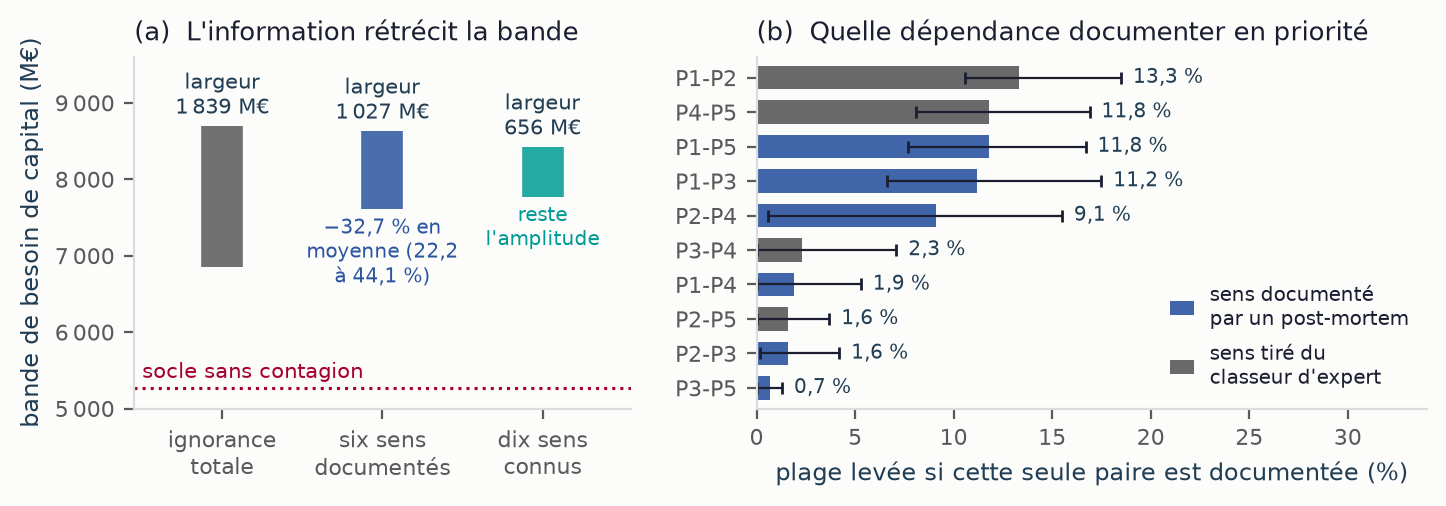
\includegraphics[width=\linewidth]{valeur_information_grille.png}\par\vspace{1mm}
    \footnotesize\textbf{Valeur d'une information $\mathcal I$}
    \[L(\mathcal V)=\sup_{W\in\mathcal V}\mathrm{SCR}(W)-\inf_{W\in\mathcal V}\mathrm{SCR}(W),\qquad
      V(\mathcal I)=1-\frac{L(\mathcal W_{\mathcal I})}{L(\mathcal W)}\in[0,1]\]
    {\scriptsize $\mathcal W$ : matrices admissibles ; $\mathcal W_{\mathcal I}$ : celles compatibles avec $\mathcal I$.\par}
    \column{.31\textwidth}\scriptsize
    {\editorial\color{accent}\large $-32{,}7\,\%$} de plage, sur la grille explorée à $S$ posée, avec les six sens documentés (22 à 44\,\% selon la graine) ;
    {\editorial\color{accent}\large $-57{,}9\,\%$} avec les dix, sans identifier l'amplitude.\par\vspace{2mm}
    {\editorial\normalsize Un registre d'incidents TIC}\par\vspace{1mm}
    Dater la survenance, au mois ou à la semaine.\par
    Classer par domaine de contrôle, pas par vecteur d'attaque.\par
    Consolider une cause commune en un événement à $N$ victimes.\par
    Consigner les piliers qui ont cédé.\par\vspace{2mm}
    Même sans date, la loi des piliers touchés distingue $W$ de $W^\top$ : 62,31\,\% de sinistres multi-piliers sous $W$, 50,77\,\% sous $W^\top$.
  \end{columns}
  \source{rapport, § 10.8, définition de la valeur d'information et figure associée ; quatre graines, grille commune.}
\end{frame}

\begin{frame}{Quel registre d'incidents faudrait-il ?}
  \suivimethode{}{}
  \framesubtitle{\ajout Relier chaque variable du modèle aux champs DORA existants et à l'ajout nécessaire}
  \scriptsize
  \renewcommand{\arraystretch}{1.0}
  \begin{tabularx}{\linewidth}{@{}>{\bfseries\raggedright\arraybackslash}p{.14\linewidth} Y Y Y@{}}
    \toprule
    Variable du modèle & Champ DORA existant & Limite & Ajout nécessaire \\
    \midrule
    Fréquence d'entrée, détection & Dates 2.2, 2.3, 3.2 ; mode de découverte 2.7 & Une horloge par incident, incidents majeurs seuls & Date de défaillance par domaine \\
    \rowcolor{clair}Piliers touchés (loi jointe) & Zones fonctionnelles 3.27 ; causes détaillées 4.2 et 4.3 & Zones et causes ne sont pas les domaines de contrôle défaillants & Domaines P1 à P5, plusieurs valeurs, domaine de première défaillance \\
    Direction de la contagion & Séquence d'événements 4.5 ; mesures temporaires 3.34 & Texte libre, sans ordre codé & Ordre des domaines ayant cédé, sur au moins deux étapes \\
    \rowcolor{clair}Cause commune, accumulation (P4) & Origine tierce, nom et code du prestataire 2.8 ; code de l'autorité 3.1 & Code propre à chaque entité ; tiers renseigné seulement s'il est l'origine & Identifiant d'événement commun, attribué par l'autorité ou le prestataire \\
    Sévérité & Coûts et pertes bruts 4.13 ; recouvrements 4.14 & Un montant par incident, non réparti entre piliers & Répartition par domaine, ou total déclaré indivisible \\
    \bottomrule
  \end{tabularx}
  \vspace{1.5mm}
  \begin{columns}[T,onlytextwidth]
    \column{.48\textwidth}\footnotesize
    \textbf{Trois règles de qualification} (relectures de praticiens) : domaine de première défaillance puis liste des domaines touchés ; identifiant d'événement commun attribué par l'autorité ou le prestataire ; événement déclencheur et mesures de confinement consignés séparément, pour trancher entre un arc de $W$ et un effet sur la détection.
    \column{.48\textwidth}\footnotesize
    Même sans horodatage, la loi jointe des piliers touchés distingue une matrice de sa transposée : $62{,}31\,\%$ de sinistres multi-piliers sous $W$, $50{,}77\,\%$ sous $W^\top$. Ces notifications ne sont pas publiques : nous n'y avons pas eu accès.
  \end{columns}
  \source{rapport, chapitre 10 (§ 10.10 et 10.11). Règlement d'exécution (UE) 2025/302, annexe II ; règlement d'exécution (UE) 2024/2956.}
\end{frame}

\begin{frame}{Comment gouverner le modèle ?}
  \suivimethode{}{}
  \framesubtitle{\ajout Traçabilité, gel de la calibration, validation indépendante}
  \begin{columns}[T,onlytextwidth]
    \column{.31\textwidth}\footnotesize
    {\editorial\normalsize Traçabilité des nombres}\par\vspace{1.5mm}
    Les données étant sous licence, le lecteur dispose des sorties agrégées versionnées. Un programme recherche les nombres de chaque section dans les sorties des scripts cités ; citations externes et valeurs posées sont déclarées avec leur motif, et tout nombre hors contrôle non déclaré est un défaut.\par\vspace{1.5mm}
    {\color{accent}Il confirme l'origine d'un nombre, non son interprétation :} la relecture a trouvé des erreurs de sens parmi les nombres confirmés. Les superlatifs et comptages sont donc calculés dans les scripts.
    \column{.31\textwidth}\footnotesize
    {\editorial\normalsize Gel et registre des limites}\par\vspace{1.5mm}
    Le gel distingue correction d'erreur et changement d'entrée. Les erreurs sont corrigées ; le prix des entrées conservées est déclaré : $+2{,}1\,\%$ sur la fréquence et au moins $+16{,}9\,\%$ sur le quantile de sévérité pour la dérive d'échelle.\par\vspace{1.5mm}
    L'écart de fréquence est recalculé à chaque exécution. Les expériences nouvelles conservent une référence historique et font varier explicitement leurs hypothèses.
    \column{.31\textwidth}\footnotesize
    {\editorial\normalsize Validation indépendante}\par\vspace{1.5mm}
    L'article 124 de la directive Solvabilité II impose la validation d'un modèle interne. Le modèle n'est pas destiné à l'approbation d'un régulateur, mais l'exercice dit ce qui manque. Trois points à examiner :\par\vspace{1mm}
    \textbf{1.} l'additivité des coûts d'un sinistre multi-piliers ;\par
    \textbf{2.} la correspondance état $\to g$, posée et non calibrée ;\par
    \textbf{3.} la stabilité de l'échelle de sévérité, qui dérive.\par\vspace{1.5mm}
    Aucun tiers n'a revu le code ni les calculs : cette validation reste nécessaire avant tout pilotage par le modèle.
  \end{columns}
  \source{rapport, chapitre 10 (§ 10.12). Trois relectures de praticiens, qualitatives, en annexe D.}
\end{frame}

\begin{frame}{Qu'est-ce que ce stage m'a apporté ?}
  \suivimethode{}{}
  \framesubtitle{Un encadrement exigeant, en entreprise et à l'école}
  \begin{columns}[T]
    \column{.47\textwidth}
    {\editorial\normalsize L'apport de l'encadrement}\par\vspace{3mm}
    \small\textbf{Hugo Rapior · Nexialog Consulting}\par\vspace{1mm}
    Un suivi hebdomadaire et disponible, qui a donné au travail sa rigueur et son ancrage métier.
    Il m'a confié la co-écriture de l'analyse actuarielle de l'étude LUCY 2026, publiée par le cabinet.\par\vspace{3mm}
    \textbf{Caroline Hillairet · ENSAE Paris}\par\vspace{1mm}
    Ses travaux sur les états de conformité et l'excitation des sinistres cyber ont nourri le modèle.
    Ses questions ont fait naître deux briques : le quantile prédictif et la sensibilité aux probabilités de propagation.
    \column{.45\textwidth}
    {\editorial\normalsize Ce que je retiens}\par\vspace{3mm}
    \small Vérifier chaque résultat contre le code qui le produit, du premier calcul au dernier chiffre.\par\vspace{3mm}
    Tracer la calibration et chaque correction, pour qu'un tiers puisse tout refaire.\par\vspace{3mm}
    Séparer ce qui est estimé, supposé et non identifié : c'est ce qui rend un capital défendable.
  \end{columns}
  \source{rapport, chapitre « Enseignements du stage ».}
\end{frame}

\begin{frame}{Que permet de défendre ce travail ?}
  \suivimethode{}{}
  {\small\color{ardoise}\bfseries Réponse : dans le scénario, la non-conformité multiplie le besoin de capital par 3,34 ;
  la direction de la contagion, non identifiée, est encadrée par une plage explorée aux sommets.\par}
  \vspace{3mm}
  \begin{columns}[T]
    \column{.30\textwidth}
    \chiffre{$\times\,3{,}34$}{Capital entre deux états de conformité supposés}
    \vspace{1.5mm}\footnotesize L'effet est conditionnel aux quatre canaux et à l'addition des pertes entre piliers.
    \column{.30\textwidth}
    \chiffre{1\,839 M€}{Largeur de la plage explorée aux sommets}
    \vspace{1.5mm}\footnotesize Le sens des liens reste non identifié ; la force des liens est posée.
    \column{.30\textwidth}
    \chiffre{32,7\,\%}{Plage levée en moyenne si six sens sont connus, sur la grille explorée à $S$ posée}
    \vspace{1.5mm}\footnotesize La suite utile est un registre qui renseigne l'ordre et les domaines touchés.
  \end{columns}
  \vspace{2mm}
  {\color{filet}\rule{\linewidth}{.35pt}}\par\vspace{2mm}
  {\editorial\normalsize Ce que la méthode apporte}\par\vspace{2mm}
  \begin{columns}[T]
    \column{.30\textwidth}\footnotesize
    \textbf{1 · Relier conformité et capital}\par
    L'état de chaque pilier déplace quatre canaux de la loi de perte, au lieu d'une pénalité forfaitaire.
    \column{.30\textwidth}\footnotesize
    \textbf{2 · Borner ce qui n'est pas identifié}\par
    $W=S+A$ : $S$ est posée, $A$ parcourt les 1\,024 sommets ; on publie une plage, pas un point.
    \column{.30\textwidth}\footnotesize
    \textbf{3 · Dire quelle donnée collecter}\par
    La valeur d'une information se mesure au rétrécissement de la plage de capital qu'elle produit.
  \end{columns}
  \source{rapport, chapitres 8 à 10 et conclusion. Résultats conditionnels, niveau absolu illustratif ; extrema globaux non démontrés ; élicitation préparée et diffusée, restée sans réponse.}
\end{frame}

{\setbeamertemplate{headline}{}\setbeamertemplate{footline}{}
\begin{frame}[plain]
  \suivimethode{}{}
  \vspace{16mm}\hspace{3mm}{\scriptsize\color{gris}CONFORMITÉ DORA / BESOIN DE CAPITAL}\par
  \vspace{10mm}\hspace{3mm}{\editorial\fontsize{34}{38}\selectfont Merci.}\par
  \vspace{5mm}\hspace{3mm}{\large\color{accent}Place aux questions.}\par
  \vfill\hspace{3mm}{\small Kélian Kaddouri\quad\color{gris}ENSAE Paris · Nexialog Consulting}\par\vspace{8mm}
\end{frame}}

\appendix


% =============================================================================
\section{Annexes}
\begin{frame}{Annexe · Ce qui est calibré, ce qui est posé}
  \suivimethode{}{}
  \framesubtitle{Nature et sensibilité des paramètres (annexe E du rapport)}
  \scriptsize
  \renewcommand{\arraystretch}{1.0}
  \begin{tabularx}{\linewidth}{@{}>{\raggedright\arraybackslash}p{.17\linewidth} >{\raggedright\arraybackslash}p{.17\linewidth} >{\raggedright\arraybackslash}p{.11\linewidth} Y@{}}
    \toprule
    Paramètre & Valeur & Nature & Sensibilité du capital \\
    \midrule
    Indice de queue $\xi$ & 0,5954 (OpRisk) ; PRC 1,03 ; 0,90 en pire cas & calibré, incertain & Forte : de 0,60 à 0,38 quand le seuil monte, dans l'IC90 $[0{,}30\,;0{,}83]$ \\
    \rowcolor{clair}$\sigma$, $u$, $p_u$ & 57,97 M€ ; 20,03 M€ ; 0,15 & calibré & Modérée, via la queue ; $p_u=86/570$ \\
    Fréquence $\lambda$ & $\sim21{,}6$/an (OpRisk) & convention de calage & Sous-linéaire sur le niveau ; 582 événements sur 27 ans \\
    \rowcolor{clair}Multiplicateur de fréquence & $\times1{,}525$ partiel ; $\times2{,}487$ NC & semi-ancré & Forte : canal dominant du chiffre de tête ; $\lambda$ de 41,7 à 65,6 aux bornes \\
    Surdispersion $\varphi$ & 9,20 & posé (prudent) & Élasticité $-0{,}44$ sur l'écart entre états ; 2,24 mesuré \\
    Structure $W=gT/s_{\max}$ & classeur qualitatif & posé / normatif & La direction départage les deux piliers de tête ; surcoût porté par la partie symétrique \\
    \rowcolor{clair}Gain de propagation $g$ & 0,90 ; par état 0,45 / 0,68 / 0,90 & posé & Levier : $\times1{,}6$ sur $[0{,}05\,;0{,}90]$ \\
    Charge systémique $\gamma$ & 0,68 & semi-ancré & Modérée ; proxy de concentration cloud (AWS, Azure, GCP) \\
    \rowcolor{clair}Probabilités d'état NC / PC / C & 0,35 / 0,35 / 0,30 & semi-ancré & Déplace le mélange, pas les états ; enquêtes de conformité (environ 50\,\% non conformes) \\
    Élasticité sévérité/taille $b$ & 0,087 $[0{,}026\,;0{,}148]$ & calibré, tronqué & Faible : $\times0{,}86$ sur la sévérité transposée \\
    \bottomrule
  \end{tabularx}
  \vspace{1mm}
  \source{rapport, annexe E (§ E.1). Trois natures : calibré sur données, posé par jugement d'expert ou choix normatif, semi-ancré sur un proxy externe.}
\end{frame}

\begin{frame}{Annexe · Démonstrations de la cascade}
  \suivimethode{}{}
  \framesubtitle{Loi exacte de l'ensemble atteint, monotonie, co-occurrence, efficience de Shapley}
  \begin{columns}[T,onlytextwidth]
    \column{.49\textwidth}\scriptsize
    \setlength{\abovedisplayskip}{.5mm}\setlength{\belowdisplayskip}{.5mm}
    \textbf{Loi exacte (proposition 5.4).} $\{S_a=A\}$ est l'intersection de deux événements portant sur des arêtes disjointes, donc indépendants : aucune arête ne sort de $A$ (probabilité $B(A)=\prod_{j\in A,k\notin A}(1-W_{jk})$) et $a$ atteint tout $A$ par les arêtes internes (probabilité $R(A)$).
    \[R(A)=1-\sum_{\substack{A'\subsetneq A\\ a\in A'}}R(A')\prod_{j\in A',\,k\in A\setminus A'}(1-W_{jk}),\qquad R(\{a\})=1\]
    \textbf{Monotonie stochastique (proposition 5.5).} Couplage par des uniformes $(U_{jk})$ communes : l'arête $j\to k$ est vivante si $U_{jk}<M_{jk}$. Si $W\le W'$ terme à terme, le graphe sous $W$ est un sous-graphe de celui sous $W'$, et l'accessibilité croît par ajout d'arêtes : $S_a(W)\subseteq S_a(W')$ presque sûrement. En revanche, une perturbation antisymétrique élève $W_{jk}$ en abaissant $W_{kj}$ : aucune monotonie coordonnée ne garantit l'optimum aux sommets du pavé.
    \column{.47\textwidth}\scriptsize
    \textbf{Co-occurrence (proposition 5.7).} Pour atteindre $j$ et $k$ depuis une amorce $a\notin\{j,k\}$, il faut au moins deux arêtes vivantes, d'où un terme en $O(\|W\|^2)$ ; depuis $j$, le pilier $k$ est atteint avec probabilité $W_{jk}$, et inversement. Le terme d'ordre un, $2rS_{jk}$, est le même pour $W$ et $W^\top$.\par\vspace{1mm}
    \textbf{Contre-exemple d'ordre deux.} Trois piliers, $W_{12}=W_{13}=w>0$, autres entrées nulles. Sous $W$, une amorce en 1 touche 2 et 3 ensemble avec probabilité $w^2$ ; sous $W^\top$, aucun sinistre ne touche 2 et 3 ensemble. Même partie symétrique : la co-occurrence d'ordre deux distingue la fourche du collisionneur (structure en V de l'identification des graphes causaux).\par\vspace{1mm}
    \textbf{Efficience de Shapley.} $\varphi_i=\frac1{n!}\sum_\pi\big[v(P_i(\pi)\cup\{i\})-v(P_i(\pi))\big]$ ; à permutation fixée la somme des contributions marginales est télescopique et vaut $v(\{1,\dots,n\})$. L'attribution est une \emph{partition} du surcoût, non une prédiction du retrait d'un pilier.
  \end{columns}
  \source{rapport, annexe A. Avec cinq piliers, les $5!$ permutations et les 25 valeurs de $v$ sont énumérées en entier : pas d'erreur d'approximation combinatoire.}
\end{frame}

\begin{frame}{Annexe · Une queue par pilier, le pilier des tiers}
  \suivimethode{}{}
  \framesubtitle{Adaptations par pilier (annexe C du rapport)}
  \begin{columns}[T,onlytextwidth]
    \column{.49\textwidth}\scriptsize
    {\editorial\normalsize Queue de sévérité par pilier}\par\vspace{1mm}
    Une seule queue $\xi$ est appliquée aux cinq piliers. La queue est pourtant hétérogène selon la catégorie bâloise : $\xi$ varie de $0{,}87$ (Employment) à $1{,}37$ (Execution, Delivery \& Process Management), dispersion $0{,}50$. L'assignation aux piliers n'est pas un fait : la catégorie la plus proche des TIC compte 111 observations, sous le seuil d'estimation de 150.\par\vspace{1mm}
    Nous énumérons les 120 assignations des cinq queues observées aux piliers. À moyenne des queues fixe, donner à chaque pilier sa propre queue relève le capital de $+55\,\%$ à $+96\,\%$ : la VaR croît plus vite que linéairement en $\xi$, \textbf{une queue commune sous-estime donc le capital}. Le pilier de tête reste dominant dans $83\,\%$ des 30 assignations tirées.\par\vspace{2mm}
    {\editorial\normalsize Accumulation chez un prestataire}\par\vspace{1mm}
    P4 n'est pas un nœud de cascade comme les autres : un prestataire partagé dégrade plusieurs piliers à la fois (MOVEit : 191 victimes d'un seul choc). Nous lui substituons un choc commun de probabilité $\omega$ ; c'est une co-occurrence symétrique, la seule structure entre piliers que la donnée soutienne.
    \column{.47\textwidth}\scriptsize
    L'intensité $\omega$ n'est pas identifiée au sein d'une entité isolée : nous la bornons sur $[0,\gamma]$, $\gamma=0{,}68$. À $\omega=\gamma$, la dépendance partagée emporte en moyenne $3{,}7$ piliers d'un coup, soit $+19\,\%$ de capital par rapport au traitement en nœud de cascade. La probabilité qu'un incident P4 touche au moins trois piliers passe de $0{,}22$ à $0{,}90$.\par\vspace{1.5mm}
    \renewcommand{\arraystretch}{1.12}
    \begin{tabularx}{\linewidth}{@{}Y r r@{}}
      \toprule
      Co-déclenchement de P4 & Gaussienne & Gumbel ($\theta=1{,}8$) \\
      \midrule
      Dépendance de queue $\lambda_U$ & 0 & 0,53 \\
      Cinq piliers avec P4 & 0,17 & 0,39 (facteur 2,3) \\
      \bottomrule
    \end{tabularx}\par\vspace{1.5mm}
    Nous ne tranchons pas la copule : le co-déclenchement se lit en bande, à $\tau$ de Kendall égal. La fréquence marginale d'un pilier reste $p_4=0{,}15$ dans les deux cas. Le co-déclenchement d'un autre pilier tient dans $[0{,}48\,;0{,}58]$, sous la borne $\gamma$, qui reçoit ainsi une origine structurelle.
  \end{columns}
  \source{rapport, annexe C (§ C.1 et C.2). La vue inter-clients (centaines d'entités victimes de MOVEit) sort du capital par entité.}
\end{frame}

\begin{frame}{Annexe · Détection, tiers et temps d'arrêt}
  \suivimethode{}{}
  \framesubtitle{Détection comme courbe de survie, ancrages européens, déclenchement de P4}
  \begin{columns}[T,onlytextwidth]
    \column{.33\textwidth}\scriptsize
    {\editorial\normalsize Détection de P2 et P3}\par\vspace{1mm}
    Le délai de découverte en finance (VCDB, $n=278$) est bimodal : $47\,\%$ des incidents sont découverts le jour même, $8\,\%$ en semaines, $45\,\%$ en mois ou plus. La matérialité vient des découvertes lentes : $\pi_{\mathrm{slow}}=0{,}45$.\par\vspace{1mm}
    L'élasticité de la détection à la maturité n'est pas mesurée : le surcoût du seul canal est une bande, de 1\,775 à 8\,052 M€. Le multiplicateur $0{,}85\,/\,1{,}20$ est retrouvé pour $\eta\approx0{,}36$ : un point de la courbe, non un choix arbitraire.
    \column{.31\textwidth}\scriptsize
    {\editorial\normalsize Ancrages européens}\par\vspace{1mm}
    Le premier rapport DORA des autorités européennes établit que $29\,\%$ des 3\,383 incidents TIC majeurs de 2025 proviennent d'un tiers : P4 est une amorce majeure, ce que le classeur posait par jugement (ROOT$_4=0{,}90$).\par\vspace{1mm}
    L'analyse des registres d'externalisation par la BCE : plus de $30\,\%$ du budget des grandes banques va à 10 fournisseurs, $50\,\%$ du budget critique à 30 ; 19 fournisseurs TIC critiques désignés. Ces chiffres ancrent $\gamma=0{,}68$ sur une mesure de concentration officielle.\par\vspace{1mm}
    La taxonomie fine du tiers est trop rare dans la donnée ouverte : 20 incidents en finance dans OpRisk.
    \column{.31\textwidth}\scriptsize
    {\editorial\normalsize Déclenchement de P4}\par\vspace{1mm}
    Si le facteur tiers est un brownien standard, le déclenchement est un temps de premier passage :
    \[\mathbb P(\tau\le T)=2\,\Phi\Big(\frac{-z^\star}{\sqrt T}\Big)=2\,\mathbb P(Z_T\ge z^\star)\]
    (principe de réflexion : propriété de Markov forte et symétrie des accroissements). La lecture dynamique vaut le double de la statique.\par\vspace{1mm}
    À $\rho=0{,}50$ : $0{,}14$ en moins d'un an, délai médian d'environ cinq ans ; à $\rho=0{,}75$ : $0{,}23$, médian d'environ trois ans.\par\vspace{1mm}
    Le délai d'un brownien pur est d'espérance infinie ; un facteur à retour à la moyenne serait plus réaliste. Aucun test de martingalité n'est conduit ; $z^\star$ vient de la calibration.
  \end{columns}
  \source{rapport, annexe C (§ C.2.2, C.2.3 et C.3). Autorités européennes de surveillance (2026) ; Banque centrale européenne (2024).}
\end{frame}

\begin{frame}{Annexe · Questions que le jury peut poser}
  \suivimethode{}{}
  \framesubtitle{Réponses courtes, avec leur appui dans le rapport}
  \scriptsize
  \renewcommand{\arraystretch}{1.12}
  \begin{tabularx}{\linewidth}{@{}>{\bfseries\raggedright\arraybackslash}p{.27\linewidth} Y p{.09\linewidth}@{}}
    \toprule
    Question & Réponse & Appui \\
    \midrule
    Le facteur 3,34 est-il un effet de DORA mesuré ? & Non : il compare deux états de conformité posés ; aucune entité ne publie son état. Le signe de l'écart tient sur toutes les correspondances testées ; l'amplitude est un scénario. & § 9.1, 6.4 \\
    \rowcolor{clair}Pourquoi $b_\lambda=\sqrt{0{,}074}$ en lecture centrale ? & C'est le milieu géométrique du registre ($0{,}074$) et de la proportionnalité ($1$), posé faute de donnée qui sépare les deux. On juge l'ordre qu'il produit : le grand groupe vaut 19,5 fois l'assureur B, contre 2,9 en lecture du registre. & § 9.10, 9.11 \\
    Peut-on backtester le quantile à 99,5\,\% ? & Non : détecter un taux de dépassement doublé demanderait 1\,811 années. Le backtest valide le centre et le corps, et déclare une dérive d'échelle. & § 4.7 \\
    \rowcolor{clair}Que change l'inversion de la direction ? & Retourner $W$ déplace le capital de $3{,}6\,\%$ (295 M€) et la priorité de P1 à P4 ; sur l'ensemble admissible, l'écart atteint 1\,173 M€. D'où des bornes, non un point. & § 5.9, 8.2 \\
    Pourquoi une cascade plutôt qu'un Hawkes ? & Une cascade sans auto-excitation donne un ratio de branchement de $0{,}480$ contre $0{,}551$ mesuré : le Hawkes n'est pas distinguable. Par parcimonie, la cascade décrit aussi la structure entre piliers. & § 10.3 \\
    \rowcolor{clair}Pourquoi additionner les coûts des piliers touchés ? & C'est l'hypothèse structurelle la plus lourde, non testée. Un exposant $\theta\in[0{,}70\,;1{,}30]$ déplace l'écart de 9\,706 à 20\,487 M€ ; signe et ordre tiennent, pas l'amplitude. & § 10.8 \\
    Pourquoi le besoin est-il nul pour une petite entité ? & La probabilité annuelle d'une charge de queue positive est sous $0{,}5\,\%$ ; les incidents comptés ne sont pas tous des pertes positives. Bascule centrale : 2\,517 M€, sans domaine de validité démontré. & § 9.11 \\
    \bottomrule
  \end{tabularx}
  \source{rapport, chapitres 4, 5, 8, 9 et 10.}
\end{frame}


\end{document}
